%% LyX 2.1.4 created this file.  For more info, see http://www.lyx.org/.
%% Do not edit unless you really know what you are doing.
% Original obtained on 02/25/19 from : https://github.com/drwillis/uncc-thesis-latex
\documentclass{UNCC-thesis}
\usepackage[T1]{fontenc}
\usepackage[latin9, utf8]{inputenc}
\setcounter{secnumdepth}{3}
\usepackage{array}
\usepackage{float}
\usepackage{graphicx}
\usepackage{nomencl}
\usepackage{xcolor}
\usepackage{csvsimple}
\usepackage{hyperref}
\hypersetup{
    colorlinks=true,
    linkcolor=black,
    filecolor=black,      
    urlcolor=cyan,
    citecolor=black,
}
\usepackage{longtable}
% the following is useful when we have the old nomencl.sty package
\providecommand{\printnomenclature}{\printglossary}
\providecommand{\makenomenclature}{\makeglossary}
\makenomenclature

\makeatletter

%%%%%%%%%%%%%%%%%%%%%%%%%%%%%% LyX specific LaTeX commands.
%% Because html converters don't know tabularnewline
\providecommand{\tabularnewline}{\\}

%%%%%%%%%%%%%%%%%%%%%%%%%%%%%% User specified LaTeX commands.
% If you are using MikTeX on Windows and you have a nomenclature section
% you may want to uncomment the line below.
%
%\immediate\write18{makeindex phdthesis.nlo -s nomencl.ist -o phdthesis.nls}

\@ifundefined{showcaptionsetup}{}{%
 \PassOptionsToPackage{caption=false}{subfig}}
\usepackage{subfig}
\makeatother
\usepackage{rotating}

\begin{document}
\pagenumbering{roman}
\fbmatterchapterformat
% Doctype should be either dissertation proposal, dissertation, or thesis.
% If you're getting a master's, specify "thesis" below.  
% If you're getting a PhD, specify "dissertation" below.
\doctype{dissertation}
%%%%%%%%%%%%%%%%     IMPORTANT! IMPORTANT! IMPORTANT! %%%%%%%%%%%%%%%%
% The rules below MUST be followed for the abstract page and chapter titles
% to be correctly formatted.
%
% 1. Only the first letter of the entire title should be capitalized to allow the 
%    title to appear as required by the graduate school on the Abstract page.
% 2. Write chapter titles in ALL CAPS.
%
\title{ Nutritive Knowledge Based Discovery: Enhancing Precision Nutrition Hypothesis Generation. }
\author{Aaron Trautman}
\degree{Doctor of Philosophy}
\major{Bioinformatics and Computational Biology}
\publicationyear{2022}

\advisor{Dr. Cory Brouwer}

% Add the full name and title of all your committee members,
% apart from your advisor, one by one.  The style file expects
% 3 to 5 committee members in addition to your advisor.

\committeeMember{Dr. Robert Reid}
\committeeMember{Dr. Cynthia Gibas}
\committeeMember{Dr. Way Sung}
\committeeMember{Dr. Xiaoxia Newton}

% Generate the preliminary title page and copyright page.
\maketitlepage
\makecopyright
\begin{abstract}
Diet-related diseases like obesity and type-2 diabetes are on the rise. Precision nutrition, a way to tailor dietary requirements for each individual, is heralded as a solution to these problems. However, nutritional research is held within sparse, siloed resources that rarely connect, which leads to significant barriers hindering the progress of precision nutrition. Three knowledgebases were produced as a result of this work. The ABCkb 1.0 overcomes these barriers by linking 11 separate resources in the path from plants to disease through molecular mechanisms. This resource is built in Neo4j and provides a web-based interface available for browsing (https://abckb.charlotte.edu). A second knowledgebase, ABCkb 2.0 connects microbiota information to diet and human health through the incorporation of text-mined associations from full text articles. The final knowledgebase produced links long-covid to dietary components through possible molecular mechanisms. These three knowledgebases promote progress in precision nutrition to tackle the rise in diet-related disease.

\end{abstract}
\begin{dedication}
%If you decide to have a dedication page, your dedication text would
%go here.
%
%The Dedication page, if used, pays a special tribute to a person(s)
%who has given extraordinary encouragement or support to one's academic
%career.
To my wife. Thank you is not enough for all of the support you have given to me over the years.

\end{dedication}
\begin{acknowledgements}

A huge thank you to all who have supported this work and my educational journey. I fully appreciate my advisor whose guidance was invaluable to completing this work. I appreciate the librarians from UNC Charlotte for securing rights to text-mine full text articles and the patience they demonstrated. The Plant Pathways Elucidation Project provided graduate funding along with interns who supported the knowledgebase work. A huge thank you to Steven Blanchard for all the IT support provided and guidance writing better code. Of course this work would not be possible without the help of all my fellow classmates and co-laborers but specifically: Richard Linchangco, and Aneeta Uppal. Thank you to all of the P2EP interns who worked on this project: Logan Kavanaugh, Chris Williams, Aswani Unnikrishnan, Kiera Patanella, Natalie Kratts, Kevin Selles, and Daniel Firo. 

\end{acknowledgements}
%If you decide to have a acknowledgements page, your acknowledgement
%text would go here.
%
%The Acknowledgement page should be brief, simple, and free of sentimentality
%or trivia. It is customary to recognize the role of the advisor, the
%other members of the advisory committee, and only those organizations
%or individuals who actually aided in the project. Further, you should
%acknowledge any outside source of financial assistance, such as GASP
%grants, contracts, or fellowships.
%\end{acknowledgements}
\tableofcontents{}

\listoftables{}


\listoffigures{}


\newpage
\renewcommand{\nomname}{LIST OF ABBREVIATIONS}
% uncomment line below to title your nomenclature list as LIST OF SYMBOLS
%\renewcommand{\nomname}{LIST OF SYMBOLS}
%
% NOTE: IF YOU USE A LIST OF ABBREVIATIONS / LIST OF SYMBOLS and are using command-line LaTeX (not LyX) 
% YOU MUST COMPILE THE NOMENCLATURE INDEX
% example:
% bash$> pdflatex msthesis.tex
% bash$> makeindex msthesis.nlo -s nomencl.ist -o msthesis.nls
% bash$> pdflatex msthesis.tex
%
\addcontentsline{toc}{chapter}{\nomname}\settowidth{\nomlabelwidth}{ECE}
\printnomenclature{}

\nomenclature{KB}{KnowledgeBase}
\nomenclature{IBS}{Irritable Bowel Syndrome}
\nomenclature{IBD}{Inflammatory Bowel Disease}
\nomenclature{NLP}{Natural Language Processing}
\nomenclature{WGS}{Whole Genome Sequencing}
\nomenclature{HetERel}{Heterogeneous Edge-adjusted Relevance}
\nomenclature{WMS}{Whole Metagenomic Sequencing}
\nomenclature{NCBI}{National Center for Biotechnology Information}
\nomenclature{T2D}{Type 2 Diabetes}

\newpage
\setcounter{page}{1}
\pagenumbering{arabic}
% 2 inch top spacing for new chapters
\bodychapterformat
%\begin{preface}
%\end{preface}

% Introduction outline

% Summary of the problem (Capture the reader's interest)
%   - Diet-related diseases rising
%   - Gut microbiome diseases, rising
%   - Biological research spread out in many places makes it        hard for research to continue
% Previous Knowledgebase work (or previous work on nutri dbs)
    % - Richard's work (primarily theoretical)
    % - Problems
    %     - Hard to use
    %     - Out of date
    %     - Required a lot of computational resources
    %     - Never really implemented
    %     - Never published
    %     - Lots of unnecessary data
    % - Graphs for full (maximum) effect

% Microbiome Research 
    % - History
    % - Where we are now
    % - Current problems still left to solve
    % - Highlight disparate sources

% Public collections of data
    % Ontologies
    %     - Strengths
    %     - Weaknesses
    %     - Common Examples
    % Databases
    % - Relational Database Management Systems
    %     - Strengths
    %     - Weaknesses
    %     - Common examples
    % - GDBMS
    %     - Strengths
    %     - Weaknesses
    %     - Common Examples
    % - Structured vocabularies

% NLP associations
    % - NLP is hard
    %     - Entity extraction
    %     - Sentence parsing
    %     - Tasks
    %     - Different methods
    %     - Some different tools
    %         - Few developed for scientific literature
    %         - Open source
    %         - Enterprise, enter I2E

\chapter{INTRODUCTION}

Diet-related, noncommunicable diseases are rising in developing countries worldwide. One of these diseases, Irritable Bowel Syndrome (IBS) a functional disorder defined primarily by its symptoms, affects around 11\% of the world's population with prevalence in America reaching as high as 20\%\cite{canavan_epidemiology_2014}. Other diet-related noncommunicable diseases including heart disease, type 2 diabetes (T2D), various respiratory diseases, and some cancers contribute to 71\% of all deaths worldwide\cite{world_health_organization_non_2021}. Several studies have revealed nutritive connections to these diseases which has driven many public-policy decisions in an attempt to combat this rise\cite{greenberg_diet_nodate,olatona_dietary_2018, hunter-adams_health_2020}. However, many of these studies have not established the molecular mechanisms contributing to these nutritive connections. Further complicating understanding the connections is the interaction of the human gut microbiome with dietary components which produce secondary and tertiary metabolites that impose specific symptoms on host biology\cite{agus_gut_2021,oliphant_macronutrient_2019}. This lack of knowledge hinders the ability to define and characterize optimal human health.  

\section{Knowledge Based Discovery}

Literature-based discovery was first described by Don Swanson after discovering the molecular connections between Raynaud syndrome and fish oil in 1986\cite{smalheiser_rediscovering_2017}. He did this by manually reading a corpus of abstracts on Raynaud syndrome, a disease that affects blood flow to the extremities under extreme temperatures and stress. He discovered the associated effects of Raynaud's on blood viscosity, platelet aggregation, and further read through corpii of abstracts on the associated topics. This lead to the discovery of Fish Oil as a candidate therapeutic for the symptoms of Raynaud syndrome\cite{swanson_fish_2015}. This process, though tedious and time-consuming, is how scientific discovery usually occurs. Scientific discoveries are communicated through unstructured literature, journal articles, and then rediscovered by readers. However, structured resources like databases and queriable ontologies facilitate a more efficient method of discovery.

Significant effort has been put into the development of resources to catalogue and expedite scientific discovery. The National Center for Biotechnology Information (NCBI) currently maintains a total of 39 databases \cite{sayers_database_2021}. The Nucleic Acids Research journal from Oxford Academic hosts a repository of over 1,600 databases with their categories and publishes an annual database report \cite{rigden_2021_2021}.

Often researchers develop databases surrounding an individual topic of study. Interfaces are subsequently developed to browse and query the contents of these databases. To explore the contents, users perform searches and then download the results. Cross-referencing these results with other resources, requires manual connection of these resources. Difficulties arise when researchers attempt to cross-reference separate resources that use unique identifiers specific to each resource. The same resources generated to aid scientific discovery create a significant barrier to produce testable hypotheses. The urgency of increasing and prevalent diet-related diseases combined with limited knowledge of molecular mechanisms in the pathway of plants to human health, along with the significant barrier of a multiplicity of resources create an interesting challenge to solve.


%The NCBI hosts a catalogue of scientific journal articles which researchers can browse using Medical Subject Headings to enhance queries. The NCBI also produces a gene database of gene names, synonyms, and taxonomic data with additional genomic information corresponding to each gene when available.

\section{Nutritional Resources}

Scientific resources are scattered throughout many platforms, and none fully capture the molecular mechanisms by which plants and plant compounds affect human health \cite{trautman_aliment_2021}. NutriChem was developed by text-mining MEDLINE abstracts using a naive bayesian classifier to identify pairs of plants, from NCBI Taxonomy database, and human disease phenotypes \cite{jensen_nutrichem_2015}. More recently, NutriChem 2.0 has focused primarily on drug-plant associations which can provide informative information on how efficacy of specific drugs may be affected by consumption of particular plants \cite{ni_nutrichem_2017}.  One major drawback of the resulting database is the lack of chemical-gene associations, a key component to determine known molecular mechanisms and develop nutritive hypotheses. In addition, the database is no longer available from their web-browser, a key feature of many biological databases (Figure ~\ref{fig_1_1}).

\begin{figure}[!h]
{\begin{centering}
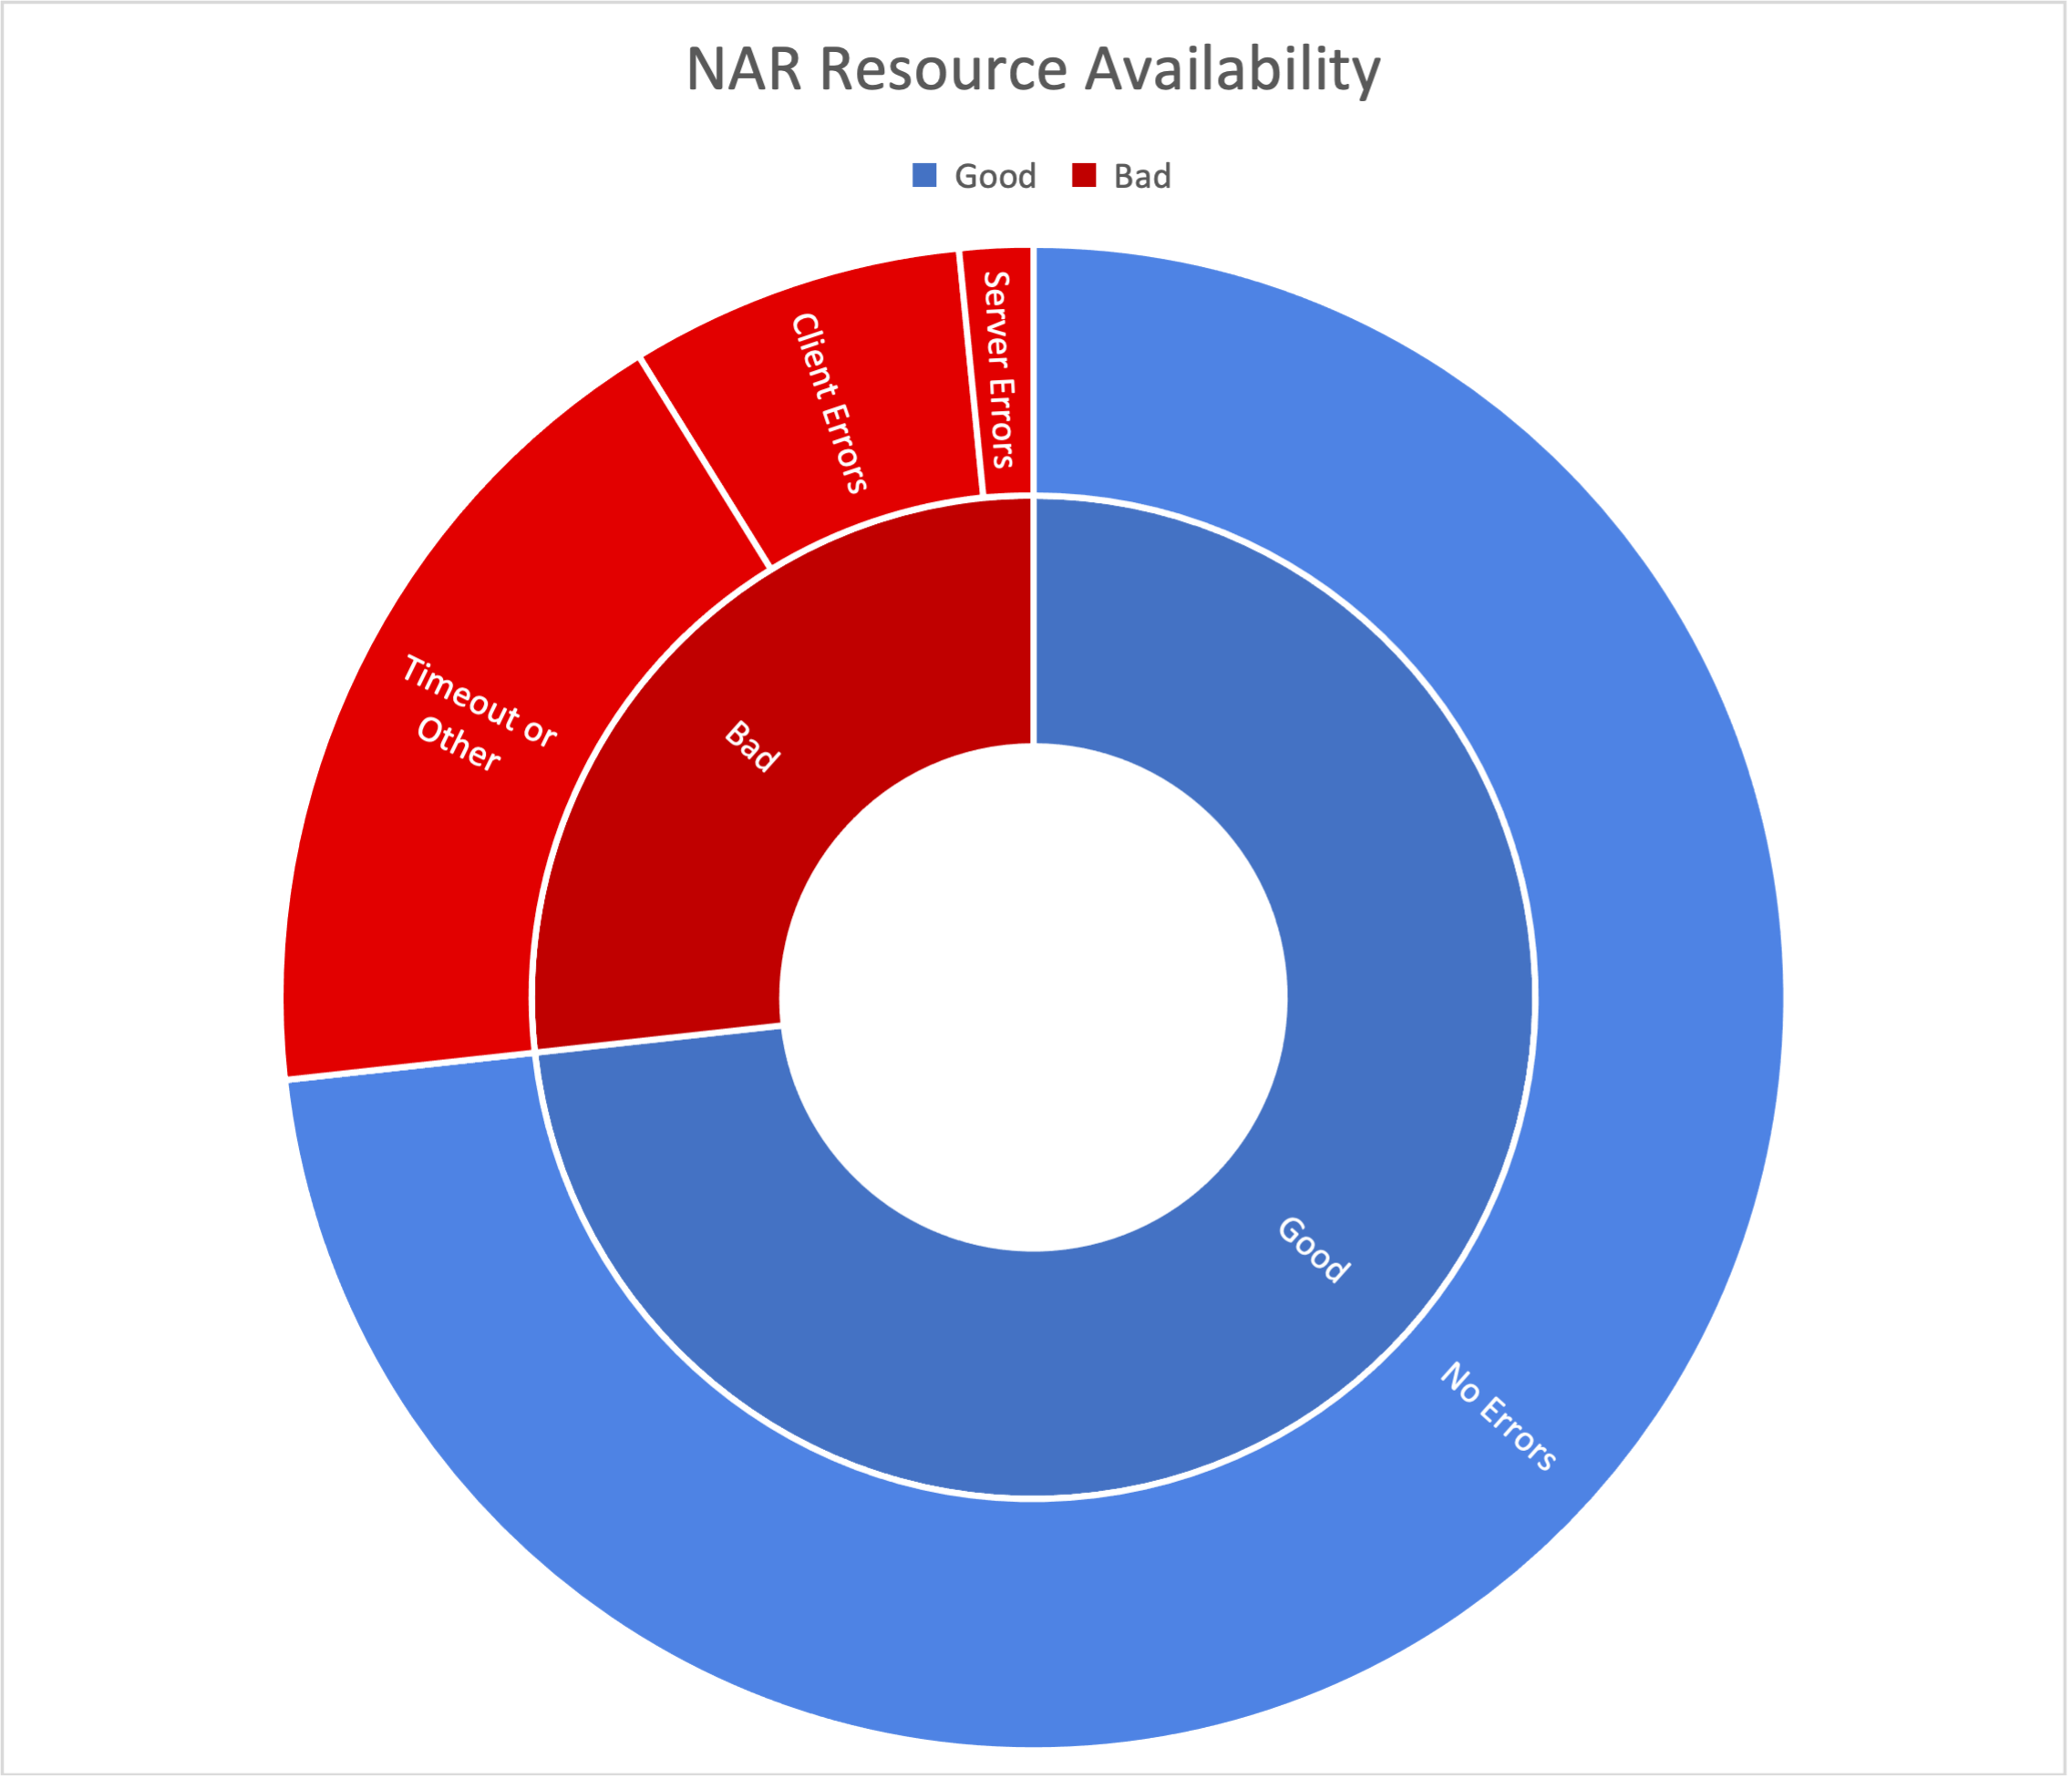
\includegraphics[height=5in]{figs/Fig_1_1.png}
\par\end{centering}}
\caption[NAR Resource Availability]{\label{fig_1_1} Going through all of the available biological resources and databases listed on the NAR, all of the links found on the page were examined for availability and categorized as good, with a url response code of 200 or bad, with response codes grouped by type.}

\end{figure}

One of the more comprehensive resources available is the Comparative Toxicogenomics Database (CTD) \cite{davis_comparative_2019}. The CTD provides users with manually curated associations from chemicals, genes, pathways, and phenotypes. Apart from the time and resources required to develop manually curated connections, the main disadvantage of utilizing this resource for nutritive research is the lack of plant-chemical associations.

Plant-chemical associations can be found in other databases, but are often highly specialized to a specific plant or chemical group. The PhenolExplorer database catalogues plant polyphenol components with quantitative amounts \cite{rothwell_phenol-explorer_2013}. However, PhenolExplorer was last updated in 2016 and only contains phenolic compounds. Other resources exist to categorize flavor components of food without the medical components. As a general resource, FooDB provides many possible chemical components of plants with quantitative information and mappings to external resources \cite{noauthor_foodb_nodate}. This resource is frequently updated, however the quantitative chemical amounts are often less informatively provided as a "trace amount." 

\section{Previous Knowledgebase Research}

Manually connecting data from separate, isolated resources delays research in the information gathering phase. Previous research from Richard Linchangco resulted in a Knowledgebase (KB) which could provide nutrition research a path to develop new evidence-based hypotheses aiding the discovery of molecular mechanisms between dietary plants on human phenotypes through a path of Plant -> Chemical -> Gene -> Pathway -> Phenotype \cite{linchangco_semantics_2018}. The KB was created in Neo4j, a graph database management system and contained nodes with labels: Organisms, Plants, Chemicals, Genes, Pathways, and Phenotypes all extracted from a combination of resources. Connections were extracted from both public resources and associations derived from Natural Language Processing (NLP) of over 30 million abstracts from the MEDLINE index. This KB was not without limitations.

One major drawback of this KB is the technical skill required to utilize it. Neo4j uses Cypher Query Language to retrieve data within the graph database. Users are required to create complex queries to extract data, and connect associations. Additionally, the data contained within was quickly out of date with no way to extract, transform, and load new, up-to-date data. Another issue with the KB design is the large edge density of the graph database which significantly hindered graph traversal and exploration. Edge density is simply the relative amount of edges, or connections, between nodes. Significant effort was spent reducing predicates into more informative edge labels which yielded some node pairs containing upwards of 20 edges. Graph traversal time is dependent on both the amount of nodes, and connections. Thus, queries from Plants to Phenotypes required significant computational resources to complete, and an unreasonable amount of time (Figure ~\ref{old_kb_graph}). 

\begin{figure}[!h]
{\begin{centering}
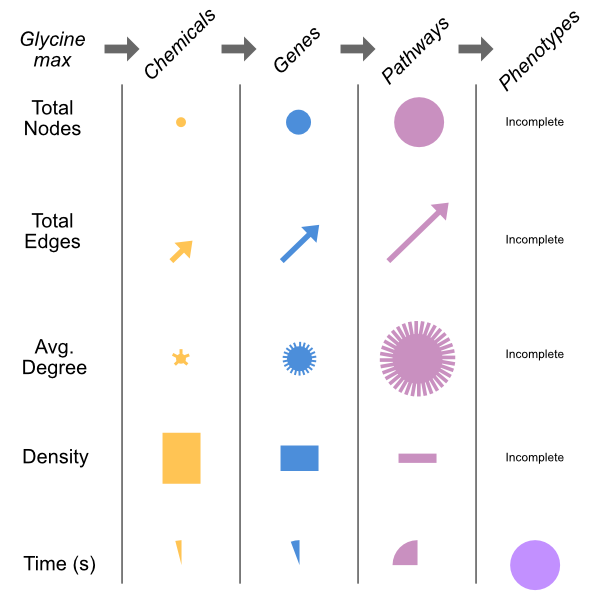
\includegraphics[height=6in]{figs/Old_KB_Stats_Graph.png}
\par\end{centering}}
\caption[Old ABCkb Statistics]{\label{old_kb_graph} A query was run on the old ABCkb from Soybean (\textit{Glycine max}) to Chemicals, Genes, Pathways, and Phenotypes on a 1 TB memory cluster at UNC Charlotte. The time it took to produce the results was logged and the query to phenotypes maxed out after a day, returning no results.}

\end{figure}

The KB was also never published, never fully implemented, and contained data that added little value to the original goal, providing molecular mechanisms from plants to human health. Finally, as microbiome research has progressed, an additional piece of nutritional research missing from the KB is the contribution from gut microbiota on diet and human health.


\section{Microbiome Research}

The gut microbiome is formally defined as the collection of bacterial genomes contained within the gut, while the term microbiota refers to the set of bacterial species ~\cite{ursell_defining_2012}. The two terms are used interchangeably, but it is worth noting the difference. There is a rich history of microbiome research yielding knowledge of a functioning bacterial community existing within healthy organisms\cite{prescott_history_2017,aminov_brief_2010}. \textit{Escherichia coli} was found naturally occurring in the gut of infants in the 1800's\cite{shulman_theodor_2007}. However, it wasn't until the 1960's that the acceptance of a gut microbiome became more widespread\cite{lloyd-price_healthy_2016}. Many microbiota have only recently been discovered due to their inability to grow in culture. This is in part, due to the technological advancements in genome sequencing over the past 20 years. These advancements have lead to cheaper sequencing costs, greater depth and coverage, better assemblers, and the incorporation of microbiome strategies into many biological analyses. Increases in the specificity of assays have also led to taxinomic reclassification of known species like \textit{alistipes} from \textit{bacteroides} \cite{rautio_reclassification_2003}. There are several microbiome pipelines available with strengths and weaknesses alike.

\subsection{Microbiome Pipelines}

Researchers have many options when performing a gut microbiome study, most of which borrow from traditional genomic analyses. 16S sequencing, the most prevalent approach, quantifies a region of the 16S gene from bacterial taxa found in stool samples \cite{johnson_evaluation_2019}. Shotgun Whole Metagenomic Sequencing (WMS) is becoming more common and attempts to reconstruct whole metagenomes from stool samples \cite{sharpton_introduction_2014}. A challenge with WMS is assembling multiple small genomes with many fragments of random sizes. Another pipeline is metatranscriptomics which attempts to characterize all of the expressed genes within a sample \cite{shakya_advances_2019}. This allows detection of active community members, and may provide insights on how diet affects microbiota gene expression.

\subsubsection{16S Sequencing}

16S sequencing targets ribosomal DNA of bacteria in a sample, is cost effective, works with most sample types, and provides taxonomic classification into the family level~\cite{janda_16s_2007}. This is useful for detecting broad shifts in microbiota composition. The 16S gene contains nine hypervariable regions that can be amplified through simple Polymerase Chain Reaction (PCR) methods, however the v4 region is often the target of these analyses ~\cite{pichler_16s_2018}. Primers are generally universally applicable, as the 16S gene is highly conserved which further decreases the costs of microbiome analyses. In addition, Illumina sequencers are frequently chosen for sequencing amplified 16S regions. However, 16S sequencing does not separate bacterial strains well, which is necessary for a more detailed look at microbiota composition ~\cite{noauthor_16s_nodate}.

\subsubsection{Whole Metagenome Sequencing}

To quantify microbiome composition at a species-strain level, Whole Metagenome Sequencing (WMS), also called shotgun sequencing, is used to capture all of the genomic data within a sample~\cite{noauthor_16s_nodate}. This method utilizes any high-throughput sequencer with Illumina or Pac-Bio being the most common. Sequenced WMS reads are mapped to a reference database to remove host contamination and identify strains and species present within the sample~\cite{bharti_current_2021}. Abundances are estimated from mapped reads that align to bacterial reference genomes in a greater resolution than 16S sequencing~\cite{noauthor_16s_nodate}. Limitations of shotgun sequencing include the generation of random DNA sequences that are either too small to align with any confidence, or too low in quality~\cite{bharti_current_2021}. Different versions of WMS attempt to capitalize on the resolution of this method while adding additional strengths. Phase Genomics adds a Hi-C method in conjunction with WMS to tagment DNA sequences which facilitates genome assembly after sequencing~\cite{press_hi-c_2017}. This tagmentation method aids in genome fragment reconstruction by linking sequences that are close in proximity. Though sequencing costs have decreased in recent years, WMS is still an expensive method for a large volume of samples~\cite{noauthor_16s_nodate}.

% \subsubsection{Metatranscriptomics}

% While 16s and whole metagenome sequencing approaches provide a window into the microbiota present within the gut, they do not specifically target expressed microbial genes. Metatranscriptomic approaches target expressed genes to give a functional profile of active microbiota under differing 

%This led to the discovery of gut dysbiosis, a condition where bacterial communities are in disarray, and is connected with many conditions like hypertension, IBS, IBD, diabetes, and obesity\cite{carding_dysbiosis_2015}.

\subsection{Current State} % expand!!!!!

Associations between specific gut microbiota and human phenotypic outcomes have been established from these different methods. Increases in bifidobacteria in the human gut are associated with reductions in colorectal cancer ~\cite{bahmani_anti-colon_2019}. Clear links between \textit{Helicobacter pylori} and stomach ulcers, which often leads to gastric cancer, have also been established~\cite{graham_history_2014}. Given the discovery of gut disbiosis, an increase in pathogenic bacteria, opportunistic bacteria, or decreases in beneficial bacteria, determining optimal gut microbial composition was a goal of the human microbiome project~\cite{turnbaugh_human_2007}. Controversially, no one specific microbiota composition has been identified to provide favorable phenotypic outcomes over another. Increased abundances of beneficial microbiota, called probiotics, have been found to provide benefits to the host which has led to an increasing interest in the discovery of interaction with dietary components~\cite{markowiak_effects_2017}. Strong interacting components driving microbiota variance include diet, host gender, environment, geographical location, and ethnicity~\cite{national_academies_of_sciences_microbiome_2017}. 

Some associations between phytochemicals and these beneficial gut microbiota have been established which has led to the development of prebiotics. These are specific nondigestible nutrients that are selectively fermented to facilitate the growth of probiotic bacteria and can be supplied by diet\cite{bindels_towards_2015}. For example, members of the genus Bifidobacterium commonly supplied in probiotic supplements are benefited by non-digestible oligosaccharides that can be found in oats\cite{grootaert_microbial_2007}. Both Avena sativa and Bifidobacteria have been linked to a reduction in colon cancer\cite{bindels_towards_2015,prado_ingestion_2019}. This raises interesting questions for nutrition researchers. Are the phytochemical associations produced from in vitro experiments fully representing the health benefits of plants? How does the microbiome contribute to human health and what are the associations from the foods we eat to the bacteria in our gut, and how does this all correspond to human health? Experimental designs that exclude microbiota assays will simply miss the full picture of health and the contributing factors. Therefore, providing researchers with a tool to represent the associative effects of gut microbiota is crucial to developing hypotheses and representing the overall contribution of diet on human health.

\subsection{Microbiome Resources} % expand!!!!

Mentioned previously, the Human Microbiome Project elucidated baseline species present within the gut and other microbiomes \cite{turnbaugh_human_2007}. There were two stages to the project and all of the data is available for researchers to use. There are some reference databases publicly available for mapping assembled metagenomic reads and taxonomic identification through a user-friendly portal~\cite{creasy_hmpdacc_2021}. There are currently two databases that link microbiota to human phenotypes, Disbiome and gutMDisorder ~\cite{janssens_disbiome_2018,cheng_gutmdisorder_2020}. Disbiome, originally published in 2018, last updated in 2020 was produced from researchers at Ghent University in Belgium. Associations were generated by manually curating connections from microbiota to their effect (increase or decrease) on a disease. In comparison, gutMDisorder was originally made available online in 2019, with no indication of a date last updated, from researchers at the Harbin Medical University in China. These relationships between microbiota and food are also manually curated and specify the host organism. Generating connections through manual curation, as previously mentioned, is a difficult and time and resource consuming task. Clearly, a better solution is necessary.  


\section{Data}

The life sciences fields have generated massive quantities of data for both storage and analysis~\cite{leonelli_challenges_nodate}. Different types of data collections provide researchers with necessary components to compare data sets or generate hypotheses. Repositories that contain raw data provide researchers with data useful to test new analytic pipelines or compare to new data. In contrast, analyzed data repositories allow researchers to query what is currently known. There are three primary types of analyzed data repositories: databases, ontologies, and structured vocabularies.

\subsection{Databases}

Many databases exist, spanning various parts of life sciences domains~\cite{rigden_2021_2021}. Some databases contain raw data, others contain analyzed data. Some databases are made with Relational Database Management systems, others in Graph Database systems. Some are manually populated, others are populated automatically. Clearly, there is no "one size fits all" solution to database solutions. Though biological databases are not an exact science there are general recommended guidelines to follow~\cite{birney_biological_2004}. Before developing a biological database, there are important questions to answer: "What questions are being answered," "How will the data be accessed," and "What is the data model."

\subsubsection{Criteria for database developers}

Developers must determine the research questions before developing a database to get a clear direction. The answer determines the data sources necessary to populate the database, and gives researchers a starting point to decide if the data exists already, or needs to be generated through experimental procedures. Scope creep will occur without a clear direction, which yields production delays or systems that are unusable~\cite{birney_biological_2004}. Though other questions may arise from exploring the data, and the database, it is crucial to keep to the original goal.

The question of how the database will be accessed is answered by understanding for whom the database is developed. If the database is intended for other developers with internet access, an instance running on a cloud web-server platform accessed remotely is likely useful. This method may employ the use of docker to containerize the database and add data protections where necessary. In contrast, if the database is developed for individuals with limited computer science experience, an interface with pre-programmed or "fill-in-the-blank" queries may be required. Other considerations include: limited internet access, which may require a database hosted on a work-station, restricted areas of the database, who will be contributing to the database, and the data model. Determining the best database provider will be aided by all of these considerations. 

Additional criteria for developers stem from the data being used within the database and the copyright claims which originators may hold. Not all public resources are available for extraction and use in a separate resource without either proper attribution or appropriate licenses. Databases with patient data require special care and considerations which include data-masking, to remove personal identifiers, limiting access, and hard drive encryption.

\subsubsection{Database Management Systems}

Relational Database Management Systems (RDBMS) use Structured Query Language (SQL) as the management language which can be used to retrieve or alter data within the database. Many platforms have been developed to use version specific SQL with the most common being: SQL Server, Oracle, MySQL, PostgreSQL, and SQLite. Data within RDBMS are organized into tables with columns containing attributes and rows with values. Relational algebra can be used to connect tables and extract useful relationships. The most used function of SQL is the join which operates on tables with shared attributes. While RDBMS are useful for modeling relational data, they are not well suited for modeling graphical networks. In cases where RDBMS are utilized to store graph data, linking tables are created to join multiple types of data and simulate a graphical network. As the network grows more complex, the number of joins required grows further which increases query time complexity. As a general rule, for each relationship, two joins are required. This can be mitigated by creating specific linking tables to bypass intermediate steps and reduce the number of joins. These tables must be recreated any time a table within the network is updated, which requires time and computational resources dependent on database complexity and size.

Graph Database Management Systems GDBMS use various forms of Query Languages to retrieve and alter data within the database. One of the earliest forms of graph databases was in Resource Description Framework (RDF) written in XML and navigated using SparQL. Commonly, RDF is used to describe web pages and knowledge management systems. Popular GDBMS solutions are: Neo4j, RedisGraph, TerminusDB, and AllegroGraph. Additionally, both Oracle database and SQL Server provide enterprise level products to model graph relationships. Factors that affect performance will be related to both the GDBMS solution used, and the data within. Graph traversal is an $O(N+E)$ computational problem where N is the number of nodes and E, the number of edges. Thus, traversing a dense graph, a graph in which the number of edges is significantly greater than the number of nodes, will require significant computational resources and time.

\subsection{Ontologies}

The second form of data used is ontologies, which borrow from the branch of philosophy and organize concepts into parent-child, hierarchical relationships. This is the most strict type of data collection, as concepts can only exist in one place in the tree. There are four primary features of ontologies: class and relationship identifiers, a domain vocabulary, metadata and descriptions, and finally formal definition and axioms~\cite{hoehndorf_role_2015}. 

\subsubsection{Class and Relationship Identifiers}

Class and relationship identifiers allow for each node in the ontology to have a unique ID that allows reference by other data sources. This allows connections to be made across databases, which is useful when researchers desire to probe relationships over multiple sources. 

\subsubsection{Domain Vocabulary and Metadata}

Ontologies are often restricted to a specific domain, or part of, which requires a specific vocabulary for each ontology in the form of labels. For instance, the Disease Ontology categorizes human diseases with phenotypic characteristics where the Human Phenotype Ontology provides phenotypic abnormalities not found within the Disease Ontology~\cite{schriml_human_2019,kohler_expansion_2019}. A query for Colorectal cancer from the Disease Ontology returns a node representing colorectal cancer with a definition and cross-references to other databases and ontologies. In contrast, a query from the Human Phenotype Ontology returns inheritance patterns and specific neoplasms related to colorectal cancer with related genes. Similar labels or categories across ontologies are: name, synonyms, and definition. The metadata and descriptions of an ontology represent the form and style of data held within each class. 

\subsubsection{Formal Definition and Axioms}

The fourth and final feature of an ontology, is the formal definition and axioms which allow it to be analyzed or represented using graph networks. Typical formats of ontologies include Web Ontology Language (OWL), OBO flat-file, and in some cases JavaScript Object Notation. Given the domain restrictions of ontologies, troubles arise when researchers refer to colon cancer and colorectal cancer interchangeably in literature, two distinct classes within the Disease Ontology. The difficulty mapping which of the two results is being discussed can be aided by using structured vocabularies.

\subsection{Structured Vocabularies}

Medical Subject Headings (MeSH), a structured vocabulary maintained by the NCBI, aides researchers with literature searches to match as many terms as possible~\cite{noauthor_medical_nodate}. Where ontologies are more restrictive, structured vocabularies are more relaxed in the positioning of classes and relationships. The class Colonic Neoplasms, or colon cancer, exists in multiple tree locations within MeSH where Disease Ontology contains a singular tree location. Issues arise when graphically representing the data or mass assignment of labels based on a tree location. For example the vocabulary term "Metabolic Side Effects of Drugs and Substances" (D065606) is listed under two root terms, "Chemically-Induced Disorders" and "Chemical Actions and Uses" \cite{noauthor_medical_nodate}. Both structured vocabularies and ontologies are useful for literature searches and Natural Language Processing queries.

\section{Natural Language Processing}

Perhaps, one of the most difficult tasks in text-mining is extracting associations from scientific literature. Natural language is flexible, which adds considerable difficulty to process. Simple concepts to extract from natural language are: subjects, predicates and objects. Often these are referred to as a triple. In a graph model, a subject and object are nodes, and the relationships are the edges that connect them. A challenge for NLP tools is identifying the directionality of the triple. Due to the nature of literature, position is not an adequate predictor of directionality. The phrase "Bacillus subtilis affects diabetes" confers a different relationship than "Bacillus subtilis is affected by diabetes." Other challenges include subject/object identification, multi-sentence parsing and negative relationship identification. Many NLP methods and tools exist that can aid researchers with extracting these triples, both open-source and enterprise. Two tasks any NLP researcher will utilize are Information Retrieval and Information Extraction (Figure \ref{nlp_synopsis}). 

\begin{figure}[!h]
{\begin{centering}
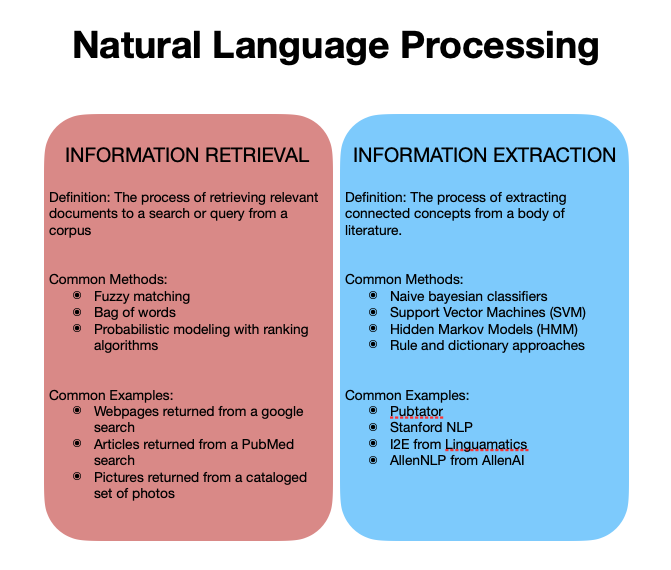
\includegraphics[height=5in]{figs/NLP_Synopsis.png}
\par\end{centering}}
\caption[Overview of Natural Language Processing Methods]{\label{nlp_synopsis} The two primary tasks of natural language processing are Information Retrieval and Extraction.}

\end{figure}

\subsection{Information Retrieval}

The task of Information Retrieval is summarized as the process of returning relevant documents based on an individual request. This task is often analogous to a google search, which returns web-pages relevant to the entered search query. Pubmed papers in the MEDLINE repository are tagged with MeSH terms that map to scientific entities and related terms. This can help narrow down paper subsets on specific topic. A query of "Bifidobacterium" quickly returns over 9,000 results where querying the MEDLINE index with the related MeSH term reduces output papers. MeSH also gives researchers the ability to add subheadings with primary query terms to further limit resulting documents. Ranking metrics can be employed to order results by importance or relevance to the search query.

\subsubsection{Ranking Algorithms}
One popular algorithm utilized by Google and Twitter is called PageRank (PR), which attempts to highlight more relevant pages with a search query\cite{page_pagerank_1998}. This works by weighting the rank of a page based on the pages that link to it using a random walk to simulate a web surfer visiting pages. The simplified algorithm is defined in equation \ref{eq:PR} with the Page Rank PR for the selected page denoted \(u\), PR for each page linking to \(u\) denoted \(v\), the set of links connecting to the page \(u\) denoted \(B(u)\), and the sum total links on page \(v\) denoted \(L(v)\). There is also a damping factor added to the equation to approximate the probability of randomly selecting another page within the subset of pages. This algorithm works well for ranking pages, ordering nodes within a graph, and in biological applications for ranking protein networks\cite{yates_pagerank_2015,engstrom_pagerank_2016}.
 \begin{equation}
  PR(u) = \sum_{v \in B(u)}{\frac{PR(v)}{L(v)}}
  \label{eq:PR}
 \end{equation}

Another algorithm utilized for ranking web-pages is the Hyperlink-Induced Topic Search HITS algorithm which calculates an authority score and a hub score \cite{mihalcea_textrank:_2004}. The authority score for a given link is calculated by summing the hub scores of pages that point to it. In contrast, each hub score is calculated by summing authority scores of pages that point to that hub. This algorithm is run at query time, which increases the time required for the database to return results.

\subsection{Information Extraction}

Literature searches often return thousands of documents, an overwhelming number for a single researcher to effectively probe before beginning research. Information extraction techniques can be employed to help researchers examine a large corpus of documents and derive meaning or extract connected concepts. Popular methods utilize Machine Learning methods, rule or dictionary based approaches, or hybrid approaches.

\subsubsection{Machine Learning Approach}

ML or statistical methods mathematically predict the entities within and the relationships they share. The problem is treated as a classification problem. Three primary techniques used are: naive bayes, Support Vector Machines (SVM), and Hidden Markov Models. 

Naive bayesian classifiers, often called the bag of words approach, are used to classify an input text with a class from a fixed set of classes. This technique is beneficial for classifying texts as belonging to a specific topic for example, distinguishing positive from negative. A pre-classified subset of training texts is required for the bayesian approach. Unfamiliar or unseen terms in the training set will be ranked with a zero, which require use of an additive algorithm to remove zero probabilities. This approach assumes word positions within the text are irrelevant to final scores, thus the informal bag-of-words name. Additionally, it is assumed that probabilities of terms within the text are independent. Both assumptions are not always true which leads to problems with sentences containing opposite classes.

Support Vector Machines are a supervised learning approach and are commonly used in NLP. They determine decision boundaries between vectors for text classification. This requires natural language text to be transformed into a vector. Standard practice is to select a maximum number of features in a training dataset, and vectorize Term Frequency, Inverse Document Frequency scores. This method builds a target vocabulary that other texts can be weighted against to determine if the threshold is high enough to cross the decision boundary. SVMs excel in classifying high-dimensional data but require labelled and balanced training datasets to perform effectively, which is a time-consuming task to manually develop when not available. An unsupervised approach can aid when supervised approaches are not optimal.

Hidden Markov Models are a common unsupervised learning method that observes a predefined number of states, or observations, and computes sequence probabilities of hidden information. This method utilizes the viterbi algorithm to decode these hidden sequence probabilities. Assigning parts of speech tags given a sentence, or input text with observed words, is a common NLP use-case. This is beneficial when limited training data is available or with specialized vocabularies. However, HMMs cannot provide assertions within text and must be combined with another method such as a rule and dictionary approach. 

\subsubsection{Rule and Dictionary Approach}

Dictionary approaches group terms into a singular value from curated synonym lists \cite{bolasco_automatic_2010}. These dictionaries can be applied on a corpus to highlight key terms within a text and classify a text based on these terms or aid researchers view groupings of terms. Pubtator is a common example that highlights chemicals, genes, pathways and phenotypes in published abstracts from the MEDLINE index \cite{wei_pubtator_2013}. Rule based approaches depend on user-chosen rules to classify texts or extract assertions. Extracting all nouns with verbs or verb phrases sandwiched in-between from assigned POS tags in a corpus, is an example of this approach. This can be informative for extracting assertions, however POS taggers must be carefully chosen based on the corpus type and are not the best choice for scientific literature.

\subsubsection{I2E}

Few NLP tools are able to extract assertions from scientific literature. Open-source tools trained on general datasets like the brown corpus work well with twitter and other sources of general knowledge but are inadequate for use on scientific literature or any body of knowledge with a highly-specialized vocabulary. I2E from Linguamatics (https://www.linguamatics.com/products/i2e) has a long history of application in the life-sciences domain and focuses on extracting assertions using a rule and dictionary approach. Assertions are extracted through queries from indexed datasets. Queries are a model of how each individual assertion is represented in the literature. These are useful on both labeled and unlabeled datasets. With labeled datasets, precision, recall, and F measures are calculated to indicate accuracy of each query. Unlabelled datasets require an iterative approach to examine the extracted assertions and refine queries. I2E provides model queries trained on MEDLINE abstracts that extract "class affects class" assertions. A "class" in I2E is a dictionary object that is used by a query to locate terms in the literature under that object. For example, all instances of \textit{Vaccinium corymbosum} are found through the NCBI taxonomy node, which contains synonyms American blueberry, highbush blueberry, and the preferred term Vaccinium corymbosum. Users will select all terms under a specific node to identify all leaf terms and synonyms from a specific dictionary, if desired. Class matches are provided confidence values using a proprietary disambiguation algorithm to filter out ambiguous matches. Benefits of using I2E include, the Graphical User Interface that is used to develop queries, quickly returned results from indexed datasets, use of many ontologies without the need to convert from various file formats, and the ability to link across separate data sources in published literature. Drawbacks include the cost to purchase a license, and the learning curve to manage indexes and ontologies into I2E specific language. Often, I2E users opt to have Linguamatics handle index creation and ontology or class parsing into I2E specific formats.

\section{Aims}

Aim 1: Develop a knowledgebase on molecular mechanisms from plants to human health by connecting siloed, sparse data from public resources and text-mined assertions.

\begin{quote}
     Given the rise in noncommunicable diseases like heart disease and diabetes, an integrated resource is necessary. This resource should combine structured and unstructured resources to connect plants to human health in a graph database. Another feature is an interface to aid users not skilled in computational biology, browse resource contents. All of this should be contained in an easy to use, easy to install, system that requires little user input. This aim will further nutrition research towards personalized solutions.
\end{quote}

Aim 2: Incorporate microbiota effects on diet and human health into the knowledgebase to identify key factors driving IBS 

\begin{quote}
    The compound effects of microbiota on diet are a required addition to the integrated resource from Aim 1. These effects should include both the effect of microbiota on phytochemicals, and the effect of phytochemicals on microbiota. Given that microbiota data is not as prevalent in abstracts, associations will be extracted from full-text articles to maximize discovery of hidden relationships. Microbiota associations will also be extracted from structured resources where available. This will provide nutritional researchers a tool to examine dietary effects on microbiota and human health. 
\end{quote}

Aim 3: Apply the knowledgebase and the methods of text-mining literature to elucidate dietary effects on SARS-CoV-2 infections.

\begin{quote}
    The SARS-CoV-2 pandemic quickly enveloped researchers, which yielded a multitude of full-text preprint publications contained in a Coronavirus specific literature set. These publications will be indexed in I2E and mined to extract the Coronavirus and associated human genes. These associations will be inserted into the knowledgebase and will be analyzed to functionally group affected human genes and pathways. Finally, plant phytochemical connections linked to the molecular mechanisms of long-COVID from coronavirus infections will be analyzed in the graph network.
\end{quote}



\chapter{THE ALIMENT TO BODILY CONDITION KNOWLEDGEBASE (ABCKB): A DATABASE CONNECTING PLANTS AND HUMAN HEALTH}

\section*{Introduction}
The growth of obesity worldwide correlates strongly with overconsumption of processed foods ~\cite{laster_beyond_2019}.This has contributed to an increase in chronic diet-related diseases like type 2 diabetes (T2D), heart disease, and some cancers ~\cite{popkin_global_2006}. Exercise and diets high in fruit, vegetables, whole grains, and nuts have been linked with healthier outcomes and reduce the risk of developing these diseases~\cite{schulze_food_2018}. Unfortunately, the specific mechanisms driving these associations are poorly understood. The Plant Pathways Elucidation Project (P2EP) was a collaboration started to uncover the mechanisms between plant-pathway products and human health~\cite{reid_need_2014}. Three questions drove this collaboration: "What do plants make," "How do they make them," and "What is their effect on human health?" The ABCkb was developed to capture the information required to answer these questions and provide researchers with a tool to build informed, nutritive hypotheses with molecular mechanisms as the linking factor between dietary plants and human health. 

These questions closely align to the recently released "2020-2030 Strategic Plan for NIH Nutrition Research.". This plan contains 4 strategic goals for further study to move closer to a precision nutrition approach including foundational research into "What do we eat and how does it affect us?" as well as understanding "How can we improve the use of food as medicine?" A cornerstone for answering these questions and the questions of the P2EP collaboration is an understanding of the mechanism of action of how our diet affects our health.

However, manually capturing this information is a difficult, time-consuming task due to scattered bodies of scientific knowledge. Currently available resources contain partial information to answer these questions, but they do not address mechanism of action. For example, the Comparative Toxicogenomics Database (CTD) connects chemicals to human health through human genes by manually curating associations between chemicals, genes, pathways and phenotypes but excludes nutritional data~\cite{davis_comparative_2019}. Specialized nutritional databases like FooDB (https://foodb.ca) and Phenol-Explorer aid researchers in estimating quantity of phytochemical content, but lack human phenotypic information~\cite{rothwell_phenol-explorer_2013}. NutriChem was developed to bridge the gap between plant-based nutrition and human disease through the chemicals contained in those plants, but does not contain gene-chemical associations, a key part of the driving molecular mechanisms between diet and human health~\cite{jensen_nutrichem_2015}. While a small proportion of assertions are in available databases, others are hidden in published research and can only be extracted through extensive reading or by natural language processing (NLP) the literature. Given the rise in diet-related diseases, and the pursuit of personalized nutrition, an integrated resource to develop nutritive hypotheses is necessary.

\section*{Main Text}

We have developed the Aliment to Bodily Condition Knowledgebase (ABCkb) to address the gap of connecting plant compounds to human indications through their mechanism of action. The ABCkb integrates multiple resources for building informed hypotheses with molecular mechanisms as the linking factor between dietary plants and human health. To accomplish this, the ABCkb uses both structured and unstructured data sources (Fig.~\ref{fig_2_1}). The structured resources are publicly accessible, curated databases and the unstructured data is in the form of Medline abstracts. Since this data, composed of entities and relationships or nodes and edges, composes a graphical network, we extracted, transformed, and then loaded into a Neo4j graph database. To help users begin discovering these nutritive connections, the knowledgebase is available on GitHub and a simplified online web interface.

\begin{figure}[!h]
{\begin{centering}
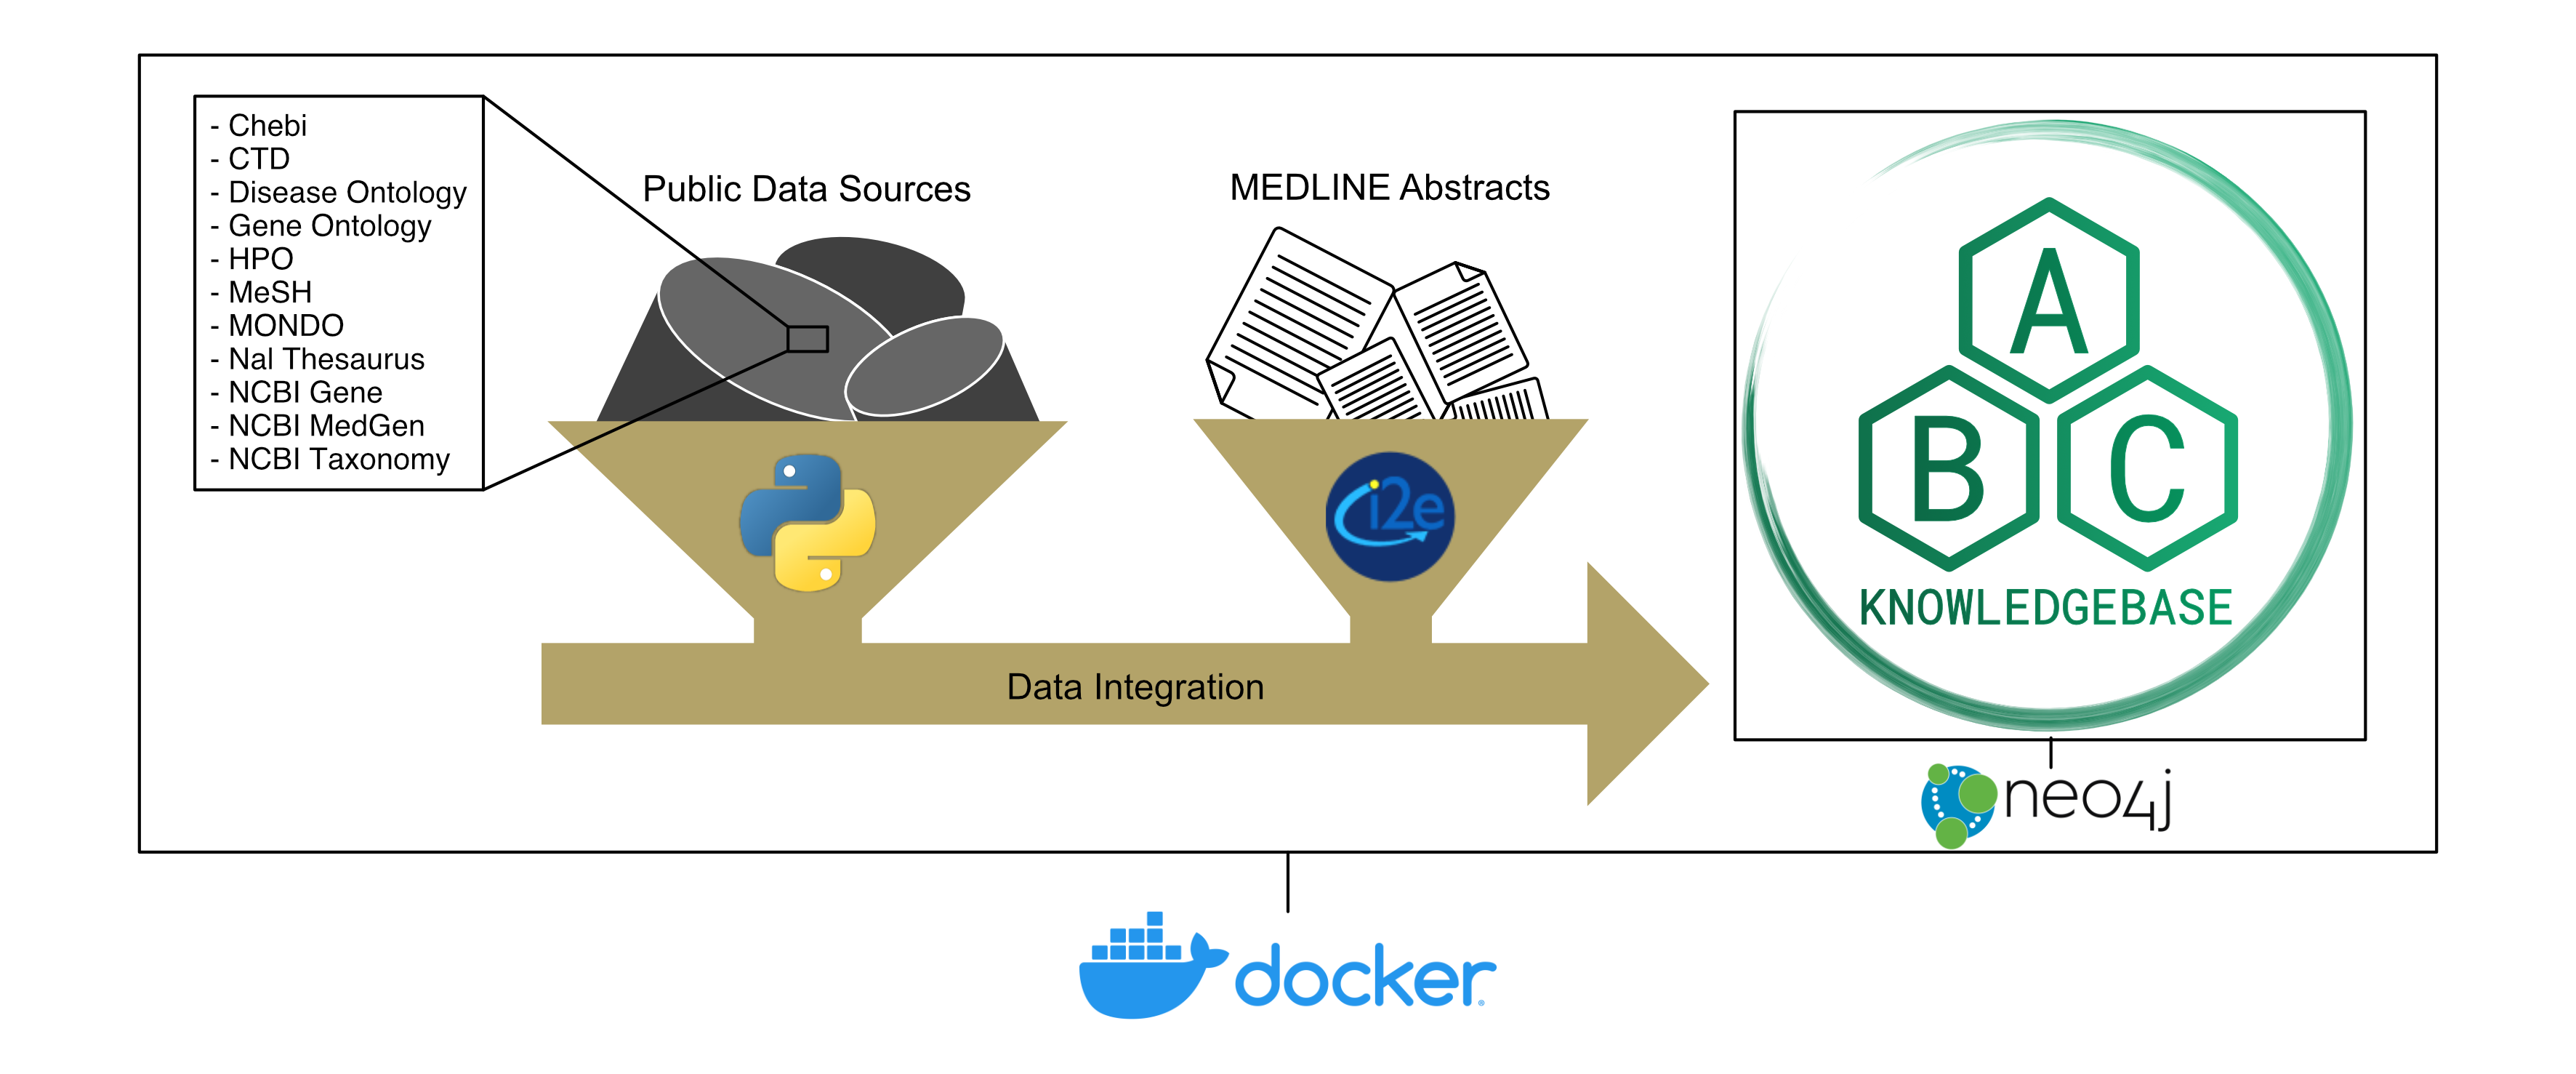
\includegraphics[height=2.5in]{figs/Fig_2_1.png}
\par\end{centering}}
\caption[ABCkb Pipeline Overview]{\label{fig_2_1} The architectural diagram of our Knowledgebase shows the various tools and resources utilized to generate the database.}

\end{figure}

\subsection*{Structured resource collection}
Structured data from 11 resources (Fig.~\ref{fig_2_2}) produce five major node types (Plant, Chemical, Gene, Pathway, Phenotype) in a Neo4j graph database. Connections, or edges between these nodes are provided by both structured data, and unstructured MEDLINE Abstracts through NLP. The ABCkb utilizes three types of structured data sources: ontologies, structured vocabularies, and databases.


\begin{figure}[!h]
{\begin{centering}
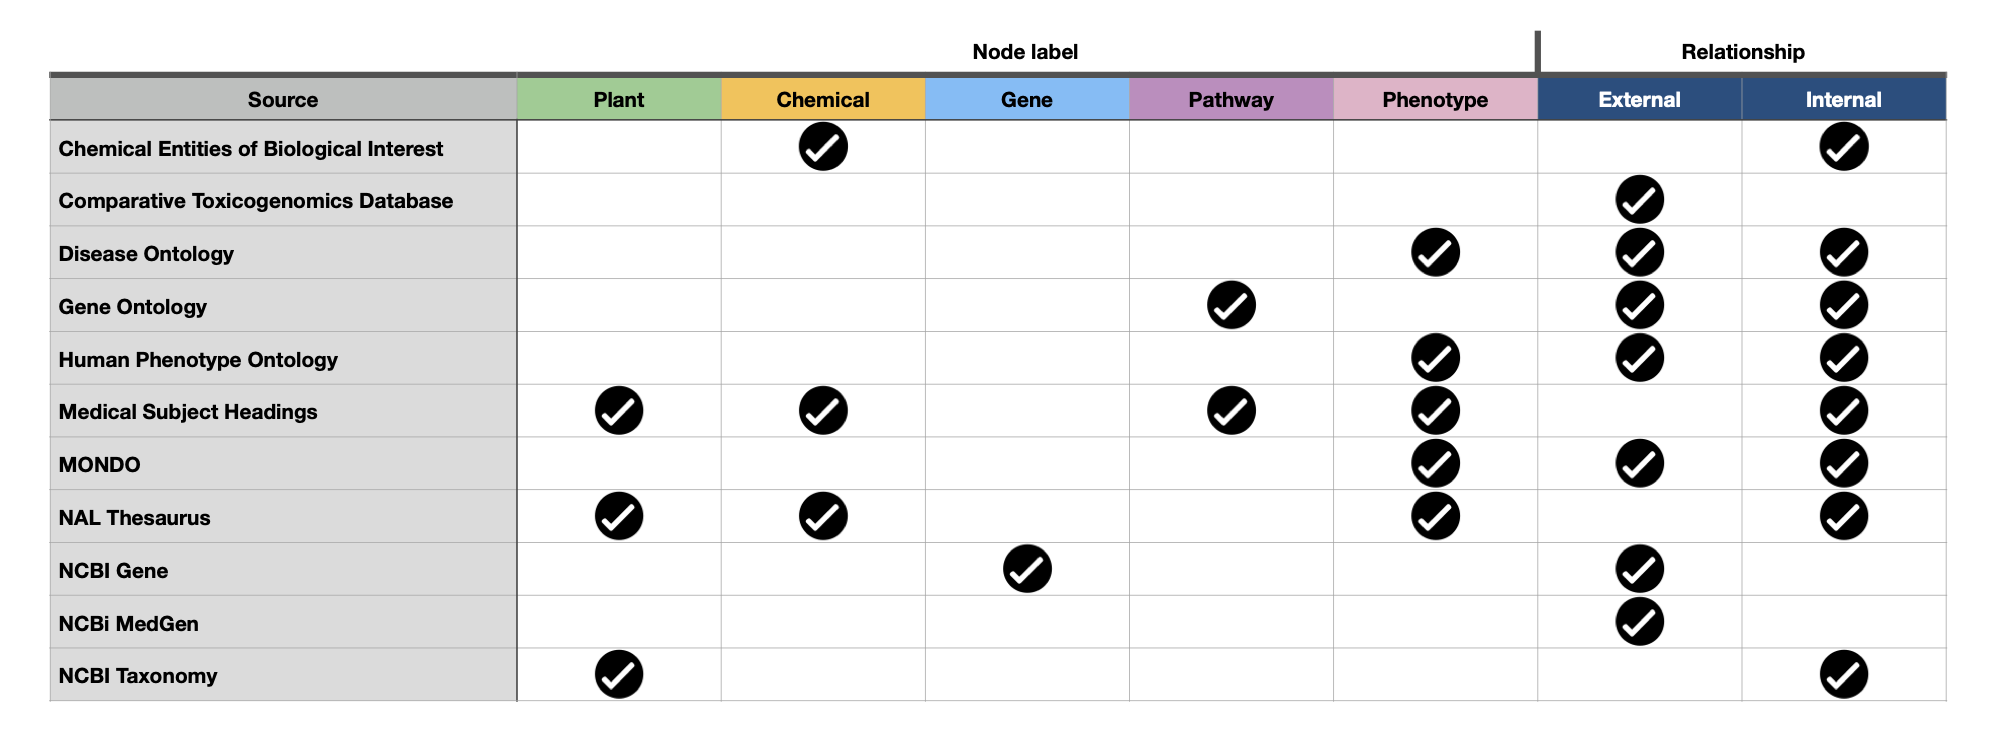
\includegraphics[height=2in]{figs/Fig_2_2.png}
\par\end{centering}}
\caption[ABCkb data sources]{\label{fig_2_2} Data from each source is transformed into one of the 5 labels and may provide external and internal references to nodes within the knowledgebase. The CTD provides manually curated references between labels with no original node labels}

\end{figure}

\subsubsection*{Ontologies and Structured Vocabularies}
The ontologies and structured vocabularies create well-controlled edges between chemicals, pathways, and phenotypes. The Chemical Entities of Biological Interest provide chemical nodes and semantic connections (edges) between chemicals~\cite{hastings_chebi_2016}. Genes are grouped into pathways from the Gene Ontology resource~\cite{ashburner_gene_2000,the_gene_ontology_consortium_gene_2019}. Human phenotypes are represented from three sources. The Disease Ontology categorizes human diseases with phenotypic characteristics~\cite{schriml_human_2019}. The Human Phenotype Ontology provides phenotypic abnormalities not found within the Disease Ontology which allows researchers to focus on specific phenotypic symptoms and the associated molecular mechanisms~\cite{kohler_expansion_2019}. Finally, the MONDO Disease Ontology was used to collapse similar phenotype nodes from multiple sources using their source identifiers ~\cite{mungall_monarch_2017}. The Medical Subject Headings resource provided nodes and connections for all major labels with the exception of Genes~\cite{noauthor_medical_nodate}. Additional plant, chemical, and phenotype nodes were extracted from the National Agricultural Library Thesaurus~\cite{noauthor_agricultural_nodate}. Terms from different ontologies or vocabularies with the same identifiers are collapsed into the same node. All other nodes are left separate to retain their hierarchical relationships.

\subsubsection*{Databases}
Several databases were utilized to increase molecular mechanisms from plant to human disease in the ABCkb. The Comparative Toxicogenomics Database added over 7.4 million manually curated edges between chemicals, genes, pathways, and phenotype nodes~\cite{davis_comparative_2019}. We utilized three public databases from The National Center for Biotechnology Information. All plants under the Embryophyta clade from the NCBI Taxonomy database produced plant nodes and phylogenetic relationships between plants~\cite{federhen_ncbi_2012,sayers_genbank_2019}. The Gene database provided gene names, types, and synonyms~\cite{brown_gene_2015}. Finally, additional edges were added utilizing NCBI gene nodes and MONDO phenotypes were extracted from the NCBI MedGen database~\cite{halavi_medgen_2018}. The compendium of structured data sources provide many of the node and edges connecting plants to disease. However, unstructured literature contains informative relationships not contained within these sources, leaving many gaps in our understanding.

\subsection*{Unstructured NLP collection}
To uncover relationships in literature, elucidate molecular mechanisms, and answer the three questions of the P2EP, we mined the literature using Linguamatics' I2E NLP text mining platform (https://www.linguamatics.com/products/i2e). This platform utilizes ontologies and structured vocabularies to transform unstructured text into structured assertions (nodes and edges).
% \paragraph*{Sub-sub-sub heading for section}

\subsubsection*{Natural Language Processing of MEDLINE Abstracts}
The I2E platform employs a graphical user interface for NLP query development, where each query extracts a set of subjects, objects, and predicates, or relationships from user-specified ontologies and structured vocabularies. From published abstracts, and titles extracted from MEDLINE in May, 2019, NLP queries were developed with I2E for each of the 4 steps (plant to chemical, chemical to gene, gene to pathway, pathway to phenotype) with an additional query from genes to phenotypes. All I2E assertions generated are provided to users of the ABCkb as source files and are parsed when the graph database is built.

\subsection*{Statistics and application}
Extracted public data sources generated over 957,000 nodes with over 11 million edge relationships. NLP results from I2E queries make up 1.26 million of the overall relationship count, of which 1.25 million relationships were novel, not from structured public data sources. Figure ~\ref{kb_stats} gives a visual presentation of (a) the relative number of each node type and their source, (b) the edge relationships from each source and (c) the relative comparison of edge relationship types between each type of node. 

\begin{figure}[!h]
{\begin{centering}
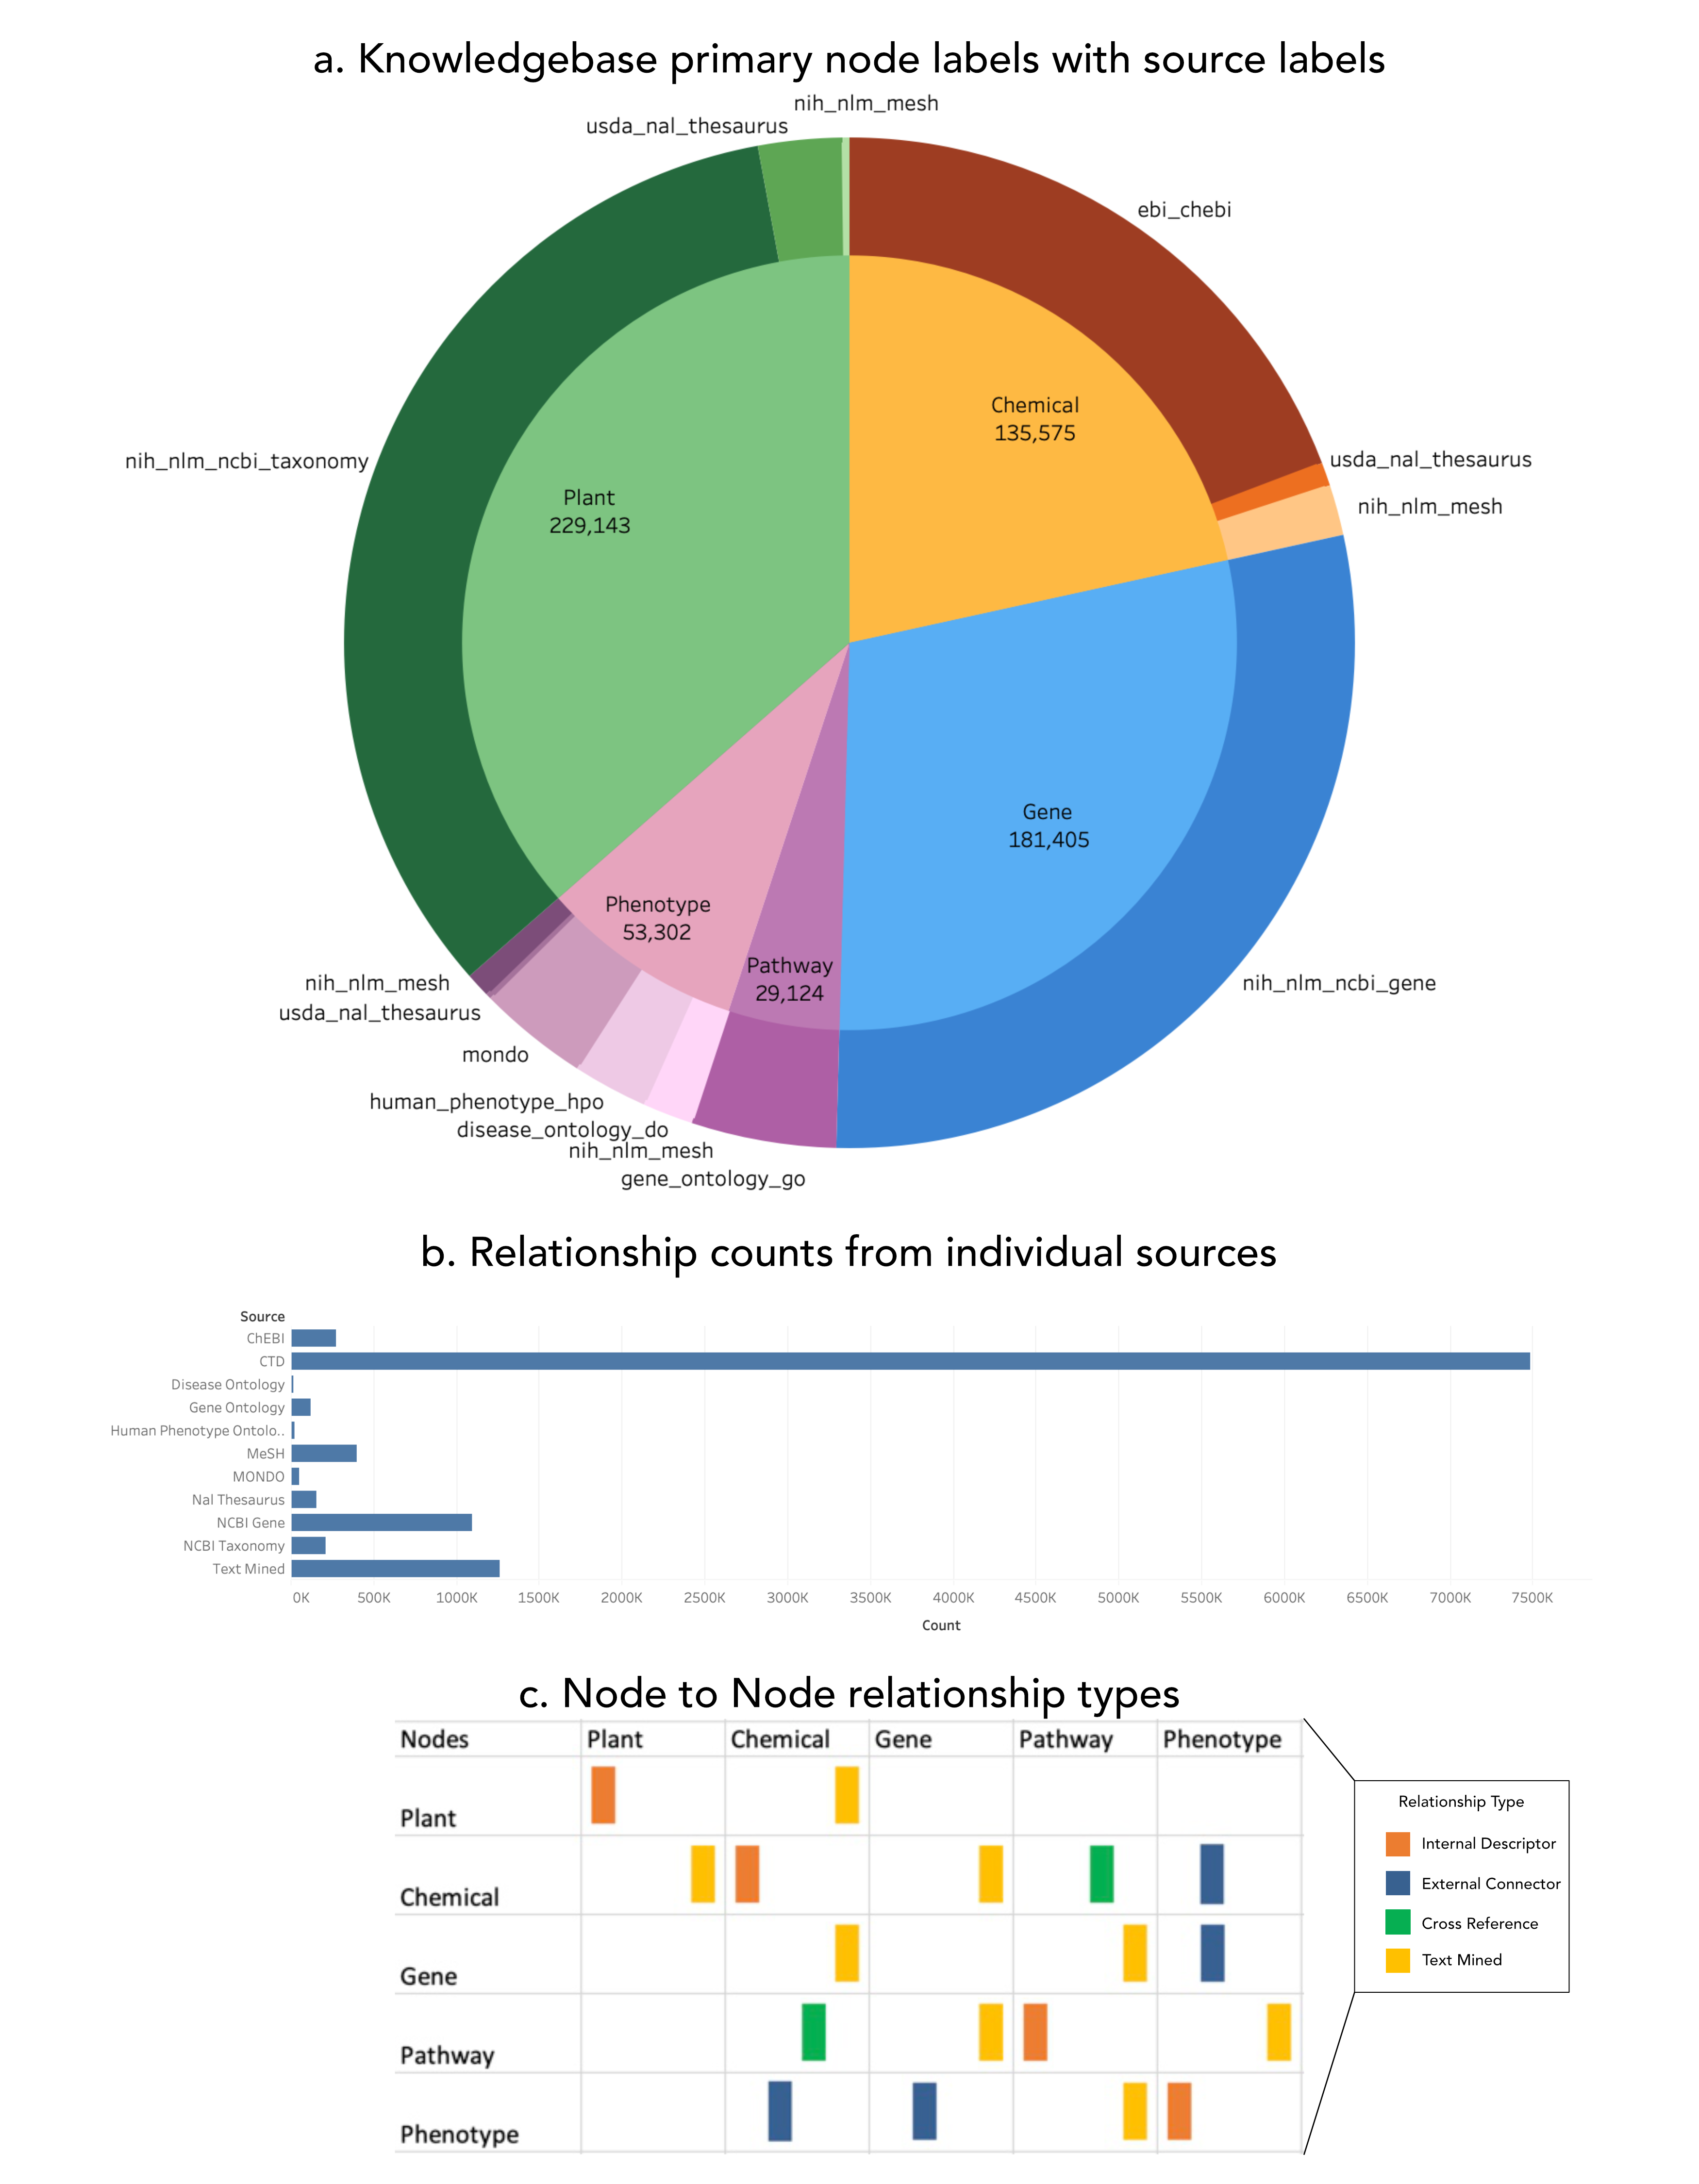
\includegraphics[height=7.5in]{figs/Fig_2_3.png}
\par\end{centering}}
\caption[ABCkb node and relationship statistics]{\label{kb_stats} a. The pie chart shows primary labels indicated by color with named secondary (source) labels, shaded and sized by proportion of total nodes in the knowledgebase. b. The sum of relationship counts for each source is indicated by the bar chart. c. Relative relationship counts indicated from node-node in rows, columns in a bar chart in order by type (Internal Descriptor, External Connector, Cross Reference, and Text Mined)}
\end{figure}

This collection of nodes and edge relationships forming semantic triples, naturally forms a biological network of knowledge that is best stored in a graph database like Neo4j. Chaining these triples together in the ABCkb highlights connections between dietary plants and human phenotypes that would otherwise go unseen if left in their original sources, particularly unstructured literature sources. The intention of the knowledgebase is for information in the network to flow from plants to phenotypes/disease indications, however, assertions are maintained in both directions, which allows for query flexibility of relationships between any nodes. Start and end node types are not enforced which allows queries from any point, to any point. All associations are kept along with references to the original source allowing the user to evaluate potential inconsistencies using the original evidence. To explore the database and discover connections, users have two choices. One, use the online interface (available at https://abckb.charlotte.edu). Otherwise, download from GitHub and build the database on a local machine which can then be queried in the Neo4j interface, or on the command line. A prebuilt data folder with the neo4j database is also available~\cite{trautman_aliment_2021}.

The provided user-friendly interface aids users unfamiliar with Neo4j query language (Cypher) to browse the contents within and examine nutritive connections (Fig.~\ref{kb_interface}). On the home page, users are provided a search box to enter in a search term. This scans the nodes in the knowledgebase and returns results ranked by similarity to search term. Users can select nodes and continue to build a query to any end point within the knowledgebase (plant, chemical, gene, pathway, or phenotype). Running the query scans the database for all paths to the selected end point and returns them to the user, which are available to download. Additionally, a Cypher query is available to users that can be used in the built in Neo4j interface or the terminal for further exploration.

\begin{figure}[!h]
{\begin{centering}
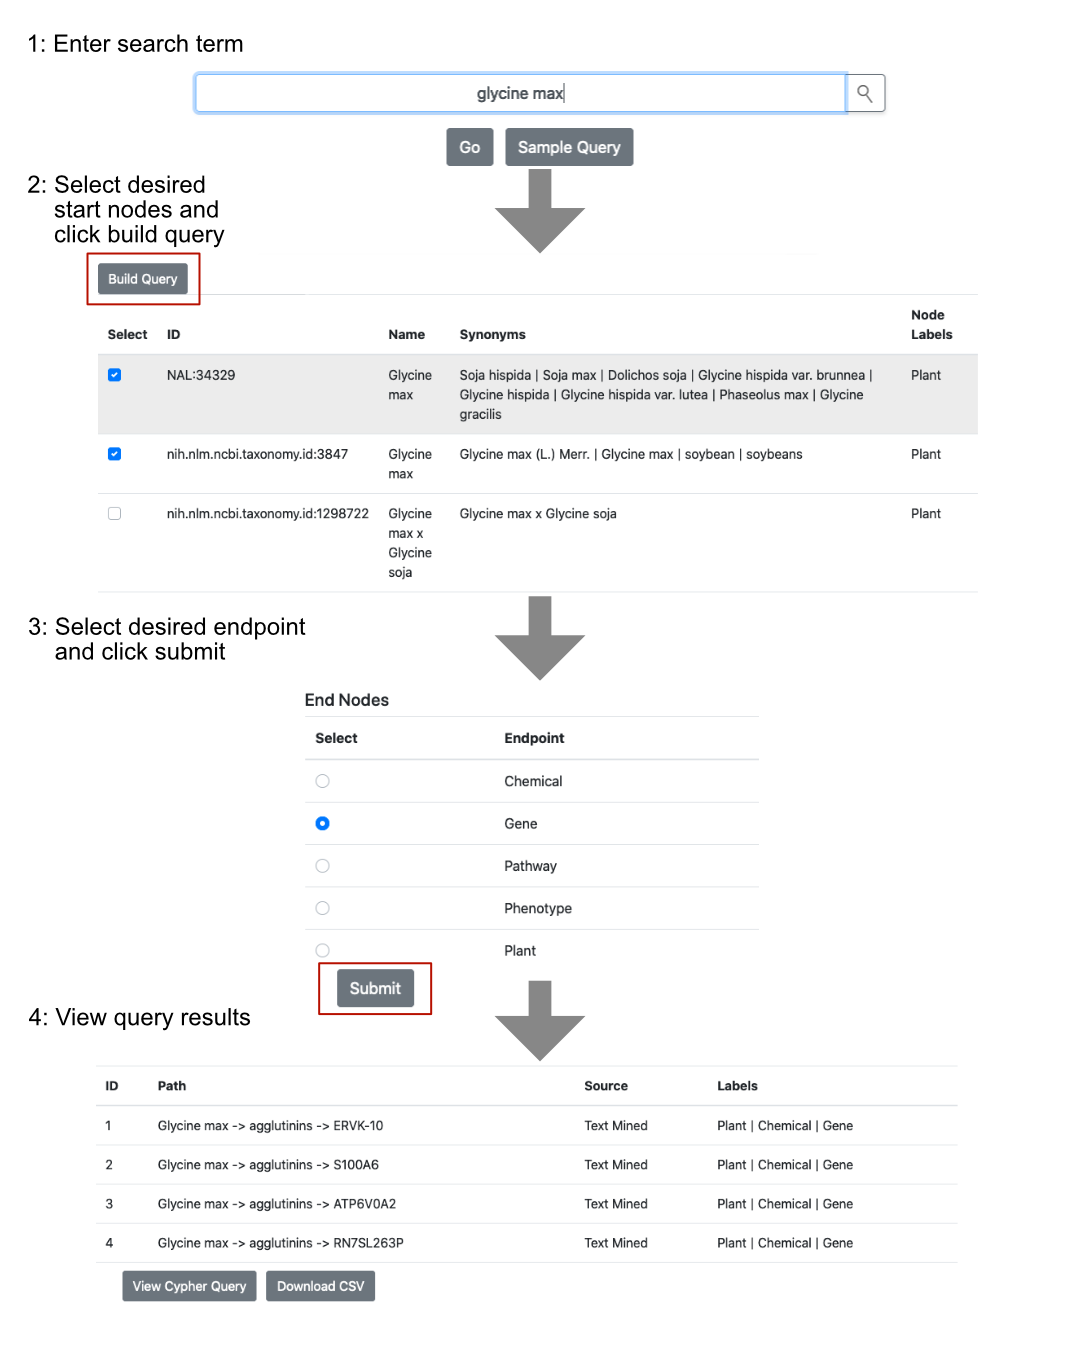
\includegraphics[height=7in]{figs/Fig_2_4.png}
\par\end{centering}}
\caption[Browsing the ABCkb Interface]{\label{kb_interface} There are 4 primary steps to browsing using the provided interface. Once the query endpoint is selected and the user clicks submit, they have the option of downloading all results as a csv, or viewing the Cypher query.}
\end{figure}

\subsubsection*{Oat and Type 2 Diabetes}

To demonstrate how the ABCkb connects dietary plants to separate human indications through molecular mechanisms, a graph was created in the ABCkb, through the Neo4j browser, depicting the diet-disease network between \textit{Avena sativa}, T2D, and heart failure (Fig~\ref{av_2_diab}). Connections from the CTD indicate genes commonly associated with cholesterol and heart failure. However, text-mining indicates that consumption of oats affects cholesterol levels in the body, which is associated with the gene HSD11B1 that affects lipid metabolic processes with both positive and negative impacts on the incidence of T2D. These relationships are due to the presence of beta-glucan in oat grains. Consumption of beta-glucan-containing oat can help lower LDL cholesterol~\cite{wolever_oat_2016}. The cholesterol lowering effects of oat can also be attributed to the presence of certain lipids and proteins~\cite{guo_cholesterol-lowering_2014}. The proteins in oat with low lysine-arginine and methionine-glycine ratios contribute to lower total cholesterol and LDL cholesterol levels. Hypocholesterolemic properties of oat cannot simply be attributed to one factor, but a combination of many, including oleic acid, vitamin E, and plant sterols~\cite{guo_cholesterol-lowering_2014}.

\begin{figure}[!h]
{\begin{centering}
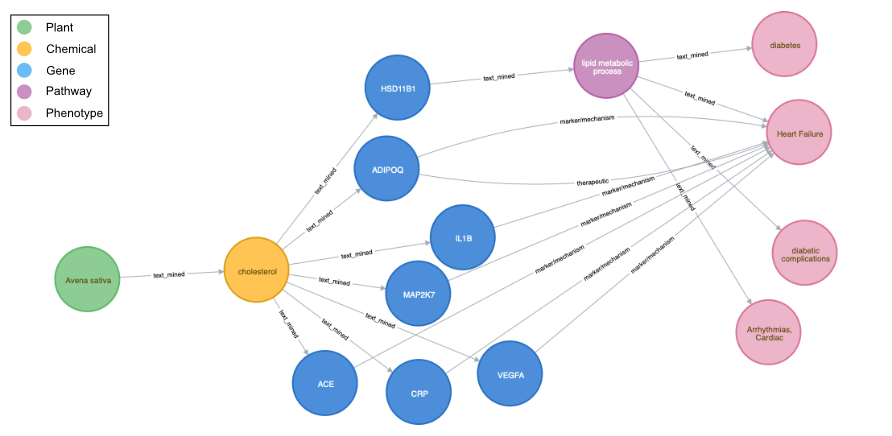
\includegraphics[height=2.7in]{figs/Fig_2_5.png}
\par\end{centering}}
\caption[Visualizing the results of \textit{Avena sativa} to diabetes and heart failure via Hydroxysteroid 11-Beta Dehydrogenase 1.]{\label{av_2_diab} This meta-path highlights the connectivity between oats, diabetes, and heart failure through the gene HSD11B1 from the ABCkb.}

% Generated with:
% MATCH p=(:Plant {source_id:"nih.nlm.ncbi.taxonomy.id:4498"})-->
%        (:Chemical {name:"cholesterol"})-->
%        (:Gene {name:"HSD11B1"})-->
%        (:Pathway {source_id:"GO:0006629"})-->
%        (ph:Phenotype) 
% WHERE ph.name =~ "diabet.*" OR 
%         ph.name =~ ".*eart.*" OR 
%         ph.name =~ ".*ardiac.*"
% RETURN p
\end{figure}

T2D patients frequently have abnormal levels of many different lipids, as well as abnormal qualities to these lipids, for example, T2D patients experience normal or slightly elevated LDL cholesterol with increased LDL oxidation and glycation~\cite{verges_new_2005}. Dyslipidemia in T2D patients is associated with cardiovascular disease ~\cite{pokharel_prevalence_2017,shahwan_prevalence_2019}. This creates an elevated risk for cardiovascular diseases including atherosclerosis, and dislipidemia may play a role in these risks~\cite{shahwan_prevalence_2019}. In the graph, HSD11B1 is the human gene connecting this relationship. HSD11B1 expression is increased in adipose tissues of obese individuals~\cite{paulsen_11beta-hsd_2007}. Dysregulation of HSD11B1 is associated with an imbalance of glucocorticoid in adipose tissues, glucose imbalance, and visceral fat accumulation~\cite{dammann_expression_2019}. These factors contribute to metabolic syndrome, which puts patients at a higher risk for cardiac diseases~\cite{turek_gender-dependent_2014}. Various SNPs in HSD11B1 have associations with T2D, metabolic syndrome, and hypertension~\cite{nair_11beta-hydroxysteroid_2004,gambineri_combination_2011,freedman_distribution_2001,goff_insulin_2005}. 

Due to the established relationship between oat beta-glucans, cholesterol, and weight, the connection to T2D is logical~\cite{wolever_oat_2016,dammann_expression_2019}. Decreased weight, specifically visceral fat in the abdomen, would result in reduced expression of HSD11B1, which would improve regulation of cortisol. Further examination of the oat - cholesterol - HSD11B1 relationship could be very informative to both patients and doctors in making more informed dietary choices and reducing the risk of developing T2D. This example demonstrates the ABCkb ability to connect seemingly separate conditions through the molecular mechanistic links within.

\subsection*{Discussion}

The ABCkb integrates structured and unstructured resources in a network that connects plants to human disease through molecular mechanisms. This reduces the time required to manually connect these links through each individual resource. Additionally, knowledge discovery is aided by the development of a user-friendly interface. All of these components provide precision nutrition a path to better understand the mechanisms behind diet-related conditions. The ABCkb is available from the interface (https://abckb.charlotte.edu).

\section*{Limitations}

\begin{itemize}
\item Microbiota contributions to diet and human disease. Bacteria within the gut are known to affect disease both through the production of metabolites and the conversion of plant phytochemicals. In addition, gut bacteria are affected by diet. Future implementations of the ABCkb will contain microbiota associations to enhance precision nutrition hypotheses.
\item Mining abstracts versus full text. Abstracts contain valuable associations, however associations full text articles would provide a greater number of associations.
\item Incorporating genomic data. Precision nutrition hypotheses and treatment plans will depend on patient genomic data, to provide optimal dietary solutions for each individual. Future versions of the ABCkb should incorporate human genomic data.
\end{itemize}


% \section{}

% We have developed the Aliment to Bodily Condition Knowledgebase (ABCkb) to address the gap of connecting plant compounds to human indications through their mechanism of action. The ABCkb integrates multiple resources for building informed hypotheses with molecular mechanisms as the linking factor between dietary plants and human health. To accomplish this, the ABCkb uses both structured and unstructured data sources (Figure.~\ref{fig_2_1}). The structured resources are publicly accessible, curated databases and the unstructured data is in the form of Medline abstracts. Data is extracted, transformed, and then loaded into a Neo4j database. To help users begin discovering easily, the knowledgebase is available as a Docker instance. Additionally, an interface is provided to aid discovery of nutritive connections.

% \begin{figure}[!h]
% {\begin{centering}
% 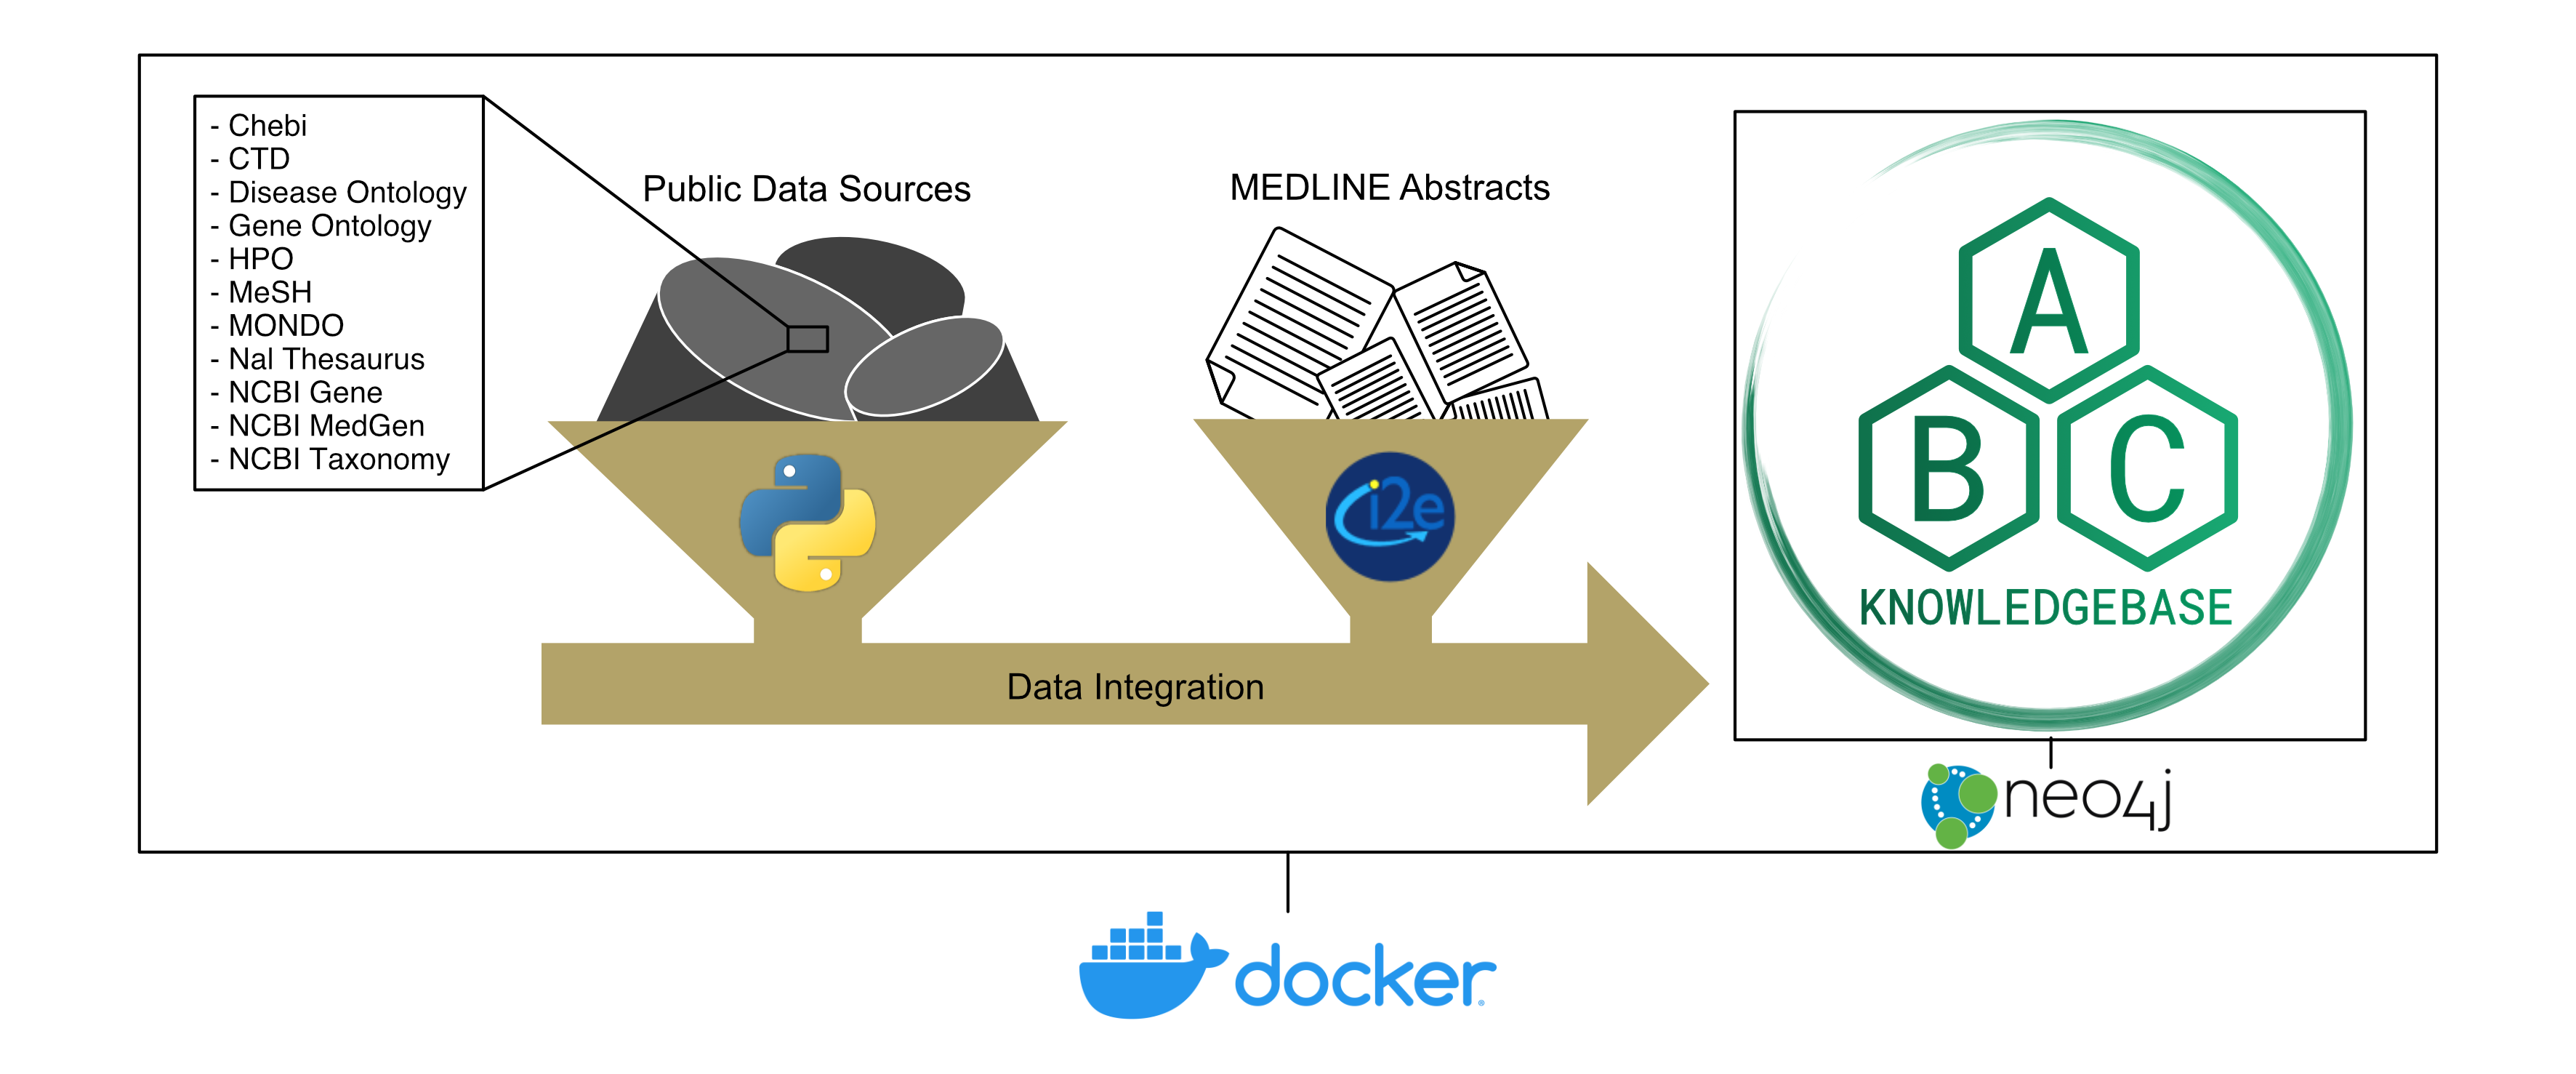
\includegraphics[height=2in]{figs/Fig_2_1.png}
% \par\end{centering}}
% \caption[ABCkb Pipeline Overview]{\label{fig_2_1} The architectural diagram of our Knowledgebase shows the various tools and resources utilized to generate the database.}

% \end{figure}

% \subsection{Structured resource collection}
% Structured data from 11 resources (Figure.~\ref{fig_2_2}) produce five major labels (Plant, Chemical, Gene, Pathway, Phenotype) in a Neo4j graph database. Connections between these labels are provided by both structured data, and unstructured MEDLINE Abstracts through NLP. The ABCkb utilizes three types of structured data sources: ontologies, structured vocabularies, and databases.


% \begin{figure}[!h]
% {\begin{centering}
% 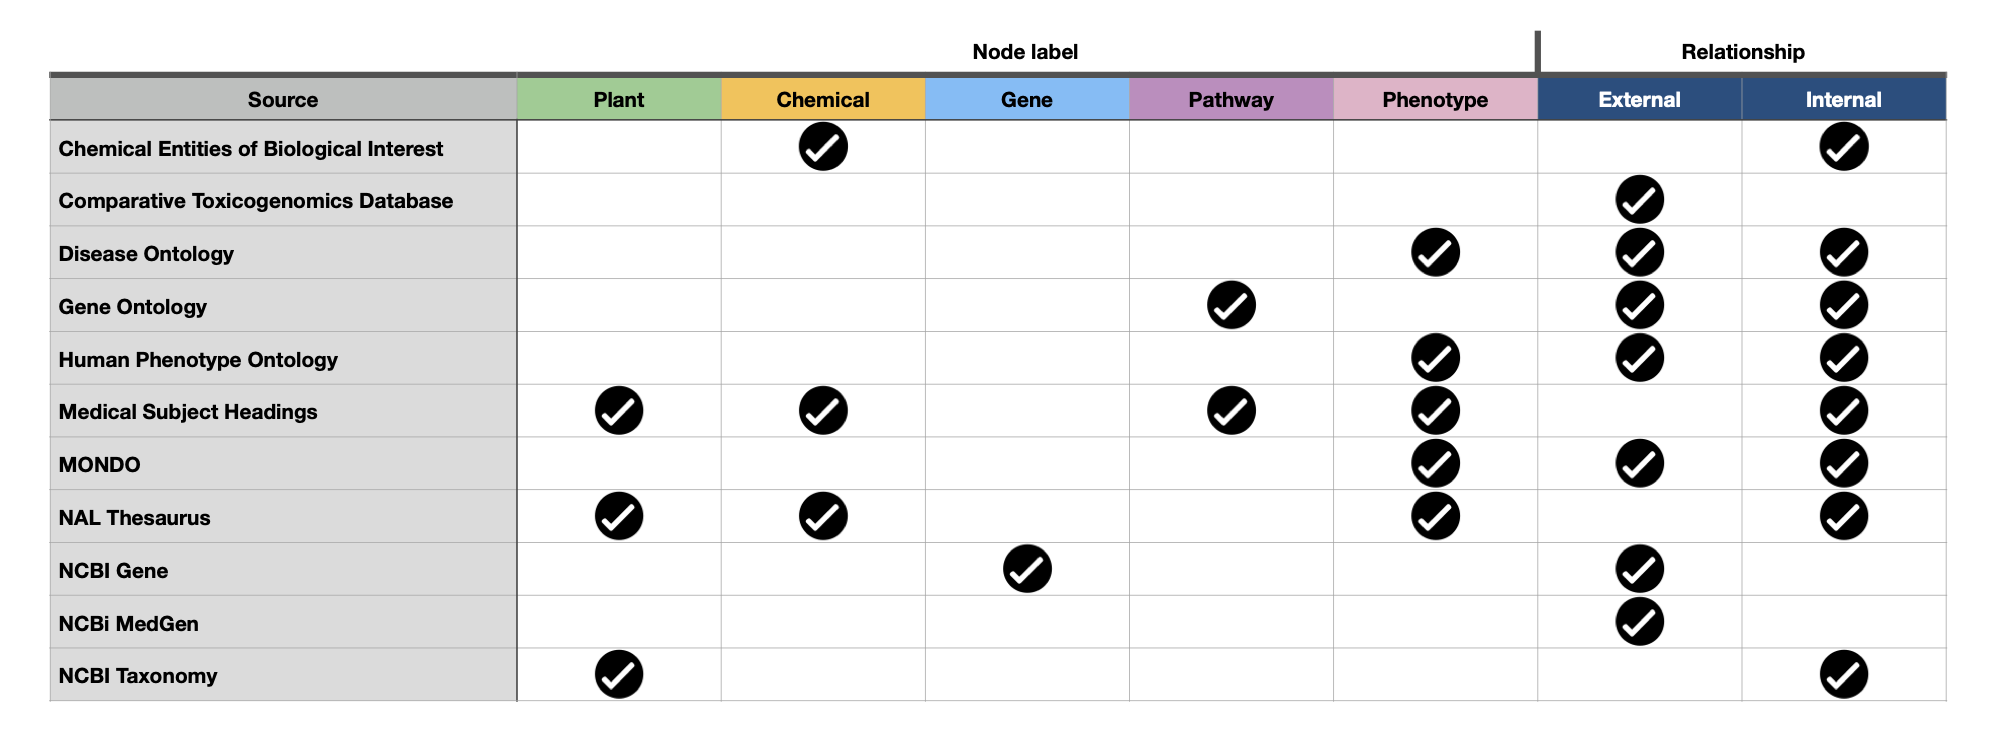
\includegraphics[height=2in]{figs/Fig_2_2.png}
% \par\end{centering}}
% \caption[ABCkb data sources]{\label{fig_2_2} Data from each source is transformed into one of the 5 labels and may provide external and internal references to nodes within the knowledgebase. The CTD provides manually curated references between labels with no original node labels.}

% \end{figure}


% \subsubsection{Ontologies and Structured Vocabularies}
% The ontologies and structured vocabularies enable well-controlled links between chemicals, pathways, and phenotypes. The Chemical Entities of Biological Interest provide chemical nodes and semantic connections between chemicals~\cite{hastings_chebi_2016}. Genes are grouped into pathways from the Gene Ontology resource~\cite{ashburner_gene_2000,thegeneontologyconsortium_gene_2019}. Human phenotypes are represented from three sources. The Disease Ontology categorizes human diseases with phenotypic characteristics~\cite{schriml_human_2019}. The Human Phenotype Ontology provides phenotypic abnormalities not found within the Disease Ontology which allows researchers to focus on specific phenotypic symptoms and the associated molecular mechanisms~\cite{kohler_expansion_2019}. Finally, the MONDO Disease Ontology was used to connect phenotype nodes from multiple sources ~\cite{mungall_monarch_2017}. The Medical Subject Headings resource provided nodes and connections for all major labels with the exception of Genes~\cite{noauthor_medical_nodate}. Additional plant, chemical, and phenotype nodes are extracted from the National Agricultural Library Thesaurus~\cite{noauthor_agricultural_nodate}. Both NAL and MeSH are general sources of knowledge for their domains, provide a wide range of term synonyms, and are used in NLP queries to extract associations from literature and connect extracted associations in the ABCkb. Incorporation of these sources expands the diet to disease connections within the ABCkb

% \subsubsection{Databases}
% Several databases were utilized to increase molecular mechanisms from plant to human disease in the ABCkb. The Comparative Toxicogenomics database was brought in for over 7.4 million manually curated associations between chemicals, genes, pathways, and phenotypes~\cite{davis_comparative_2019}. The National Center for Biotechnology Information provides various databases available to the public of which, we utilized three. All plants under the Embryophyta clade from the NCBI Taxonomy database produce plant nodes and phylogenetic relationships between plants~\cite{federhen_ncbi_2012,sayers_genbank_2019}. The Gene database provides gene names, types, and synonyms~\cite{brown_gene_2015}. Finally, relationships between NCBI gene nodes and MONDO phenotypes were extracted from the NCBI MedGen database~\cite{halavi_medgen_2018}. The compendium of structured data sources provide molecular pathways from diet to disease. However, unstructured literature contains informative relationships not contained within these sources.

% \subsection{Unstructured NLP collection}
% To uncover associations in literature, elucidate molecular mechanisms, and answer the three questions of the P2EP, we mined the literature using Linguamatics' I2E NLP text mining platform. This platform utilizes ontologies and structured vocabularies to transform unstructured text into structured assertions.
% % \paragraph*{Sub-sub-sub heading for section}

% \subsubsection{Natural Language Processing of MEDLINE Abstracts}
% The I2E platform employs a graphical user interface to aid NLP query development, where each query extracts a set of subjects, objects, and predicates from user-specified ontologies and structured vocabularies. From published abstracts, and titles extracted from MEDLINE in May, 2019, NLP queries were developed with I2E for each of the 4 steps (plant to chemical, chemical to gene, gene to pathway, pathway to phenotype) with an additional query from genes to phenotypes. All I2E assertions generated are provided to users of the ABCkb as source files and are parsed when the graph database is built.

% \subsection{Statistics and application}
% Extracted public data sources generated over 957,000 nodes with over 11 million relationships. NLP results from I2E queries make up 1.26 million of the overall relationship count, with 1.25 million novel relationships not from structured public data sources. There are a total of 14 node labels, with the primary focus on 5 labels forming a direct path from plants to human health (Figure.~\ref{kb_stats}a), and 29 relationship types from 11 different sources (Figure.~\ref{kb_stats}b).

% \begin{figure}[!h]
% {\begin{centering}
% 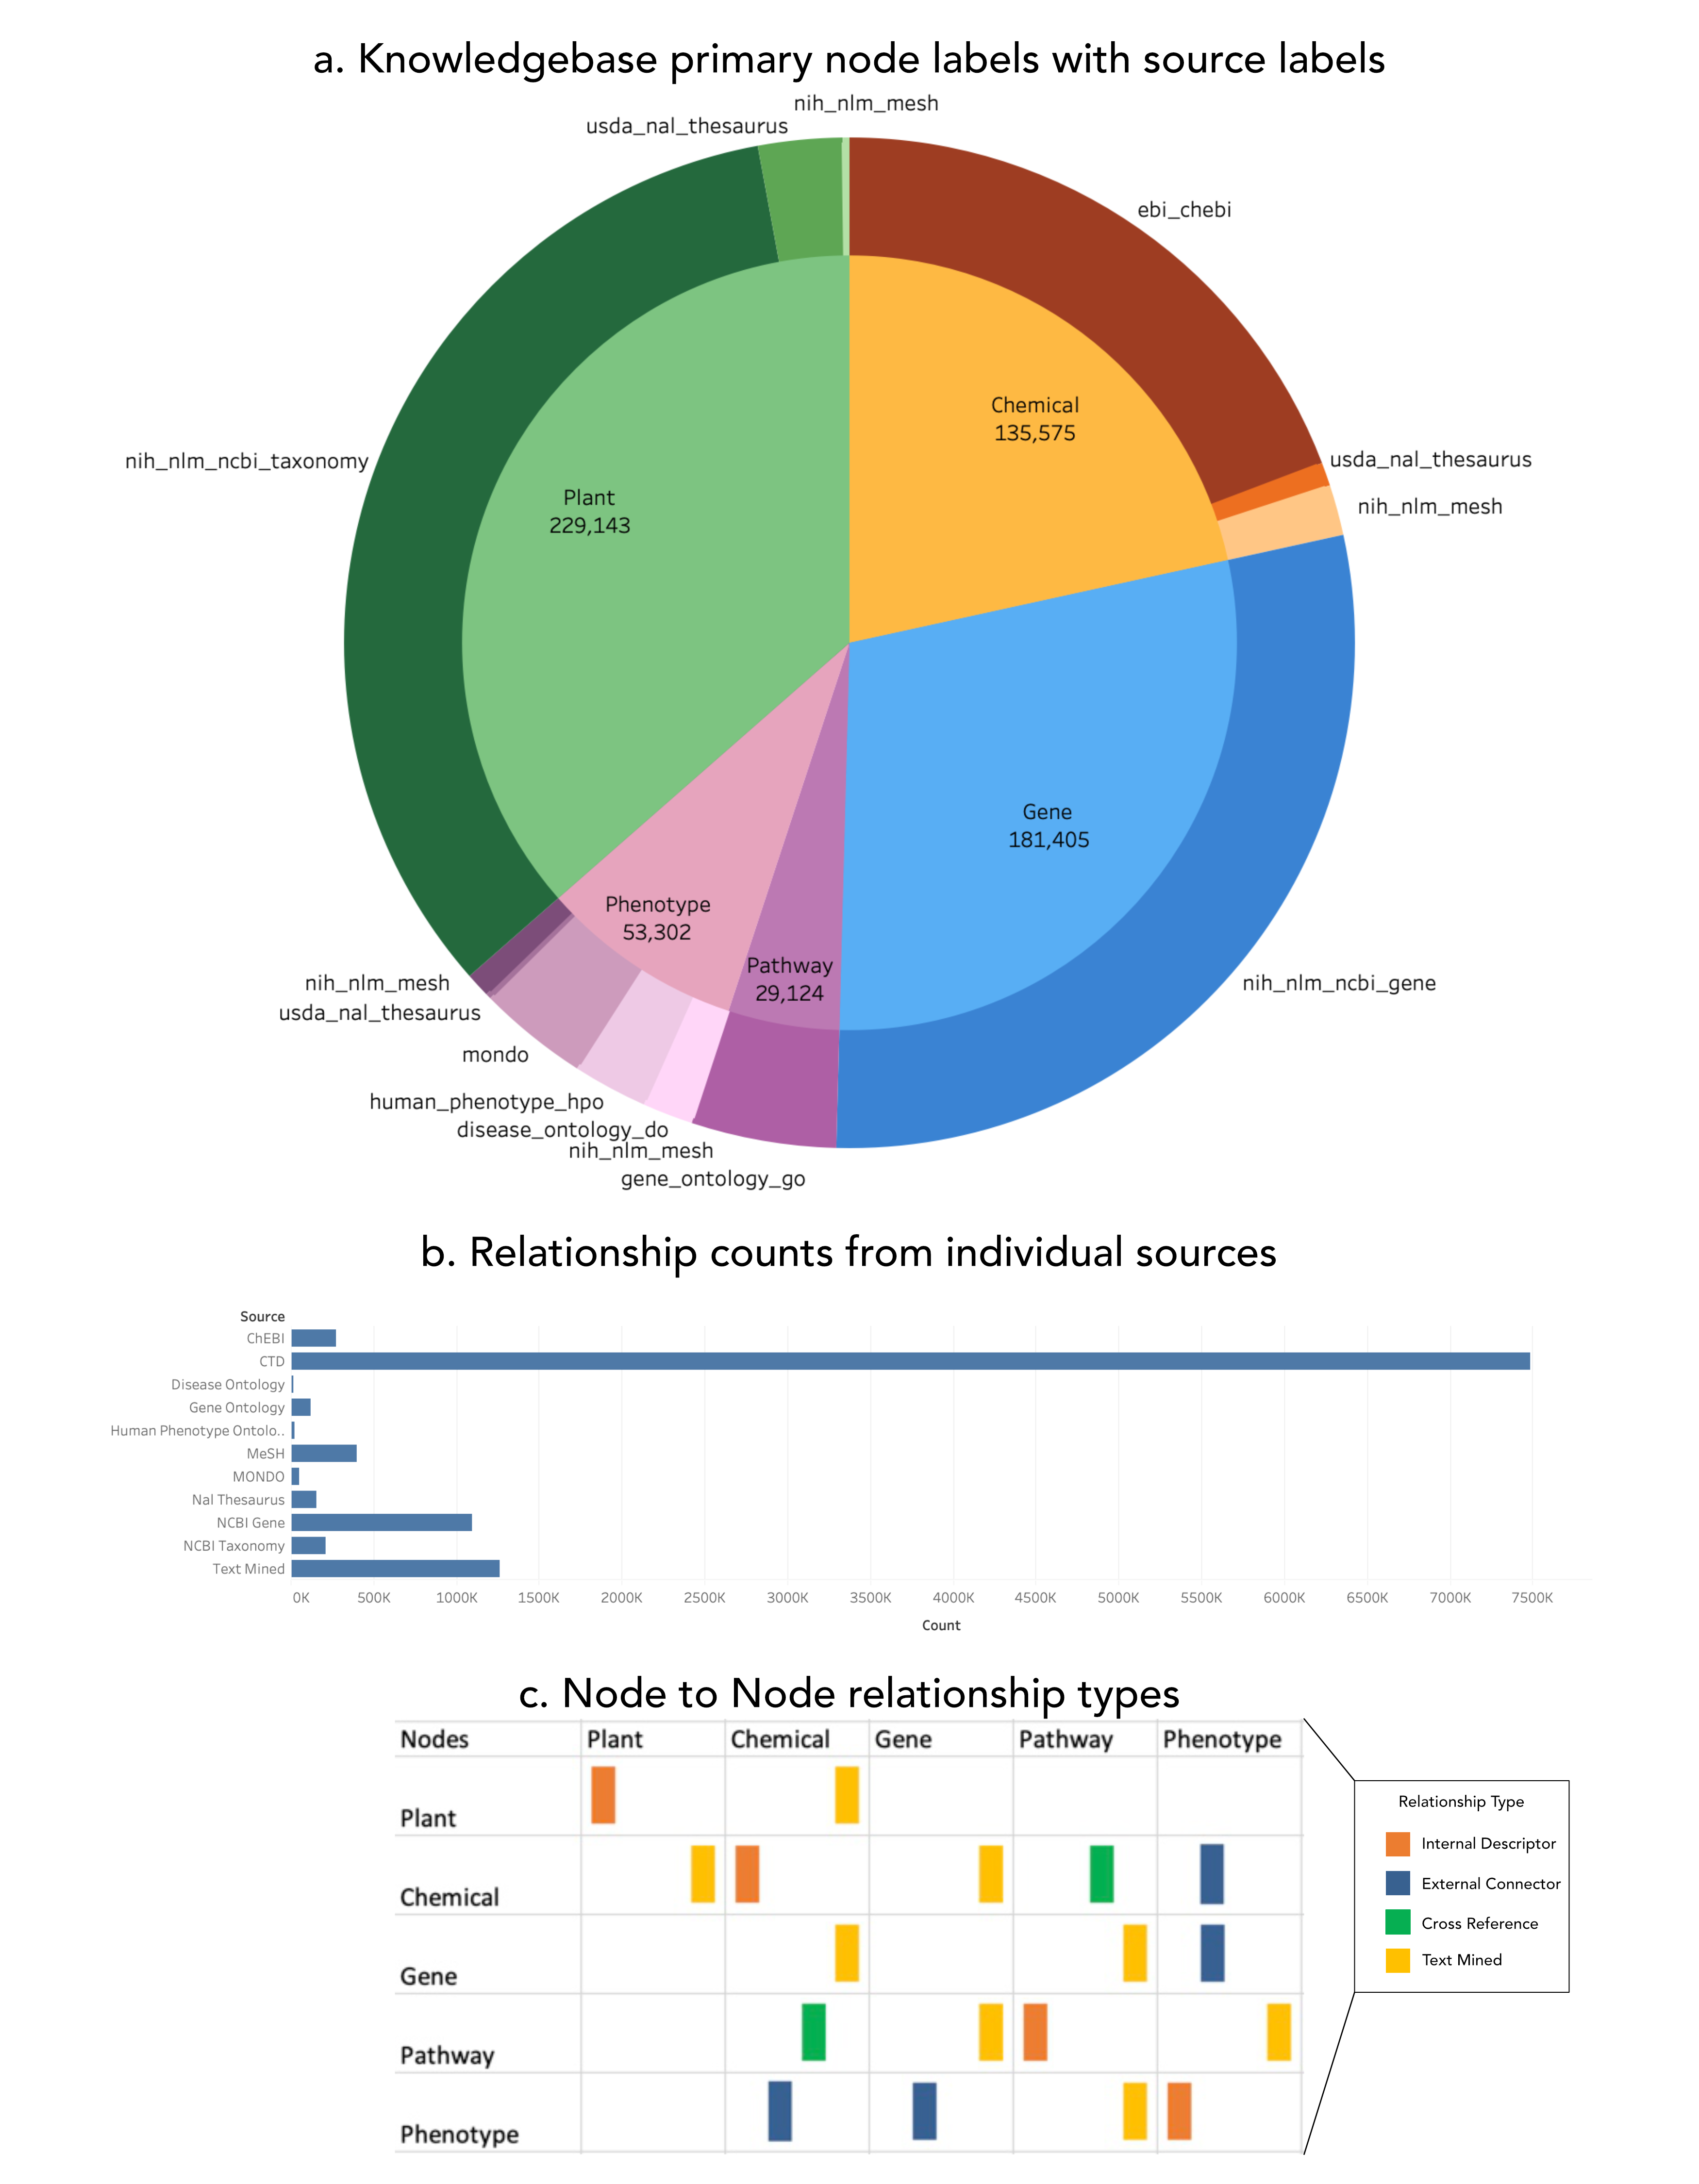
\includegraphics[height=6in]{figs/Fig_2_3.png}
% \par\end{centering}}
% \caption[ABCkb node and relationship statistics]{\label{kb_stats} a. The pie chart shows primary labels indicated by color with named secondary (source) labels, shaded and sized by proportion of total nodes in the knowledgebase. b. The sum of relationship counts for each source is indicated by the bar chart.}
% \end{figure}


% The collection of nodes and relationships in the ABCkb provides novel connections between dietary plants and human phenotypes, and further clarifies connections found in public resources. This is accomplished through the incorporation of molecular associations extracted from literature and structured resources where available. Information in the network flows from plants to phenotypes with assertions in both directions, which allows for query flexibility. Start and end node types are not enforced which allows queries from any point, to any point. To explore the database and discover connections, users have 3 choices: use the provided interface, build graphs with the built in Neo4j interface, or navigate the knowledgebase through a terminal.

% The provided user-friendly interface aids users unfamiliar with Neo4j query language (Cypher) to browse the contents within and examine nutritive connections (Fig.~\ref{kb_interface}). On the home page, users are provided a search box to enter in a search term. This scans the nodes in the knowledgebase and returns results ranked by similarity to search term. Users can select nodes and continue to build a query to any end point within the knowledgebase (plant, chemical, gene, pathway, or phenotype). Running the query scans the database for all paths to the selected end point and returns them to the user, which are available to download. Additionally, a Cypher query is available to users that can be used in the built in Neo4j interface or the terminal.

% \begin{figure}[!h]
% {\begin{centering}
% 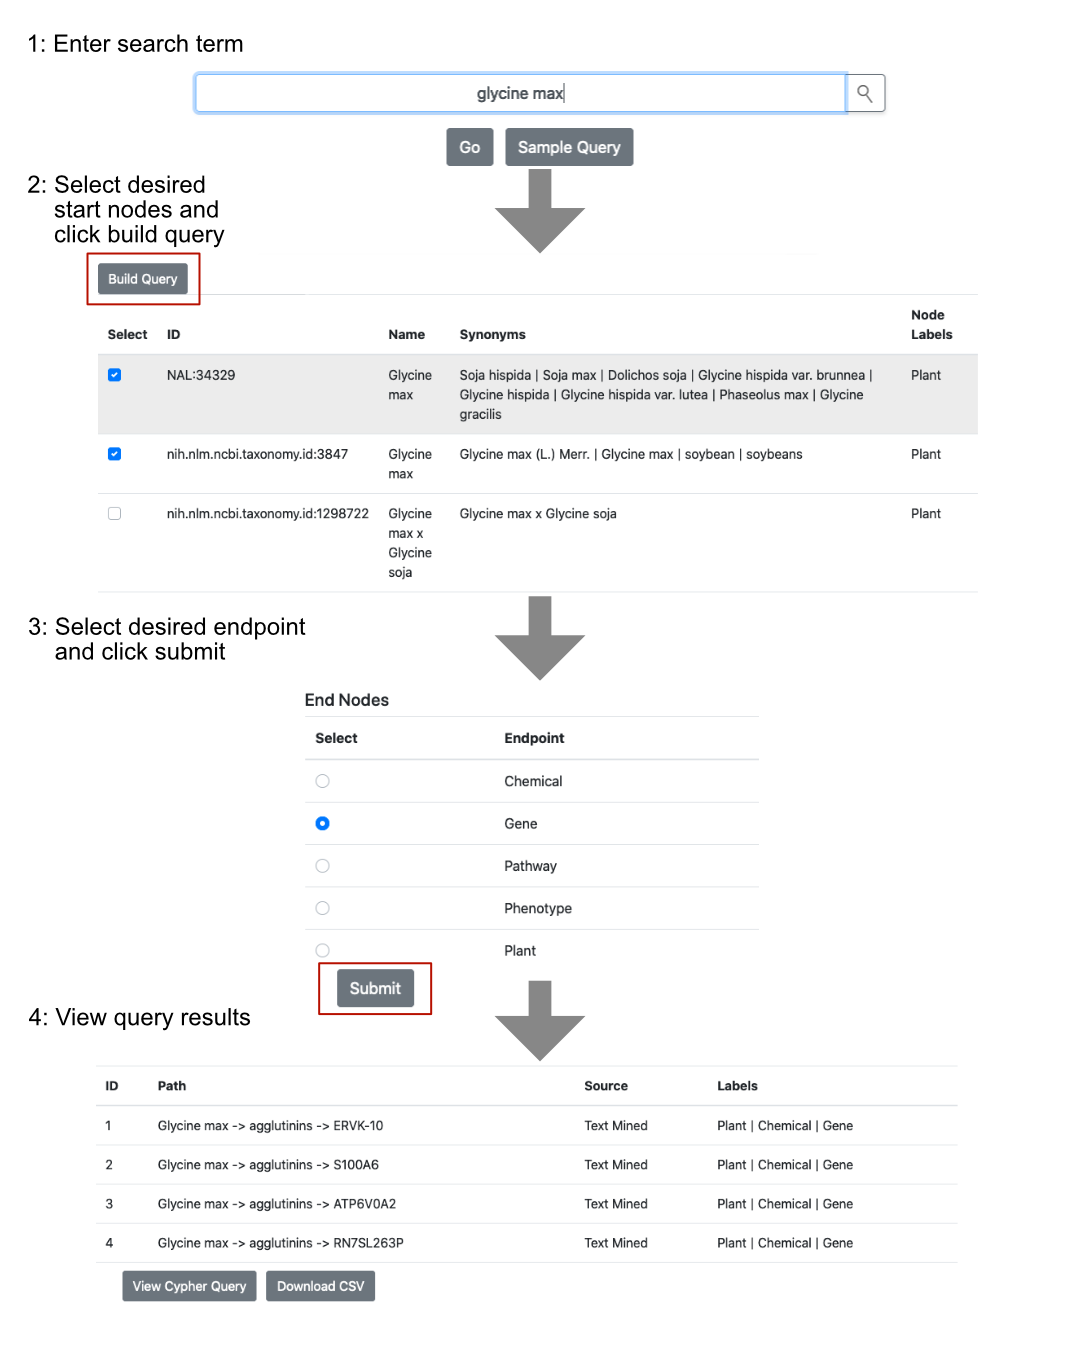
\includegraphics[height=6in]{figs/Fig_2_4.png}
% \par\end{centering}}
% \caption[Browsing the ABCkb Interface]{\label{kb_interface} There are 4 primary steps to browsing using the provided interface. Once the query endpoint is selected and the user clicks submit, they have the option of downloading all results as a csv, or viewing the Cypher query.}
% \end{figure}

% \subsubsection{Oat and T2D}

% To demonstrate how the ABCkb connects dietary plants to separate human indications through molecular mechanisms, a graph was created in the ABCkb depicting the diet-disease network between \textit{Avena sativa}, T2D, and heart failure (Fig~\ref{av_2_diab}). This network indicates that consumption of oats affects cholesterol levels in the body, which in turn is associated with the gene HSD11B1 that affects lipid metabolic processes with both positive and negative impacts on the incidence of T2D. These relationships are due to the presence of beta-glucan in oat grains. Consumption of beta-glucan-containing oat can help lower LDL cholesterol~\cite{wolever_oat_2016}. The cholesterol lowering effects of oat can also be attributed to the presence of certain lipids and proteins~\cite{guo_cholesterol-lowering_2014}. The proteins in oat with low lysine-arginine and methionine-glycine ratios contribute to lower total cholesterol and LDL cholesterol levels. Hypocholesterolemic properties of oat cannot simply be attributed to one factor, but a combination of many, including oleic acid, vitamin E, and plant sterols~\cite{guo_cholesterol-lowering_2014}.

% \begin{figure}[!h]
% {\begin{centering}
% 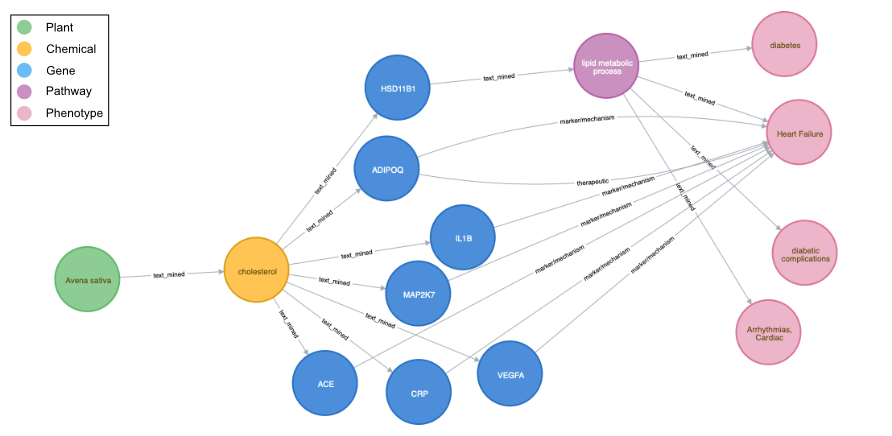
\includegraphics[height=3in]{figs/Fig_2_5.png}
% \par\end{centering}}
% \caption[Visualizing the results of \textit{Avena sativa} to diabetes and heart failure via Hydroxysteroid 11-Beta Dehydrogenase 1.}
% This meta-path highlights the connectivity between oats, diabetes, and heart failure through the gene HSD11B1 from the ABCkb.}

% % Generated with:
% % MATCH p=(:Plant {source_id:"nih.nlm.ncbi.taxonomy.id:4498"})-->
% %        (:Chemical {name:"cholesterol"})-->
% %        (:Gene {name:"HSD11B1"})-->
% %        (:Pathway {source_id:"GO:0006629"})-->
% %        (ph:Phenotype) 
% % WHERE ph.name =~ "diabet.*" OR 
% %         ph.name =~ ".*eart.*" OR 
% %         ph.name =~ ".*ardiac.*"
% % RETURN p
% \end{figure}

% T2D patients frequently have abnormal levels of many different lipids, as well as abnormal qualities to these lipids, for example, T2D patients experience normal or slightly elevated LDL cholesterol with increased LDL oxidation and glycation~\cite{verges_new_2005}. Dyslipidemia in T2D patients is associated with cardiovascular disease ~\cite{pokharel_prevalence_2017,shahwan_prevalence_2019}. This creates an elevated risk for cardiovascular diseases including atherosclerosis, and dislipidemia may play a role in these risks~\cite{shahwan_prevalence_2019}. In the graph, HSD11B1 is the human gene connecting this relationship. HSD11B1 expression is increased in adipose tissues of obese individuals~\cite{paulsen_11beta-hsd_2007}. Dysregulation of HSD11B1 is associated with an imbalance of glucocorticoid in adipose tissues, glucose imbalance, and visceral fat accumulation~\cite{dammann_expression_2019}. These factors contribute to metabolic syndrome, which puts patients at a higher risk for cardiac diseases~\cite{turek_gender-dependent_2014}. Various SNPs in HSD11B1 have associations with T2D, metabolic syndrome, and hypertension~\cite{nair_11beta-hydroxysteroid_2004,gambineri_combination_2011,freedman_distribution_2001,goff_insulin_2005}. 

% Due to the established relationship between oat beta-glucans, cholesterol, and weight, the connection to T2D is logical~\cite{wolever_oat_2016,dammann_expression_2019}. Decreased weight, specifically visceral fat in the abdomen, would result in reduced expression of HSD11B1, which would improve regulation of cortisol. Further examination of the oat - cholesterol - HSD11B1 relationship could be very informative to both patients and doctors in making more informed dietary choices and reducing the risk of developing T2D. This example demonstrates the ABCkb ability to connect seemingly separate conditions through the molecular mechanistic links within.

% \subsection{Discussion}

% The ABCkb integrates structured and unstructured resources in a network that connects plants to human disease through molecular mechanisms. This reduces the time required to manually connect these links through each individual resource. Additionally, knowledge discovery is aided by the development of a user-friendly interface. All of these components provide precision nutrition a path to better understand the mechanisms behind diet-related conditions. The ABCkb is available from github (https://github.com/atrautm1/ABCkb).

% ######

% \section{Updates, Upgrades, and Other Uplifts}

% To highlight gaps in current knowledge, the data within the KB must be current. Scripts to build the KB were originally written in Python 2 which was deprecated at the end of 2019, so we started by converting the scripts to Python 3. All of the scripts were cleaned up and put into modules to yield 4 steps to create the knowledgebase. This will aid in the utility of the KB so that others can build a version locally or add sources to connect. 

% \subsection{Reducing Graph Density}

% Great effort was made in the knowledgebase to model predicates between subjects and objects. This effort resulted in a large degree for each node with some predicates providing non-useful information other than an additional edge between two nodes. The time complexity of traversing any graph is calculated by the formula \(O (V + E) \) where \(V\) is the number of vertices in the graph and \(E\) the number of edges. Currently there are 18.7 million nodes and 446 million edges in the knowledgebase.  The end result for the user of the knowledgebase is a slow tree traversal and graph building as neo4j iterates over each possible path. Consider table \ref{tab:Table1} with graph build times and queries on a high performance research cluster utilizing one terabyte of memory and 1 compute node with 32 processors per node which demonstrates the density of the graph with edges far outnumbering nodes.

% \begin{table}[H]
% \begin{centering}
%     \centering
%     {\small{}}%
%     \begin{tabular}{|c|c|c|c|c|}
%     \hline
%     {\small{}Query} & {\small{}Total Nodes} & {\small{}Total Edges} & {\small{} Density (*100)} & {\small{} Time (s)}\tabularnewline
%     \hline
%     \hline
%     {\small{}A} & {\small{}1,228} & {\small{}3,615} & {\small{}0.24} & {\small{}5.1}\tabularnewline
%     \hline
%     {\small{}B} & {\small{}7,869} & {\small{}82,363} & {\small{}0.13} & {\small{}7.4}\tabularnewline
%     \hline
%     {\small{}C} & {\small{}18,373} & {\small{}277,278} & {\small{}0.082} & {\small{}168.9}\tabularnewline
%     \hline
%     {\small{}D} & {\small{}-} & {\small{}-} & {\small{}-} & {\small{}>86,400}\tabularnewline
%     \hline
%     \end{tabular}
    
% \par\end{centering}{\small \par}
% \caption[Original KB: Build times with Node and Edge counts.]{\label{tab:Table1}Build times for traversing the graph with graph density from \textit{Glycine max} to Chemicals (A), to Genes (B), to Pathways (C), and to Phenotypes (D) in the old database }
    
% \end{table}

% To reduce graph density, parallel text-mined edges between two nodes were collapsed into a singular edge. Predicates are also stemmed using the Snowball stemming algorithm to reduce the size of the information contained within each edge. Table \ref{tab:Table2} shows the effects of the improvements on graph density.


% \begin{table}[H]
% \begin{centering}
%     \centering
%     {\small{}}%
%     \begin{tabular}{|c|c|c|c|c|}
%     \hline
%     {\small{}Query} & {\small{}Total Nodes} & {\small{}Total Edges} & {\small{} Density (*100)} & {\small{} Time (s)}\tabularnewline
%     \hline
%     \hline
%     {\small{}A} & {\small{}1,600} & {\small{}1,599} & {\small{}0.063} & {\small{}3.8}\tabularnewline
%     \hline
%     {\small{}B} & {\small{}21,196} & {\small{}233,354} & {\small{}0.052} & {\small{}11.6}\tabularnewline
%     \hline
%     {\small{}C} & {\small{}31,024} & {\small{}438,739} & {\small{}0.046} & {\small{}116}\tabularnewline
%     \hline
%     {\small{}D} & {\small{}9,000} & {\small{}167,941} & {\small{}0.21} & {\small{}151}\tabularnewline
%     \hline
%     \end{tabular}
    
% \par\end{centering}{\small \par}
% \caption[Updated KB: Build times with Node and Edge counts.]{\label{tab:Table2}Updated KB build times for traversing the graph with graph density from \textit{Glycine max} to Chemicals (A), to Genes (B), to Pathways (C), and to Phenotypes (D) }
    
% \end{table}

% \subsection{Updating source data}
% Sources contained within the knowledgebase and used for text-mining have been updated with current data. The indexes for MEDLINE and AGRICOLA were updated with abstracts from May, 2019. The former Linguamatics NLP queries were rerun using updated ontologies and indexes and added to the knowledgebase. The effects of the updated information can be seen in table \ref{tab:Table3}. This will build a substantial foundation for the microbiome data to link to, and provide researchers with up-to-date information for hypothesis generation. 

% \begin{table}[H]
% \begin{centering}
%     \centering
%     {\small{}}%
%     \begin{tabular}{|c|c|c|}
%     \hline
%     {\small{}Label} & {\small{}Old DB} & {\small{}New DB} \tabularnewline
%     \hline
%     \hline
%     {\small{}Plant} & {\small{}170,656} & {\small{}208,345} \tabularnewline
%     \hline
%     {\small{}Chemical} & {\small{}116,768} & {\small{}121,214} \tabularnewline
%     \hline
%     {\small{}Gene} & {\small{}16,695,943} & {\small{}199,183} \tabularnewline
%     \hline
%     {\small{}Pathway} & {\small{}30,486} & {\small{}29,457}\tabularnewline
%     \hline
%     {\small{}Phenotype} & {\small{}11,801} & {\small{}27,154}\tabularnewline
%     \hline
%     {\small{}Bacteria} & {\small{}0} & {\small{}497,523}\tabularnewline
%     \hline
%     {\small{}Total} & {\small{}17,025,654} & {\small{}1,082,876}\tabularnewline
%     \hline
%     \end{tabular}
    
% \par\end{centering}{\small \par}
% \caption[Comparing original and updated KB contents. ]{\label{tab:Table3}Updated KB node counts compared to the old KB. }
    
% \end{table}

% \section{Download Full Text Articles}

% Though abstracts remain popular for text mining due to ease of use and availability, previous work has revealed that they do not contain all important findings from papers, and mining through full text articles reveals more hidden associations\cite{westergaard_text_2017}. There are two challenges with this method, downloading and indexing full text articles and reducing artificial noise 

% \subsection{Identify Target Papers}

% To identify which papers to download, the MEDLINE and AGRICOLA indexes previously used to generate the KB were mined to find instances of gut microbiome with mouse or human and a subset of 26 bacterial families common to the human gut microbiome\cite{qin_human_2010}. We limited the results to exclude review papers and papers which may inflate database query results and create difficulty with generating hypotheses. This method yielded over 35,000 articles for downloading and indexing. 

% \subsection{Development of An Automated Paper Scraper}

% Downloading full text articles has two main parts, obtaining permission for text and data mining with each publisher, and downloading articles. After obtaining permission from each respective publisher, we were left with a subset of about 28,000 articles. An automated paper scraper, aptly titled PaperScraper, was developed to programmatically download articles. It takes input Digital Object Identifier (DOI) information, checks it against a database, Crossref, and outputs an article in a form that the user selects (PDF, XML, or HTML) In addition, the PubMed Central (PMC) open access papers can be scanned and downloaded. This module was coded in Python 3, and should be used with care and communication with an institution's respective library, as many have Terms and Conditions not publicly published which may limit programmatic access of journal content. This subset of articles was indexed in Linguamatics to be used for text mining.

% \section{Text mining}

% Relationships will be mined out as triples for use in the KB. This process will require various ontologies to properly categorize extracted elements. An ontology is a set of hierarchichally grouped data, sometimes called classes, which can be used to convey relatedness, properties of classes, and organized in logical orders. A bioinformatic counterpart to ontologies are phylogenetic trees which are often organized in a similar fashion. Linguamatics indexes articles using specified ontologies for developing NLP queries. NLP will be used to answer the questions of how bacteria are affected by chemicals, how bacteria metabolize and affect chemicals, how bacteria are affected by and affect diseases and phenotypes, and how specific diets influence bacterial abundances.

% \subsection{Reduce Artificial Noise}

% A challenge of using full text is reducing artificial noise. This is especially seen in PDFs converted to text for indexing. A subset of 62 articles in PDF format have been manually annotated with bacterial information for the development of an NLP query that limits false positive matches. This will bolster the accuracy of the query and the resulting KB.

% \section{Load into the KB}

% The text mining query results will be loaded into a neo4j graph database containing data linking plants to human health. Python 3 scripts will be developed to facilitate the process for loading the data into neo4j. The data will be converted from the output tab separated format into a format that neo4j will accept and import. Similar to the rest of the KB, predicates will be stemmed and parallel text-mined edges will be collapsed. The predicates will be added as a property of each edge in array form which will increase query speeds improving the utility of the knowledgebase. 


\chapter{ADDITION OF MICROBIOTA DATA TO ABCKB FROM FULL TEXT LITERATURE}

% Outline

% Intro pgrph

% History of Microbiota/Microbiome research
%   - The way things used to be
%   - Where we are now
%   - Why the need for a knowledgebase
% Structured data sources
%   - Disbiome
%   - NCBI Taxonomy
%   - 
% Unstructured data sources
%   - Difference between using abstracts and full text
% Methods
%   - New ABCkb schema
%   - Searching for full text articles
%   - Extracting full text articles
%   - Mining full text articles
%   - Addition to the knowledgebase


Modeling diet to disease includes more than the phytochemicals from plants and the human genes they affect upon ingestion. A community of micro-organisms exists within the digestive system of humans that maintains a symbiotic relationship, though not always beneficial for the host. Two primary diseases associated with this community, Irritable Bowel Syndrome (IBS) and Inflammatory Bowel Disease (IBD), are both increasing in prevalence and diet related \cite{abdul_rani_irritable_2016}. The term microbiota refers to the collection of bacterial species within the gut, where the microbiome refers to the collective genomic data present in the gut \cite{ursell_defining_2012}. Specific microbiota have been implicated in various digestive disorders, and the impact of microbiota on diet and compounds descending the alimentary canal has been a topic of recent interest.

\section{History of Microbiome Research}

Historically, an abiotic existence was argued for by the majority of biologists as microbiota were thought to be solely drivers of diseases. This thought prevailed through the 1950's until researchers discovered bacteria present within healthy mice grown in sterile conditions \cite{prescott_history_2017}. This, along with improvements in sequencing technologies, allowed for the identification of bacteria present within the human gut and the discovery that these bacteria exist in communities \cite{ursell_defining_2012}. The shift in health research to include microbiota resulted in the human microbiome project that set out to elucidate the single microbiota formulation for optimal human health \cite{turnbaugh_human_2007}. Controversially, no one, single formulation is found to be the best but rather a conglomeration of abundances provides protective benefits to the host. Increased abundances of opportunistic bacteria result in digestive disorders due to the fermentation of sugars within the gut and promotion of inflammatory molecules \cite{wallen_characterizing_2020}. The goal of microbiome research is to maximize the abundances of good bacteria, or probiotics. The levels of bacteria are largely attributed to dietary components and compounds, called prebiotics. 

\subsection{Probiotics}

Probiotics have risen in popularity in the 21st century. The widely accepted definition of probiotics from the WHO is that they are "live strains of strictly selected microorganisms which, when administered in adequate amounts, confer a health benefit on the host" \cite{mack_probiotics_2005}. Often probiotic strains are specifically developed for use in commercial products like supplements, fermented beverages, or yoghurts. 

\subsection{Prebiotics and diet}

Prebiotic compounds encourage the growth of probiotic bacteria and are generally fermented by probiotic bacteria. Common examples of prebiotics are inulin, resistant starches, and dietary fibers \cite{davani-davari_prebiotics_2019}. These prebiotic compounds can be found in supplements, or via natural sources. Complications arise in patients with IBS and IBD that are advised to follow a low FODMaP (Fermentable Oligo, Di, Mono and Polysaccharide) diet, which reduces digestive symptoms along with probiotic bacteria \cite{halmos_diets_2015}. As prebiotics impact probiotic abundances, so also does diet as a whole. Many studies have found that microbiota communities are largely affected by diet, stronger than genetic drivers often seen segregating by geographic regions \cite{singh_influence_2017,goertz_geographical_2019,gupta_geography_2017}. This is likely due to the availability of various foods in regions and cultural differences. However regional cultural or otherwise defined, diet is largely constructed of chemical components whether naturally derived or synthetically produced.

Therefore, we set out to provide a knowledgebase through which the effects of diet on human health could be examined in conjunction with the various interactions between specific bacterial taxa within the gut, and the phytochemicals contained in plant compounds.

\section{Structured Data Sources}

Few resources are available on the interaction between microbiota and human health. Mentioned previously, the Human Microbiome Project provides raw data to researchers, which can be used to compare to raw data from experimental conditions, or reanalyzed to drive new insights\cite{turnbaugh_human_2007}. However, no associations are provided in a human readable format. Recently developed, the Disbiome database provides a queriable resource to catalogue the interaction between microbiota and disease \cite{janssens_disbiome_2018}. No molecular mechanisms are provided with Disbiome. There are no databases that provide microbiota to diet, or dietary compounds, currently available. The NCBI Taxonomy will provide bacteria nodes which will be used in NLP queries to generate links between microbiota, diet, and human health.

\section{Unstructured Data Sources}

The majority of microbiota interactions are not held within structured data sources, but rather in published, unstructured research. Therefore, a method is necessary to extract and place those assertions into the ABCkb. Previously, we used I2E to extract assertions for every step in the pathway from MEDLINE abstracts. Recent research has highlighted the need to develop methods that can extract assertions from full text, as additional assertions are not contained within the abstract \cite{westergaard_text_2017,westergaard_comprehensive_2018}. The addition of microbiota data to the knowledgebase is a key component to determine how diet affects human health and move towards a personalized solution to nutrition.

\section{ABCkb 2.0 Methods}

Using the ABCkb as a starting point, the microbiome information integrates with the existing knowledgebase (Figure ~\ref{Fig_3_1}). The visualized schema shows the bi-directionality of the microbiota on plant compounds, along with general assertions provided from the ABCkb 1.0 linking diet and disease. The logic is simple. Often, links in literature are provided, much like the disbiome resource, where a bacteria is linked with a disease. These links are generated through association studies and molecular mechanisms are simply unknown. The ABCkb 2.0 will provide both the general links (from bacteria to disease) and possible molecular mechanisms for those diseases (from genes to disease). Researchers will be able to use this knowledgebase to generate testable hypotheses about the unknown from what is known. However, unlike the first iteration of the ABCkb, we will be extracting microbiome assertions from full text articles.  

\subsection{Identifying Relevant Full-Text Articles}

To identify a suitable subset of full-text articles for text mining, a query was developed that locates instances in PUBMED abstracts of microbiome, with related synonyms from MeSH, NAL Thesaurus, and NCBI Taxonomy, and one of either \textit{Homo sapiens}, \textit{Ratticus norvegicus}, and \textit{Mus musculus} with their respective synonyms. The sources that provided these matches with synonyms were the NAL Thesaurus, MeSH, and the NCBI Taxonomy database. These three hosts were chosen for their relevance to human health and to remove any non-related biological hosts. This query identified over 30,000 unique articles for full-text extraction from abstracts in MEDLINE in May, 2019.

\subsection{Extracting Full-Text Articles}

Full text articles were extracted first through obtaining permission from the publishers. This process took approximately 6 months to complete. Permissions to extract and mine through 23,000 of the original 30,000 was acquired with the assistance of the UNC Charlotte Library from current and updated license agreements. An automated paper scraper was developed to pull pdf, xml, and txt files from PUBMED article identifiers. This tool is available from GitHub as a standalone resource.

\subsection{Text Mining Full-Text Articles}
Extracting assertions from articles was performed with two primary functions, entity recognition and relationship extraction. Entity recognition is the function of recognizing specific entities (Plant, Chemical, Gene, Pathway, Phenotype, Bacteria, Diet), which yield start and end nodes in the knowledgebase. I2E employs a user-specified dictionary based approach to entity recognition. We utilized a set of ontologies and structured vocabularies for this process (Figure ~\ref{er_sources_abckb2}). Each of these sources were used in I2E queries to extract the 7 entity types (nodes) provided in the knowledgebase.

\begin{figure}[!h]
{\begin{centering}
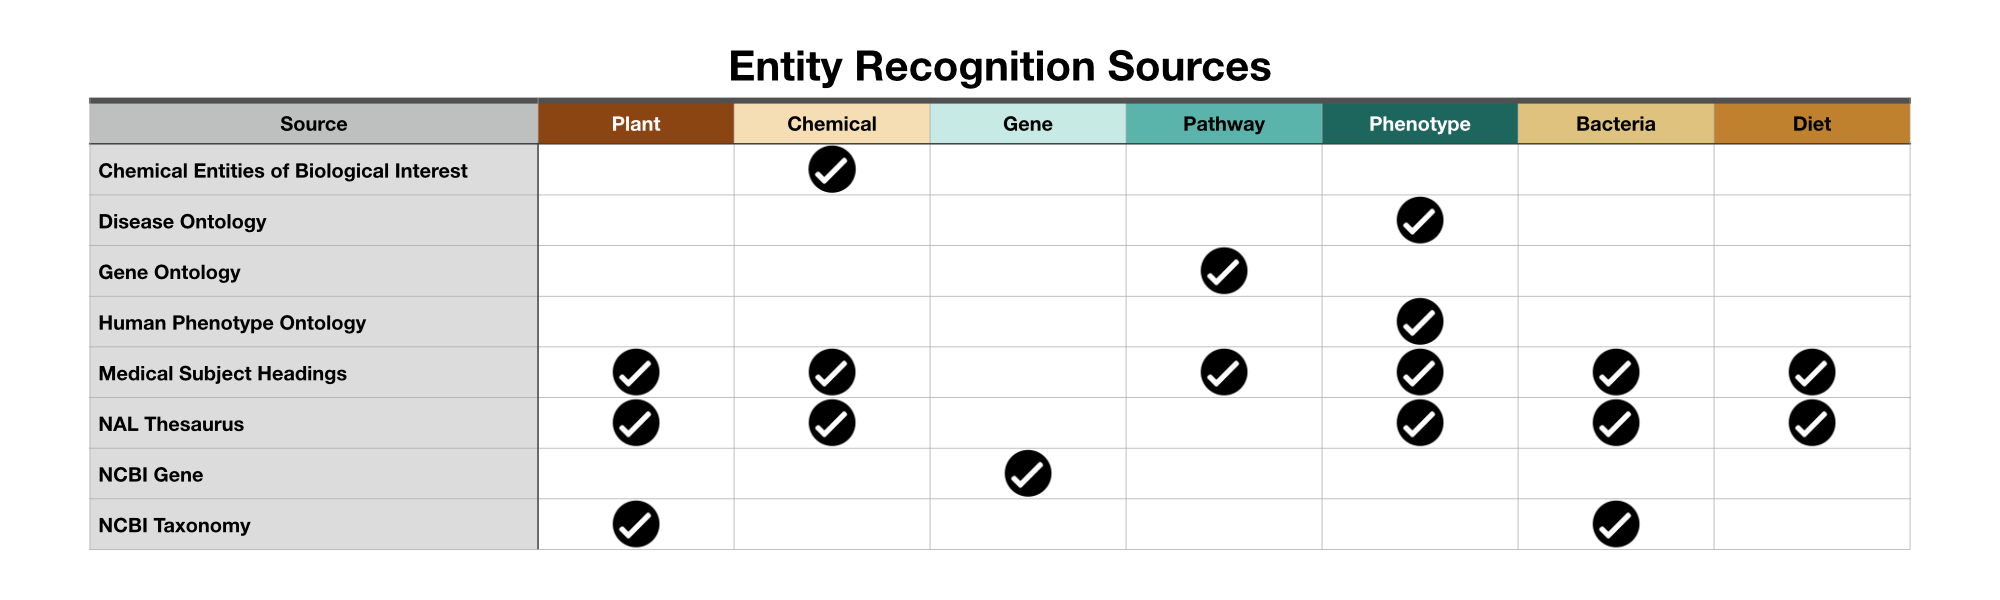
\includegraphics[width=6in]{figs/Entity_Recognition_Sources.png}
\par\end{centering}}
\caption[ABCkb 2.0 Entity Recognition Sources]{\label{er_sources_abckb2} There are a total of 8 sources used for entity recognition in I2E. These 8 sources provide all of the nodes in the Knowledgebase as indicated in the figure.}
\end{figure}

Bacterium in literature are often abbreviated for brevity which is a hurdle for dictionary based text mining tools to overcome given the dictionary, in many cases, does not contain the abbreviation. This is a result of multiple genera sharing the same species name, in some cases an indication of function (\textit{Halolactibacillus halophilus} and \textit{Halobacillus halophilus}). 

The abbreviated bacterium identification hurdle was overcome by using, a combined process of text mining with the rule/dictionary method in I2E to identify all mentioned bacterium in the article, and a separate regular expressions query to identify abbreviated matches. Each abbreviated match in a single article is compared to the set of bacterium mentioned for each article to map back to the original node identifier and thus extract the specific bacterium for each relationship. The additional specific entities were well-defined within the structured vocabularies used for text-mining and did not require additional mappings.

Once the entities were categorized, relationship extraction was the next step. I2E by Linguamatics provided 21 sentence models for extracting assertions, however, a specified predicate ontology was used and iteratively refined to remove false positive results. Text-mining through full-text articles inherently adds noise through additional text brought in and methods were employed to combat this. Reference matches, though desirable in specific text-mining cases, were not immediately useful to the goal of developing this knowledgebase, and a query was developed to negate matches within the references section. 

The microbiome queries were developed through an iterative process both for entity recognition and relationship extraction (Figure ~\ref{query_ref_fig}). In the summer of 2018, we manually categorized 100 assertions for validation of I2E queries. I2E queries were run against the MEDLINE index and the full-text index and judged by measures of precision and accuracy. Manually we refined the queries until reaching a F-score threshold of 85\% for entity recognition and F2-score threshold of 85\%. The F2 score was chosen for a higher recall rate over precision given our focus of hypothesis generation, to maximize possible connections between entities.

\begin{figure}[!h]
{\begin{centering}
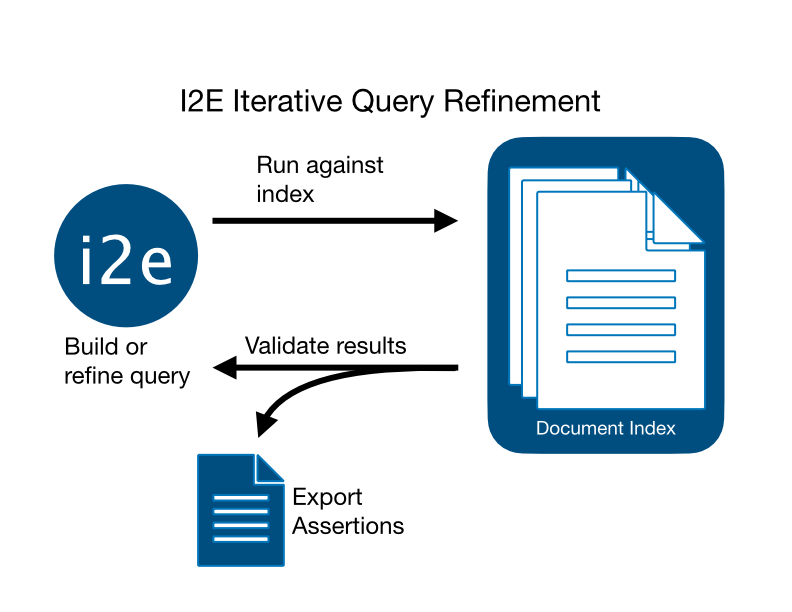
\includegraphics[width=6in]{figs/Iterative_Query_Refinement.png}
\par\end{centering}}
\caption[I2E Query Development]{\label{query_ref_fig} Iteratively developing I2E queries is a process of 1. Building a query, 2. Running the query against the document index, and 3. Validating the results returning either to refine the query or export the results when reaching a satisfactory threshold.}
\end{figure}

\subsection{Building the ABCkb 2.0}

After extracting Nodes and relationships from public sources, node and relationship reduction steps were necessary. Duplicate nodes were limited by ensuring node identifiers appeared only once, and collapsing nodes with matching names. To ensure unique nodes present, all node id's from all sources were compared to determine nodes were not defined multiple times. Nodes were further reduced by iterating through the types (Plant, Chemical, Gene, Pathway, Bacteria, Phenotype, Diet) and linking identifiers of a type with the same name into a new identifier. These new node ids are set up by combining "abckb-" with node type (e.g plant, chemical) and an auto-incrementing id. All original source identifiers are retained as a property of the new node along with name and synonyms converted to lowercase for convenience. Relationships originally matched to these original source ids were then remapped to the new knowledgebase ids. All of these extracted, collapsed relationships from full-text and the structured data sources were inserted into the knowledgebase to create the ABCkb 2.0 (Figure ~\ref{Fig_3_1}). This tool will aid researchers to elucidate the molecular mechanisms driving the health effects of the microbiome and diet.

\begin{figure}[!h]
{\begin{centering}
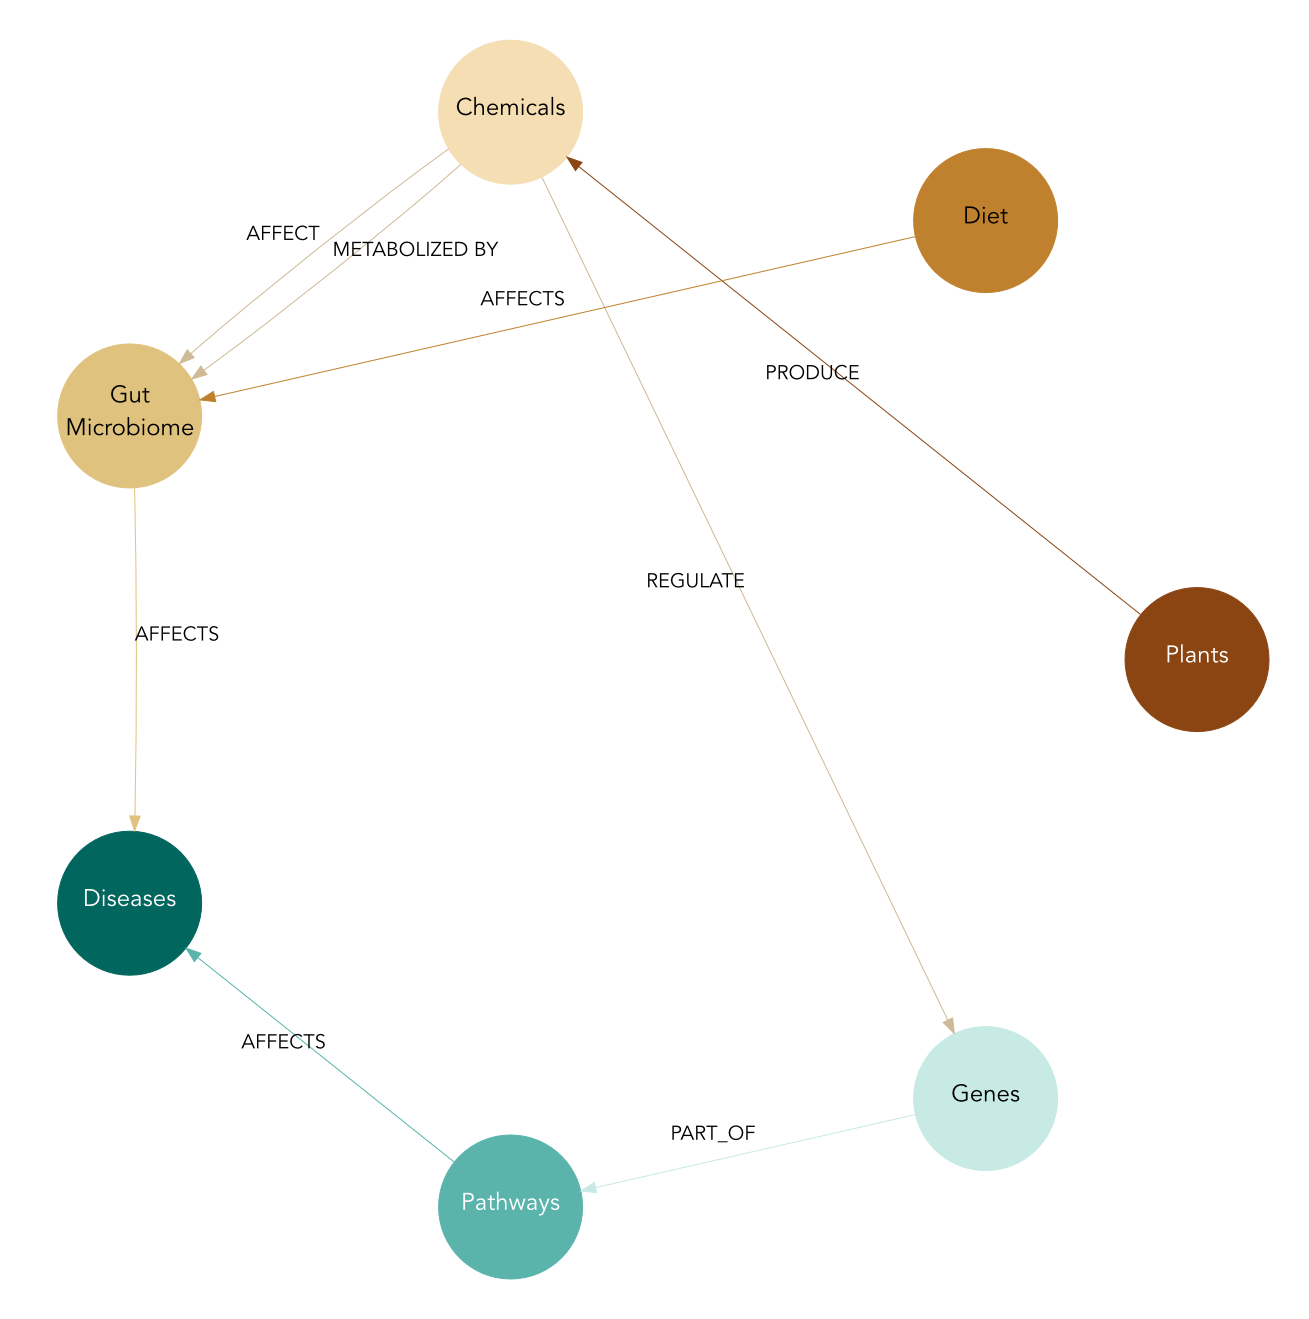
\includegraphics[height=6in]{figs/Fig_3_1.png}
\par\end{centering}}
\caption[ABCkb 2.0 schema]{\label{Fig_3_1} The schema for the ABCkb 2.0 showing connectivity between the additional microbiome portions and the ABCkb 1.0}
\end{figure}

\section{Statistics and Browser}

The ABCkb 2.0 contains 1,155,603 nodes and 7,338,259 relationships, a 60 percent decrease in edges from the first version (table ~\ref{tab:newKBstats}). This is due to the reduction of similar nodes. Full text, text-mining yielded 625,975 hits, which produced 69,206 edges. Over 24,000 novel relationships were found solely in full-text articles and not found in abstracts.  This indicates that mining through the full text increased the amount of associations by a factor of 35 percent. 

\begin{table}[H]
\begin{centering}
    \centering
    {\small{}}%
    \begin{tabular}{|c|c|c|}
    \hline
    {\small{}Node Type} & {\small{}ABCkb v1.0} & {\small{}ABCkb v2.0}\tabularnewline
    \hline
    \hline
    {\small{}Plant} & {\small{}237,350} & {\small{}222,087}\tabularnewline
    \hline
    {\small{}Chemical} & {\small{}156,297} & {\small{}151,336}\tabularnewline
    \hline
    {\small{}Gene} & {\small{}180,669} & {\small{}192,076}\tabularnewline
    \hline
    {\small{}Pathway} & {\small{}28,654} & {\small{}28,759}\tabularnewline
    \hline
    {\small{}Phenotype} & {\small{}54,769} & {\small{}43,428}\tabularnewline
    \hline
    {\small{}Bacteria} & {\small{}0} & {\small{}517,888}\tabularnewline
    \hline
    {\small{}Diet} & {\small{}0} & {\small{}29}\tabularnewline
    \hline
    
    \end{tabular}
    
\par\end{centering}{\small \par}
\caption[ABCkb 2.0 status VS ABCkb 1.0]{\label{tab:newKBstats} The statistics showing the breakdown of node types between the two knowledgebase versions.}
    
\end{table}

The interface browser was updated to include the most recent version of the knowledgebase as a separate browsable data source. Open-discovery queries are the only available query type from the interface. The process begins with the user, entering in a search term in the browser search-bar. This search bar queries a full-text index in Neo4j on node names and node terms, or synonyms. This query produces tabulated results, ranked on search term relevance and limited to the top 10 results to increase efficiency. The user is able to select as many start points as desired and is prompted to click through to the next page. After making selections, the user is prompted to select an endpoint node type (Plant, Chemical, Gene, Bacteria, Pathway, Phenotype, or Diet) where a query is run on pre-assembled paths from the initial node type. This returns all of the possible paths in a table, the ability to download the results to a csv file, and a query that can be used to generate those results in their own neo4j interface.


\section{Application}

\subsection{Phytochemicals, microbiota, and phenotypes}

Phytochemicals have long been touted as semi-magic pills for all kinds of maladies, cancers, and diet-related diseases \cite{khan_comprehensive_2019,guan_review_2021}. For example, plants in the \textit{Brassica} family (broccoli, mustard, and brussels sprouts) contain glucosinolates, a type of phytochemical linked with anti-cancer, antioxidant, and anti-inflammatory benefits (Figure \ref{alistipes}) \cite{verkerk_glucosinolates_2009}. However, there are aspects of this benefit that remain unknown, namely the molecular mechanisms \cite{mazumder_sinigrin_2016}. In the ABCkb (Figure ~\ref{Fig_glu_to_c450}), several genes are linked with glucosinolates, one of which is the cytochrome p-450 gene, CYP4F3 \cite{vang_biochemical_2001}. This gene is one of three key branch points in the arachidonic acid metabolism pathway \cite{wang_metabolism_2021}. Arachidonic acid is released due to stress, injury, and is also found from dietary sources like red-meat, fish, eggs, and poultry \cite{higgins_acute_1984,tallima_arachidonic_2017}. The cytochrome p-450 mediated arachidonic acid pathway has been shown to produce cardioprotective epoxyeicosatrienoic acids\cite{wang_metabolism_2021}. Thus, consumption of glucosinolate-rich foods to influence the breakdown of arachidonic acid through the cytochrome p-450 pathway is of great nutritive importance.

\begin{sidewaysfigure}[!h]
{\begin{centering}
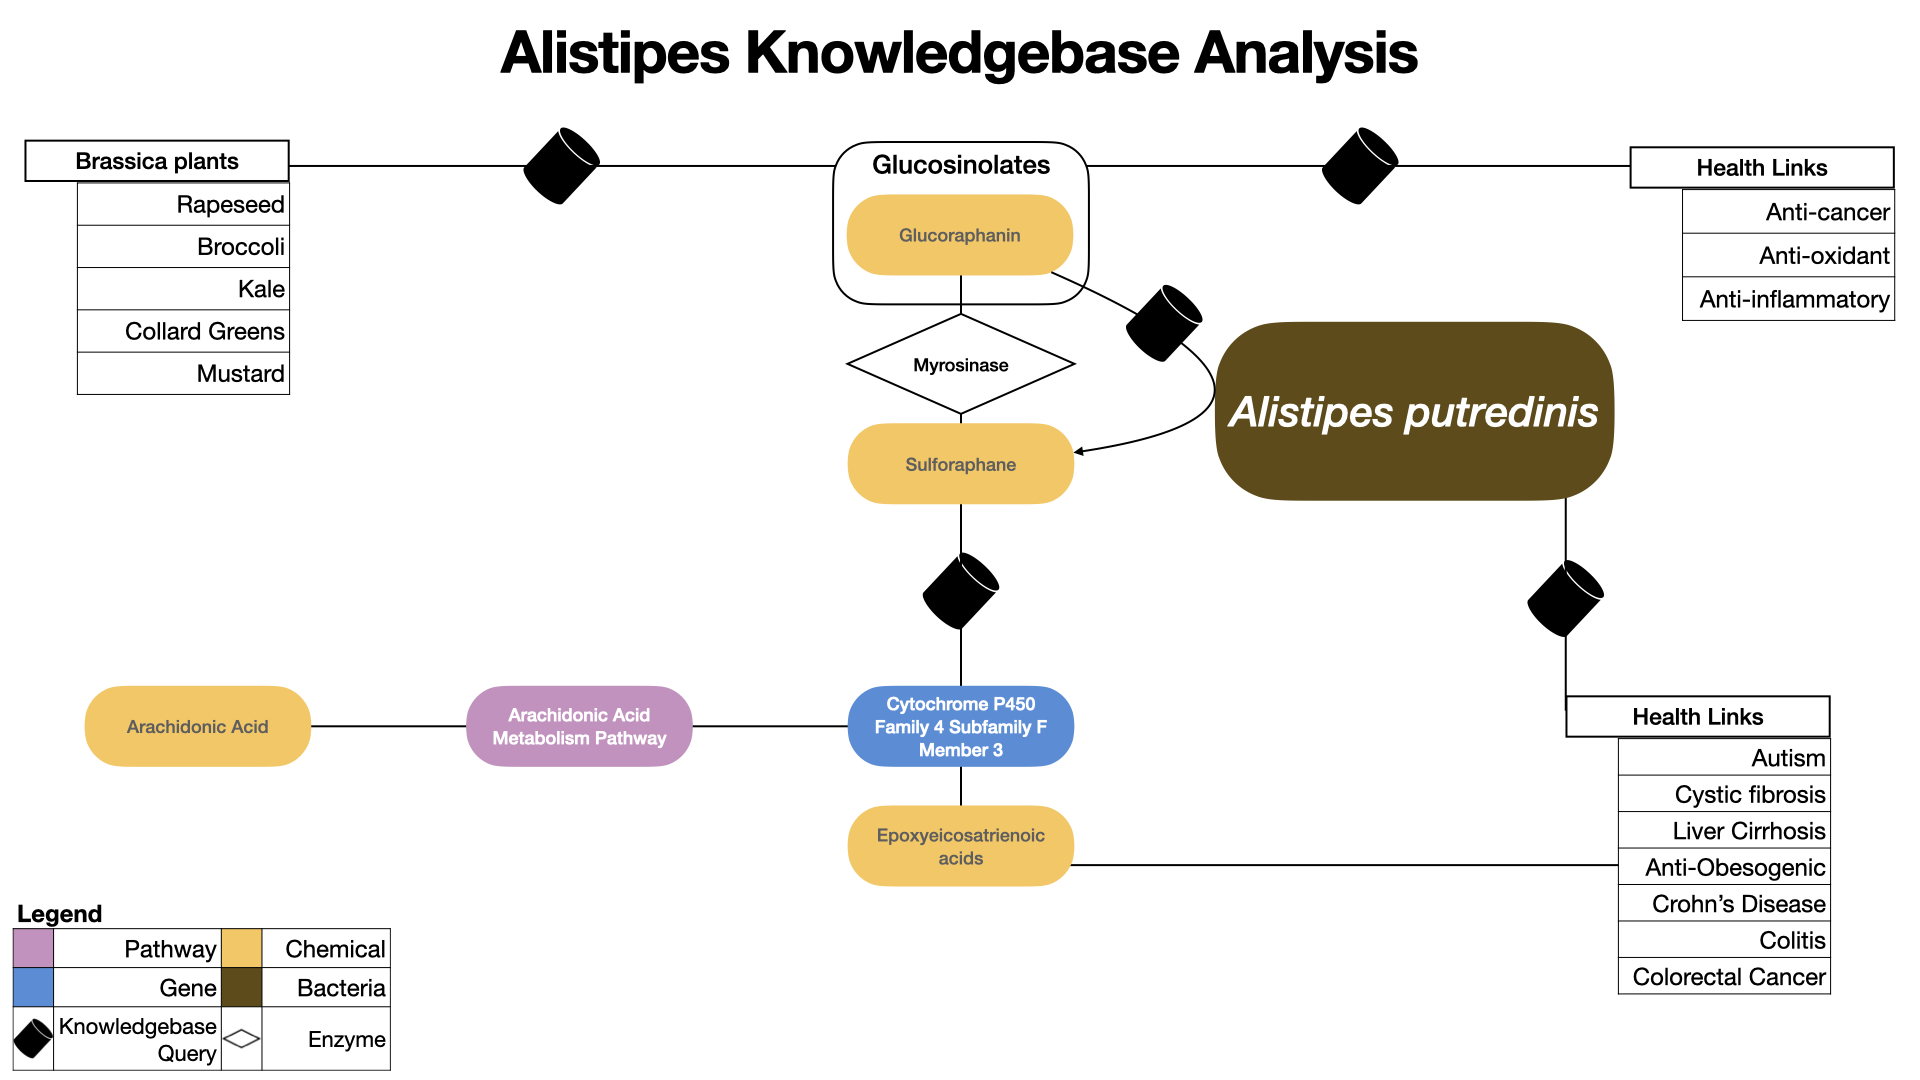
\includegraphics[height=5in]{figs/alistipes.png}
\par\end{centering}}
\caption[Alistipes knowledgebase overview]{\label{alistipes} The overview of the knowledgebase analysis explaining the connection between \textit{Akkermansia spp.}, broccoli, and the claimed health benefits of glucosinolates}
\end{sidewaysfigure}

\begin{figure}[!h]
{\begin{centering}
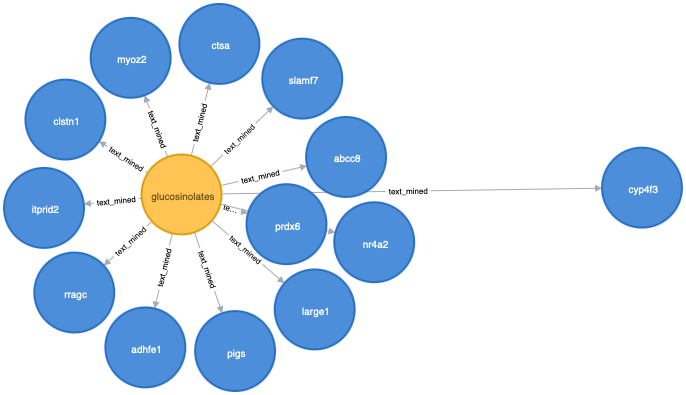
\includegraphics[width=6in]{figs/glucosinolates_to_cyp4f3.png}
\par\end{centering}}
\caption[Glucosinolates to Genes]{\label{Fig_glu_to_c450} A graph from the ABCkb 2.0 showing the connectivity from glucosinolates to genes. One gene in particular has been singled out, Cytochrome p-450.}
\end{figure}

However, glucosinolates like glucoraphanin are not activated unless they are transformed by the enzyme myrosinase \cite{fahey_sulforaphane_2015}. This enzyme is found in these \textit{Brassica} vegetables in varying amounts, but their availability is affected by multiple factors including cooking method, crop-breeding, and anatomical plant location  \cite{verkerk_glucosinolates_2009}. Therefore, it is likely that the actual amounts of bio-available sulforaphane from myrosinase activity alone is lower than expected. 

The level of bio-available glucosinolates is further complicated by the interaction between the microbiome and phytochemicals. A search within the ABCkb was performed between the chemical node, glucosinolates, and bacteria (Figure ~\ref{Fig_glu_to_bac}). \textit{Bifidobacterium}, a common probiotic genus, is shown in the ABCkb to affect glucosinolates. \textit{Bifidobacterium} have a similar effect on glucosinolates like myrosinase but with a propensity to metabolize further\cite{cheng_vitro_2004}. Additionally, a bacterium recently linked to digestive disorders, \textit{Alistipes putredinis} is also shown to metabolize glucosinolates in the gut from the ABCkb \cite{parker_genus_2020}. The \textit{Alistipes} genus was only recently described in 2003 and had formerly been under the \textit{Bacteroides} classification \cite{rautio_reclassification_2003}. Abundances of \textit{A. putredinis} bacterium are correlated with ulcerative colitis disease activity and several other phenotypic conditions \cite{nomura_bacteroidetes_2021}.

\begin{figure}[!h]
{\begin{centering}
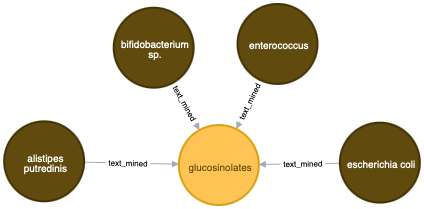
\includegraphics[width=6in]{figs/glucosinolate_to_bacteria.png}
\par\end{centering}}
\caption[Glucosinolates to Bacteria]{\label{Fig_glu_to_bac} A graph from the ABCkb 2.0 showing the connectivity from glucosinolates to bacteria.}
\end{figure}

%% Andrew Neilson's publications
%% https://scholar.google.com/citations?hl=en&user=qlXsJxgAAAAJ&view_op=list_works&sortby=pubdate

To explore connections between \textit{A. putredinis} and phenotypes, a knowledgebase query was constructed in the ABCkb from \textit{Alistipes putredinis} to phenotype (Figure ~\ref{Fig_ali_to_pheno}). Connections from the Disbiome database indicate manually curated connections from \textit{Alistipes} to phenotype and text-mining revealed an additional connection to obesity. This connection was from a study tracking weight loss patients over time and found that \textit{Alistipes} abundance is negatively correlated with obesity\cite{louis_characterization_2016}. Given the disbiome connection between \textit{A. putredinis} and reduction of liver cirrhosis, the link between this bacterium and obesity is logical. Non-Alcoholic Fatty Liver Disease (NAFLD) is linked with incidences of obesity along with many metabolic disorders like hypertension, type 2 diabetes, and hypertension \cite{sarwar_obesity_2018}. 

\begin{figure}[!h]
{\begin{centering}
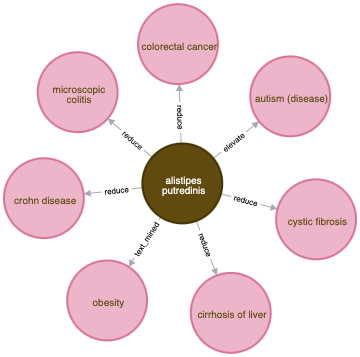
\includegraphics[width=6in]{figs/ali_to_pheno.png}
\par\end{centering}}
\caption[Glucosinolates to Bacteria]{\label{Fig_ali_to_pheno} A graph from the ABCkb 2.0 showing the connectivity from glucosinolates to bacteria.}
\end{figure}

What then would be the molecular mechanisms driving the interaction between \textit{A. putredinis}, obesity, and connected metabolic disorders such as cirrhosis of the liver? The previously explored path between glucosinolates, the cytochrome P450 gene, and arachidonic acid metabolism provides a possible explanation between this link. Hydroxyeicosatetraenoic acids produced from the arachidonic acid metabolic pathway, not the pathway attributed to glucosinolates is linked with obesity \cite{pickens_obesity_2017}. Therefore it is plausible that gut microbiota perform the activation
step, like myrosinase, necessary to yield the protective benefits and explains the connection between \textit{A. putredinis} and obesity. This should be further explored.

\subsection{Resveratrol, Akkermansia, and diabetes}

Abundances in the gut of bacterium in the Akkermansia genus have been linked to many favorable health outcomes (Figure \ref{akkermansia}) \cite{naito_next-generation_2018}. Specifically metabolic-related health outcomes, such as weight management and diabetes, are found to be inversely linked to abundances of \textit{Akkermansia muciniphila}\cite{dao_akkermansia_2016}. This bacterium is gram-negative, oval-shaped, and lives in the mucosal layer of the gut along with several other places in the human body like the small intestine, human milk, and the mouth \cite{geerlings_akkermansia_2018}. \textit{Akkermansia} degrades mucin within the gut and produces Short Chain Fatty Acids (SCFAs), compounds often linked with gut health\cite{blaak_short_2020,derrien_akkermansia_2004}. While this may sound negative, and was previously considered detrimental, it is in fact a positive, normal process\cite{van_herreweghen_mucin_2018,norin_establishment_1985}. One SFCA in particular, butyrate has been shown to upregulate goblet cell mucin production in the gut through interaction with MUC genes \cite{gaudier_butyrate_2004}. In addition, butyrate and other SFCAs are linked to the increase of other beneficial bacteria in the gut, and the gut-brain axis\cite{jiminez_butyrate_2017,silva_role_2020}. Therefore, it is likely that increasing \textit{Akkermansia} would subsequently increase SFCA production in the gut which would lead to more mucin production, and ultimately a healthier gut microflora. However, the molecular mechanism by which \textit{Akkermansia} affects human health is still an avenue of exploration. In the ABCkb, Akkermansia is linked to 54 different Phenotype nodes. Of those 54 nodes, 4 are related to diabetes and metabolic disorders (Figure. \ref{Fig_akker_to_pheno}). Links between \textit{Akkermansia} and polyphenol-rich diets have been established\cite{anhe_triggering_2016}.

\begin{sidewaysfigure}[!h]
{\begin{centering}
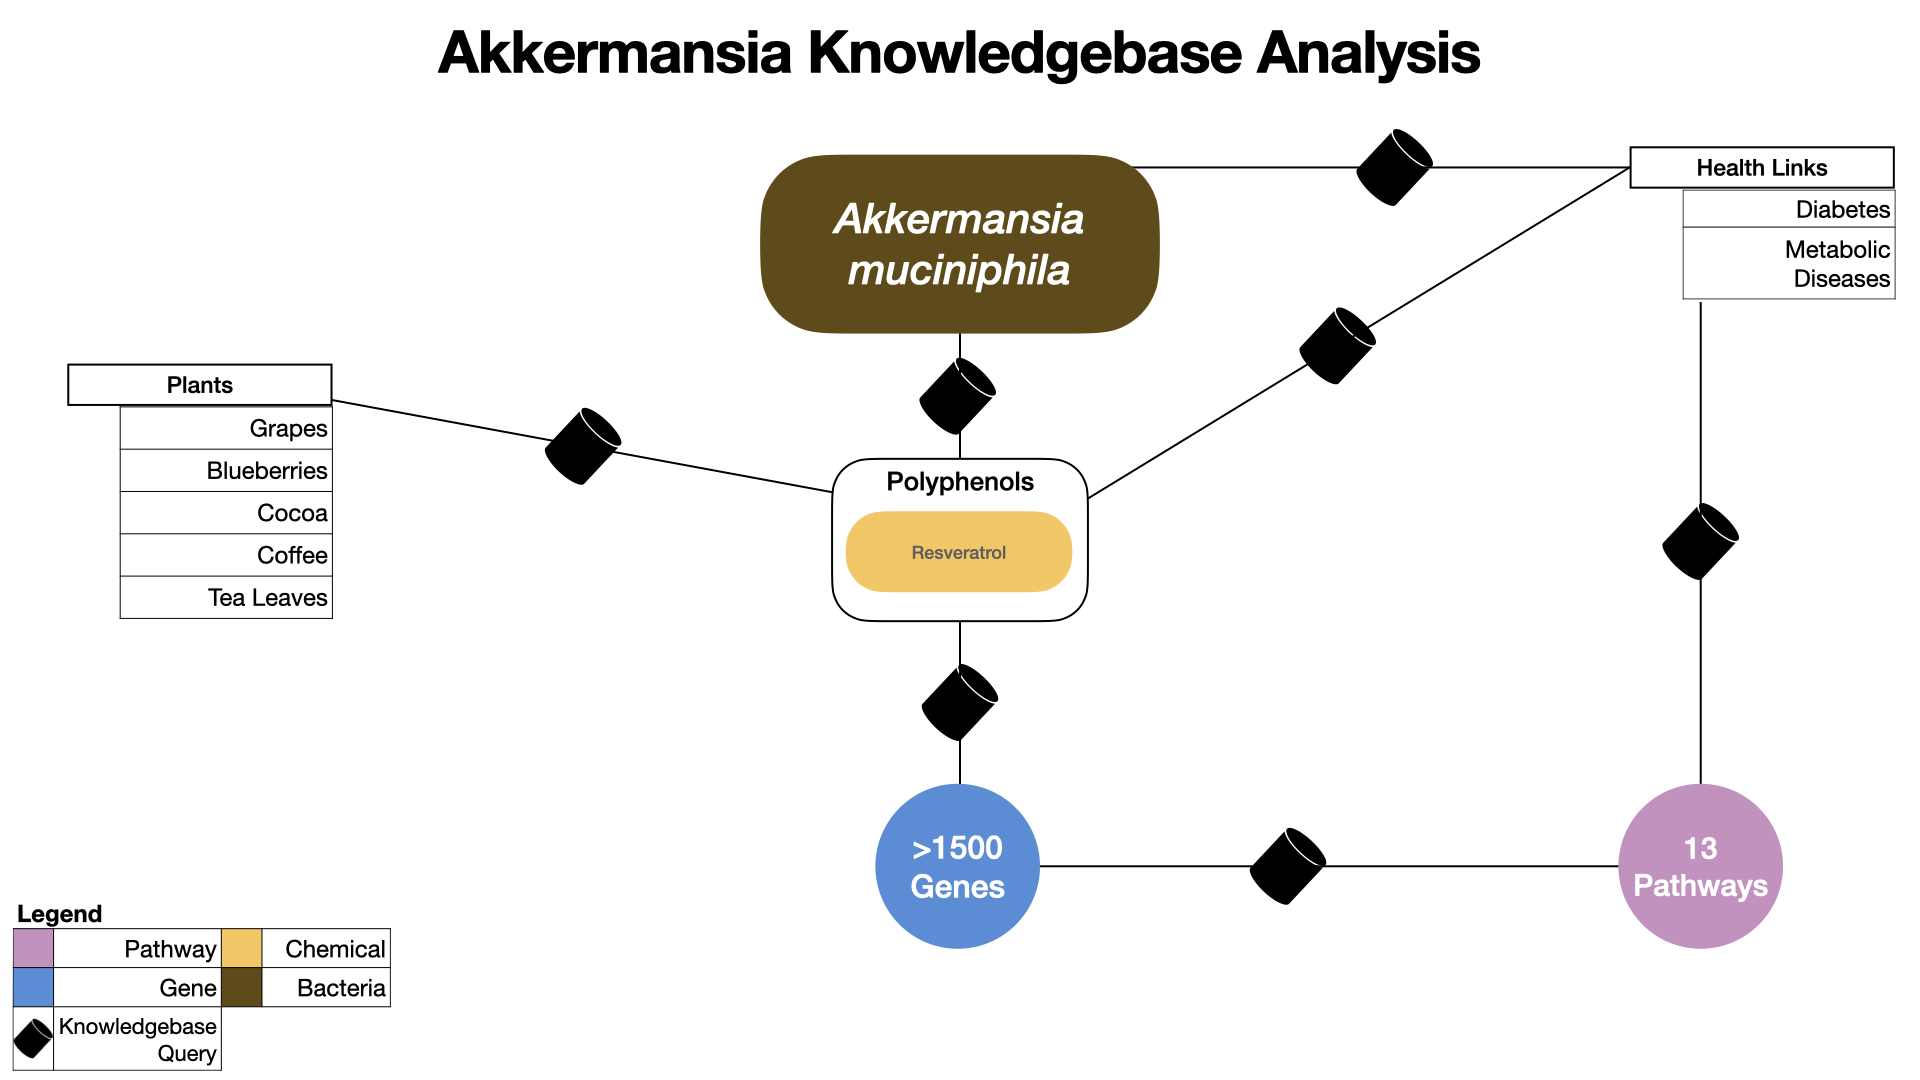
\includegraphics[height=5in]{figs/akkermansia.png}
\par\end{centering}}
\caption[Akkermansia knowledgebase overview]{\label{akkermansia} The overview of the knowledgebase analysis explaining the connection between \textit{Akkermansia muciniphila}, diabetes, and metabolic disorders }
\end{sidewaysfigure}

\begin{figure}[!h]
{\begin{centering}
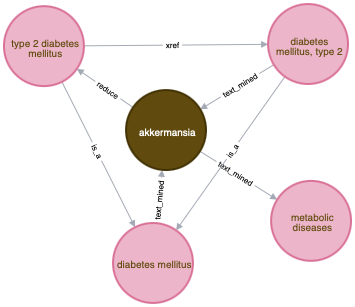
\includegraphics[width=6in]{figs/akker_to_phe.png}
\par\end{centering}}
\caption[Akkermansia to metabolic disorders]{\label{Fig_akker_to_pheno} A graph from the ABCkb 2.0 showing the connectivity from Akkermansia to metabolic disorders and type 2 diabetes.}
\end{figure}

The foods that contain polyphenols include grapes, blueberries, coffee, tea, and cocoa powder\cite{perez-jimenez_identification_2010}. These foods with their polyphenolic compounds are attributed to a host of health effects\cite{joven_polyphenols_2014, cory_role_2018}. In the ABCkb, Akkermansia is linked to 74 Chemicals, of which polyphenols are prevalent (Figure. \ref{Fig_akker_to_che}). One specific polyphenol, resveratrol found primarily in berries, is released in response to plant stressors like pests and infections\cite{jeandet_regulation_2019}. 

\begin{figure}[!h]
{\begin{centering}
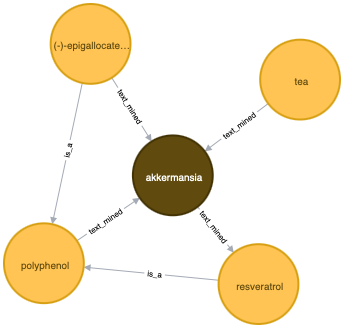
\includegraphics[width=6in]{figs/akker_to_che.png}
\par\end{centering}}
\caption[Akkermansia to polyphenols]{\label{Fig_akker_to_che} A graph from the ABCkb 2.0 showing the connectivity from Akkermansia to polyphenols.}
\end{figure}

Resveratrol is the primary compound that gives red wine its claimed health benefits. In the ABCkb, resveratrol is linked to 3,866 genes, 93 more than the Comparative Toxicogenomics Database has available \cite{davis_comparative_2019}. There are 13 pathways related to glucose and insulin with over 1500 genes between (Table \ref{tab:path2resv}).

\begin{table}[H]
\begin{centering}
\centering
{\small{}}%
\begin{tabular}{|c|c|c|}
\hline
{\small{}Gene Count} & {\small{}Pathway Name} & {\small{}Pathway ID}\tabularnewline
\hline
\hline
{\small{}899} & {\small{}Insulin Secretion} & {\small{}GO:0030073}\tabularnewline
\hline
{\small{}426} & {\small{}Glucose Metabolic Process} & {\small{}GO:0006006}\tabularnewline
\hline
{\small{}382} & {\small{}Glucose Import} & {\small{}GO:0046323}\tabularnewline
\hline
{\small{}295} & {\small{}Glucose Homeostasis} & {\small{}GO:0042593}\tabularnewline
\hline
{\small{}216} & {\small{}Gluconeogenesis} & {\small{}GO:0006094}\tabularnewline
\hline
{\small{}136} & {\small{}Insulin Receptor Signaling Pathway} & {\small{}GO:0008286}\tabularnewline
\hline
{\small{}24} & {\small{}Insulin Catabolic Process} & {\small{}GO:1901143}\tabularnewline
\hline
{\small{}23} & {\small{}Insulin Metabolic Process} & {\small{}GO:1901142}\tabularnewline
\hline
{\small{}18} & {\small{}Glucocorticoid Secretion} & {\small{}GO:0035933}\tabularnewline
\hline
{\small{}10} & {\small{}Insulin Processing} & {\small{}GO:003070}\tabularnewline
\hline
{\small{}10} & {\small{}Positive Regulation of Glucokinase Activity} & {\small{}GO:0033133}\tabularnewline
\hline
{\small{}6} & {\small{}Renal Glucose Absorption} & {\small{}GO:0035623}\tabularnewline
\hline
{\small{}4} & {\small{}Insulin Receptor Internalization} & {\small{}GO:003816}\tabularnewline
\hline
\end{tabular}
    
\par\end{centering}{\small \par}
\caption[Pathways connected to resveratrol]{\label{tab:path2resv} The pathways connected to resveratrol related to glucose and insulin with the gene counts in-between.}
% match p=(b:Chemical)--(a:Gene)--(c:Pathway)--(d:Phenotype) where b.name = 'resveratrol' and d.name in ["diabetes mellitus, type 2", "metabolic diseases", "diabetes mellitus", "type 2 diabetes mellitus"] and c.name =~ ".*luco.*" or c.name =~ ".*nsuli.*" return count(distinct a) as gene_count, c.name, c.xref order by gene_count des
\end{table}

The generalized links between diabetes and resveratrol may be fully explained by the interaction between \textit{Akkermansia} and resveratrol. This connection should be further explored to elucidate the effect of dietary polyphenols on \textit{Akkermansia}.

\section{Discussion}

Generating these connections manually through intense literature reviews adds significant time burdens to overburdened researchers. This knowledgebase however provides the nutritive connections in papers in a graphical, browsable format, with references for clear knowledge of where the associations are derived, and where to go to explore the study that produced the association. In addition, the size of the knowledgebase is a manageable 2.8 Gigabytes, over the 50 Gigabyte version original.

There are a few limitations to this knowledgebase and method of creation. The first is the availability, and the significant time component of obtaining permissions to mine through full text articles. During our quest to obtain access for full-text mining, publishers often expressed concern that a knowledgebase like this would reduce the number of journal readers. We propose that this knowledgebase and others like it would in fact increase journal readers as they discover the nutritive connections within articles and desire to probe further. Methods sections often house additional information pertinent to experimental design not contained within the knowledgebase. The ABCkb merely expedites the literature review process and can point to more relevant results. Queries for \textit{Alistipes} in the NCBI pubmed repository return several results irrelevant to nutrition. Custom MeSH queries reduce the overall papers returned but the researcher is left to read each one of the papers to find the associations within. With a restriction of papers, there is a question of how much text is too much. In the \textit{Alistipes} to obesity example, the text-mining result was in fact found in a paper examining different methods for analyzing microbiome count data which referenced the original study that we did not have access to text-mine \cite{zhang_negative_2017}. In a case where not all texts are available to mine through, assertions can be found from texts that reference other texts. Future work could expand on this knowledgebase to rank associations and articles of interest based on similar reference sections. Abstracts and references are often freely browsable. Mining through abstracts to extract associations and then following up with a ranking method to rank related articles could provide researchers with additional articles to read for further information.
%%(something about ranking results through pagerank if multiple matches were found)

Another limitation to this knowledgebase is the method by which the results were obtained. Rule and dictionary approaches work well for mining through literature sources where the dictionaries are well-defined, however microbiome literature is a metaphorical wild-west. When bacteria are taxonomically reclassified, connecting old bacteria names to the reclassified name is a significant challenge. In addition, bacteria are referred to in some studies with an informal moniker to designate multiple strains. Connecting these associations may be possible through some complicated regular expression checking or a true machine learning approach may be required.

Finally the desire to probe drug compounds and their relation to the plant molecular mechanism pathway has been expressed. Nutrichem 2.0 included drugs and some of their effects in their database \cite{ni_nutrichem_2017}. One common example is the ability for grapefruit to reduce the efficacy of some heart medications \cite{bailey_interactions_2004}. Similar effects with different drugs have been seen in people with varying microbiota abundances.

\section{Conclusion}

This knowledgebase, the ABCkb 2.0, further expands on the original knowledgebase with the addition of microbiome connections and dietary connections. Text-mining full-text articles extracted more associations than abstracts, but also requires more strict filtering. Two knowledgebase analyses were produced to demonstrate the effectiveness of the ABCkb and the potential to generate testable hypotheses. Further work on this should validate the associations within through physical assays.


\chapter{APPLICATION OF KNOWLEDGEBASED-DISCOVERY TO THE SARS-CoV-2 PANDEMIC AND DEVELOPMENT OF THE COVID TO DIET KB (CDkb)} % REWRITE!

Coronaviruses are prevalent in nature and are responsible for various respiratory infections, many of which are non-life threatening \cite{vkovski_coronavirus_2021}. They spread among bat populations and the first significant coronavirus infection with a high mortality rate was first identified in 2003 after it spread in a hotel \cite{rastogi_sars_2020}. This coronavirus was named SARS-CoV-1 which stands for Severe Acute Respiratory Syndrome CoronaVirus 1. It took a significant effort to achieve sequencing and many hours of work \cite{marra_genome_2003,noauthor_cdc_nodate}. Fortunately the spread of the virus was mitigated, however experts continued to study the virus and the effect on the human body. In 2008 another coronavirus appeared in the middle-east and was named MERS-CoV. Finally, in late 2019 a coronavirus began to spread in the Wuhan province of China which reached pandemic proportions within a few months \cite{vkovski_coronavirus_2021}. Technological advances led to a quick identification of the virus, and SARS-CoV-2 was the culprit. While our previous knowledgebases have been applied to noncommunicable diseases caused by dietary or genetic factors, communicable diseases of pandemic proportion will benefit from this method.

\section{Background}

% Coronaviruses
% - phenotypic characteristics

Coronaviruses are positive-sense RNA genome, circular viruses that exist in abundance in nature \cite{vkovski_coronavirus_2021}. The SARS-CoV-2 genome is around 30 kb which makes it one of the largest in the class of RNA viruses\cite{rastogi_sars_2020}. Covering the exterior of coronaviruses is a lipid bilayer envelope with three protein types (membrane, envelope, and spike) protruding out from the surface\cite{yuki_covid-19_2020}. In SARS-CoV-2, viral infection is facilitated through the spike protein binding to ACE2 receptors on host cells\cite{scudellari_how_2021}. Infection is further enhanced through its host immune system evasive detection measures through utilization of glycan molecules that coat the spike proteins\cite{scudellari_how_2021}. This coating limits host T-cell activation. While some general pathology was known prior to the pandemic, from other coronavirus studies, much of this information was discovered and broadly communicated through preprint articles\cite{fraser_evolving_2021}.

% The publishing path of all of the pre-print articles
% - How there were so many so quickly

The acceptance of pre-print article servers and repositories is still somewhat controversial \cite{sheldon_preprints_2018}. Traditional scientists dislike pre-print articles due to the fact that peer-review is the stage-gate that reduces the spread of bad science. The process of review identifies and removes faulty experiment methods, unfounded results, and poor writing, which overall increases the quality of published literature \cite{carneiro_comparing_2020}. In contrast, modern scientists argue that the large volume of papers being submitted for publication overwhelms the peer-review process and delays scientific progress. The process can be expedited but that requires reviewers pre-selected for journal topics that are in demand or of focus. It is argued that preprinted articles are able to be reviewed by a wider panel of scientists in the community \cite{fry_praise_2019}. Additionally, peer-reviewing is not as strict of a stage-gate as believed. A study found that articles can be passed through peer-review using language generated from computational methods \cite{van_noorden_publishers_2014}. Pre-print servers then exist to spread scientific information in an expedited manner while still honoring the process of peer-review. 

The utility of pre-print articles was seen early in the pandemic. An average of 39.5 pre-print articles were circulated per day during the pandemic and by 6 months, over 6,000 articles were available\cite{brierley_lessons_2021,fraser_evolving_2021}. An additional factor to consider in the flow of information is the technological progress that has been made since the previous coronaviruses. The sequence for SARS-CoV-2 was available much sooner than for SARS-CoV-1, and MERS-CoV (Figure \ref{fig_sars_compare}). 

\begin{figure}[!h]
    {\begin{centering}
    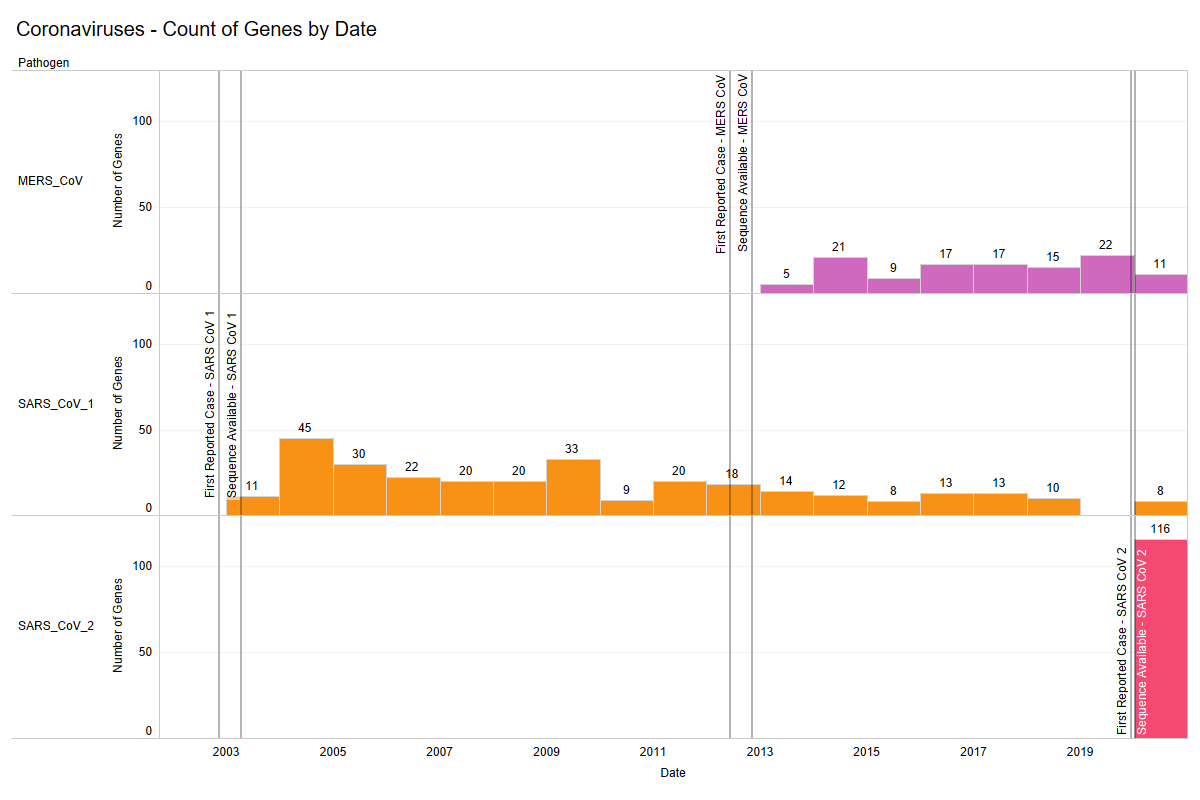
\includegraphics[width=6in]{figs/Timeline.png}
    \par\end{centering}}
    \caption[Rate of gene connections and sequence availability between 3 coronaviruses]{\label{fig_sars_compare} A comparison between the three major coronavirus contagion sequence availabilities and amount of genes linked to each individual pathogen by year, generated 6 months after the start of the pandemic.}
\end{figure}

A weekly updated preprint repository was set up specifically for SARS-CoV-2 papers, along with the peer-reviewed papers on the relative coronaviruses \cite{lu_wang_cord-19_2020}. The pre-printed articles in this repository also came with reviewer comments on the articles for researchers to identify any areas of concern and mitigate any false information. All documents in the repository were provided in JavaScript Object Notation for convenient processing by text-mining tools. As the pandemic progressed, one symptom seen in a notable portion of infected patients is a prolonged infection of SARS-CoV-2.

One of the challenging parts of the pandemic was the broad range of symptoms present in infected individuals \cite{yuki_covid-19_2020}. Some patients had symptoms similar to a cold, where others presented more severe symptoms. Infections in many cases led to a condition called COVID-pneumonia which resulted in patients requiring supplemental oxygen. In severe circumstances patients had to be sedated and placed on a ventilator. Once patients conquered the initial infection, many were left with a condition called long-covid \cite{maltezou_post-covid_2021}. This condition persists for several months following the initial infection and presents with myalgia-like symptoms along with mild symptoms present in the initial infection: anosmia, ageusia, and difficulty breathing. Survival rates of SARS-CoV-2 infections were linked to noncommunicable patient comorbidities like type 2 diabetes (T2D), heart disease, and obesity\cite{djaharuddin_comorbidities_2021}. These comorbidities are all diet-related. Therefore, diet alteration and subsequent reduction of patient comorbidities is of great interest. This knowledgebase was built to explore and build hypotheses around the molecular mechanisms between pathogen and plant phytochemical metabolic pathways.


\section{Building the CDkb}

The Covid to Diet knowledgebase (CDkb) was built from the original ABCkb 1.0 with the addition of associations from the CORD-19 dataset and drug information from the drugbank database (Figure \ref{Fig:cdkb_arc}) \cite{lu_wang_cord-19_2020,wishart_drugbank_2008}. 

\begin{figure}[!h]
    {\begin{centering}
    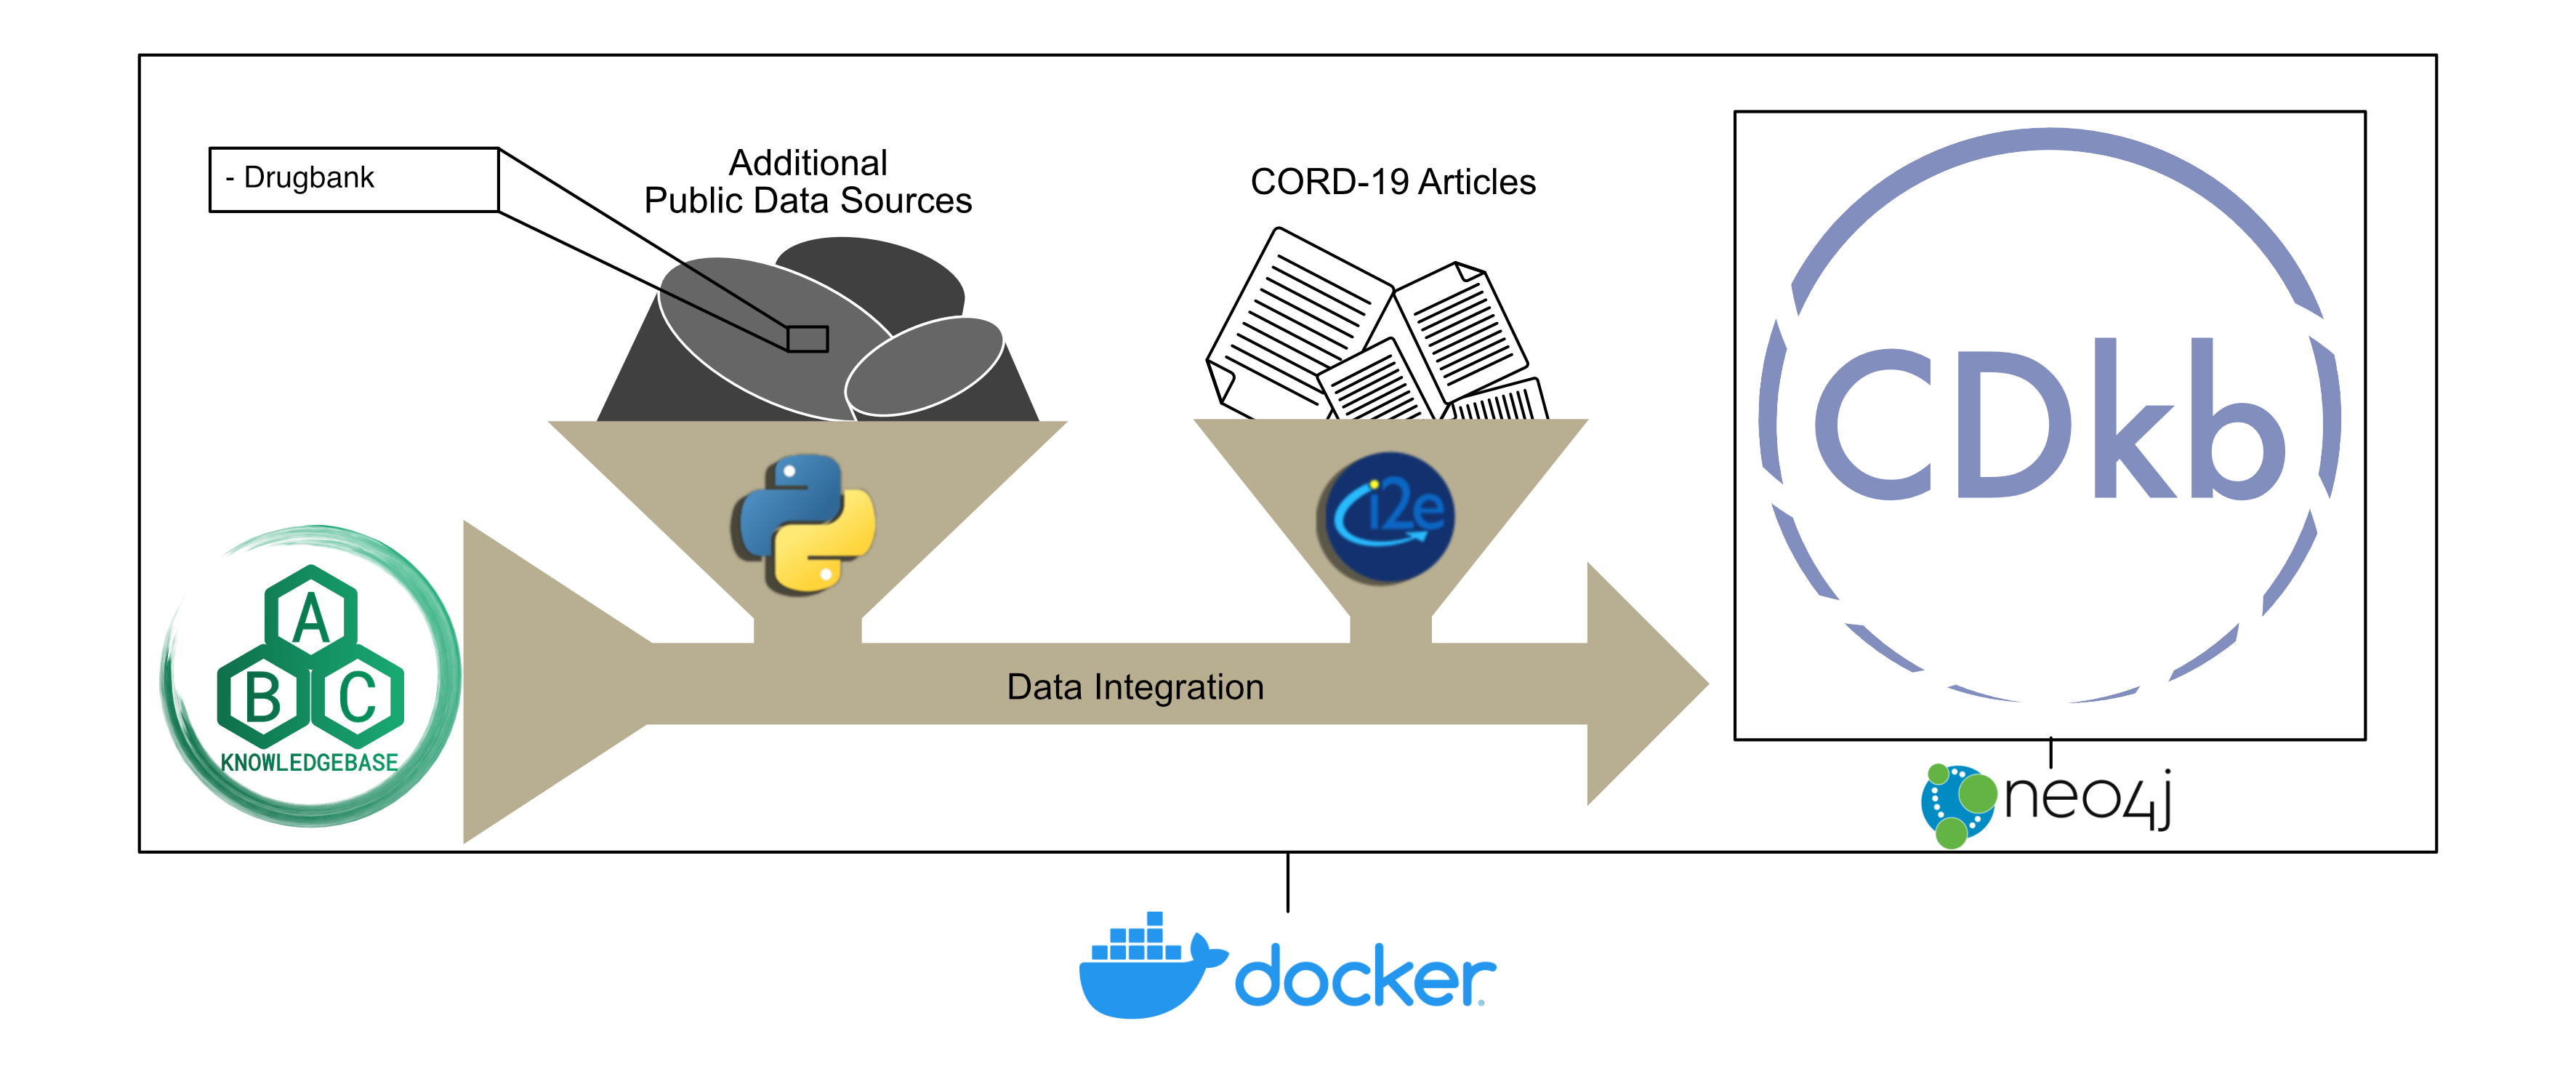
\includegraphics[height=2.5in]{figs/cdKB_architecture.png}
    \par\end{centering}}
    \caption[CDkb Architecture]{\label{Fig:cdkb_arc} The process of creating the CDkb starts with the original knowledgebase and adding drugbank information with text-mined information from the CORD-19 dataset.}
\end{figure}

\subsection{Structured data sources}

Data in the CDkb comes from the original 11 sources from the ABCkb 1.0 with the addition of drug information. Though drugs are technically a subset of chemicals, within this knowledgebase they are marked as a separate set of nodes. This allows for more efficient queries for open-discovery with drugs as the starting point. Drugs from the drugbank database were parsed and added to the knowledgebase with connections to genes from the original ABCkb\cite{wishart_drugbank_2008}. Then text mined associations from I2E were added to the knowledgebase.

\subsection{Natural Language Processing Relationships between Viruses and Human genes}

A subset of literature from the CORD-19 dataset updated in July, 2021 with preprinted research, papers from Elsevier corpii and other Pubmed Central articles was downloaded and converted from jsonified text to xml for indexing in I2E\cite{lu_wang_cord-19_2020}. This conversion was done through a custom python script and extracted sections where they were available within the original json header. When sections were unavailable, the text was labeled "general." The preprinted subset contained articles with reviewer comments, which was not useful for our immediate use and increased duplicate hits. To reduce unnecessary duplicate text-mined results, matches from the files containing reviewer comments were negated by removing any  Additionally, any matches from methods and reference sections were negated. Articles were grouped into batches and uploaded to the server with the I2E interface.

After indexing, text-mining queries from I2E from the "class affects class" subset were run and refined to identify hits where SARS-CoV-1, SARS-CoV-2, or MERS-CoV affect human genes. An ontology of predicates provided by Linguamatics was used to link the Coronavirae to human genes in the literature. All of this information was inserted into a Neo4j graph database in a Docker container (Figure \ref{Fig_4_1}). 

\begin{sidewaysfigure}[!h]
    {\begin{centering}
    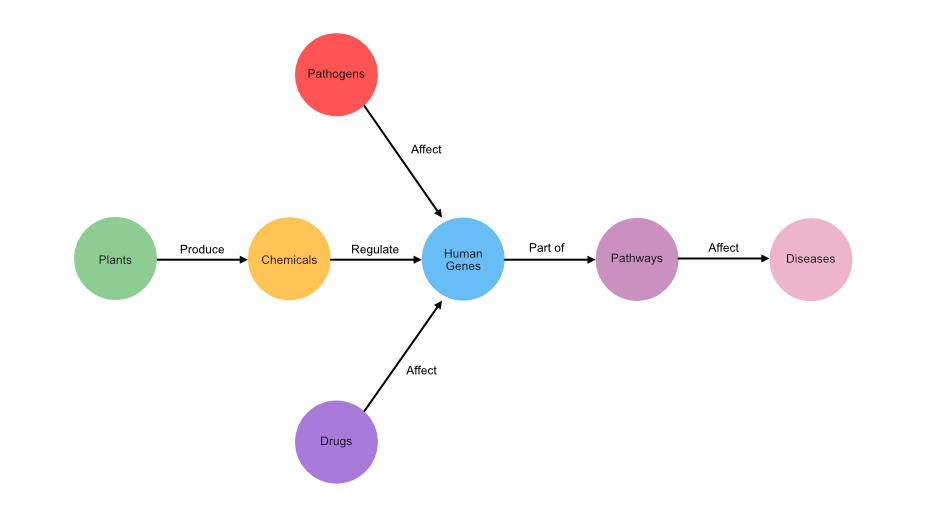
\includegraphics[height=4.5in]{figs/KB_outline_w_covid.png}
    \par\end{centering}}
    \caption[CDkb schema]{\label{Fig_4_1} The schema for the CDkb showing connectivity to the elements from the ABCkb 1.0}
\end{sidewaysfigure}

% \section{Examining extracted relationships}

% Relationships between SARS-CoV-1, SARS-CoV-2, and MERS-CoV will be examined to determine pathway hits and compare the preliminary results of the novel strain to the established knowledge of the two previous strains. 

\subsection{Projecting genes on pathways}

Pathview is a tool produced to visually display heatmap gene expression values on KEGG pathways \cite{luo_pathview_2013}. We used Pathview to map text-mined gene hits between strains to determine top pathways identified and visualize gene hits on pathway maps. We also compared two methods: using the raw number of hits identified from text-mining, as gene expression values, or calculating a modified TF/IDF score. Raw hit scores are computed as the sum of gene hits per strain. Limitations of using raw hits as a metric for comparing gene hits across strains is the obvious discrepancy in corpus size given a short time-frame for papers on SARS-CoV-2 vs MERS-CoV and SARS-CoV-1. A TF/IDF score is commonly used to mitigate this limitation. The TF/IDF score is calculated from two separate values: Term Frequency, and Inverse Document Frequency. TF(T,D) is calculated as the number of times the term (T) is found in a document (D) \ref{eq:TF}. IDF(T) is calculated from taking the logarithm of the number of documents N, divided by the sum of documents containing term (T) (\ref{eq:IDF}). These two values are multiplied together to produce a score indicating importance, irrespective of frequency. Pathview allows us to map identified genes in pathway maps from the Kyoto Encylopedia of Genes and Genomes (KEGG) and visualize the strains together to determine the most relevant pathways, given the preliminary research.

\begin{equation}
TF(T,D) = f_{T,D}
\label{eq:TF}
\end{equation}

\begin{equation}
IDF(T) = log\frac{N}{|\{d \in D : T \in d\}|}
\label{eq:IDF}
\end{equation}

\begin{equation}
TF\-IDF = TF * IDF
\label{eq:TFIDF}
\end{equation}

% \subsection{Grouping functionally annotated genes}

% To group functionally annotated genes, we utilized the Database for Annotation, Visualization and Integrated Discovery (DAVID) resource. This tool provides grouping and analysis of related genes into GO pathways. GO pathways are currently the source of pathway information within the ABCkb and will provide a connection both to human phenotypes and plants with their phytochemicals to examine nutritive associations. 

\subsection{Exploring nutritive associations}

Nutritive associations built in the ABCkb provide a link from plants to their phenotypes. After mapping COVID-19 associations, we probed possible molecular mechanisms linked with viral infections, along with long-covid infections. Additionally, dietary habits may exacerbate viral infections by up-regulating or down-regulating genes necessary for mounting an immune response. Dietary phytochemical connections were also explored to produce a knowledgebase analysis.

\section{Results}

\subsection{Text-Mined Results}

The I2E text-mining query extracted 232,595 associations between the three Coronaviruses and host factors (Genes). Text-mining revealed over 4,000 host factors between these 3 coronaviruses with 1500 common host factors between SARS-CoV-1 and SARS-CoV-2 (Figure \ref{Fig_covid_2hf}). This is over two-times the host factors mined from SARS-CoV-2 and MERS-CoV. These associations were found in over 49,000 articles with an average of 10 documents to each gene (Figure \ref{Fig_dist_hf}).

\begin{figure}[!h]
    {\begin{centering}
    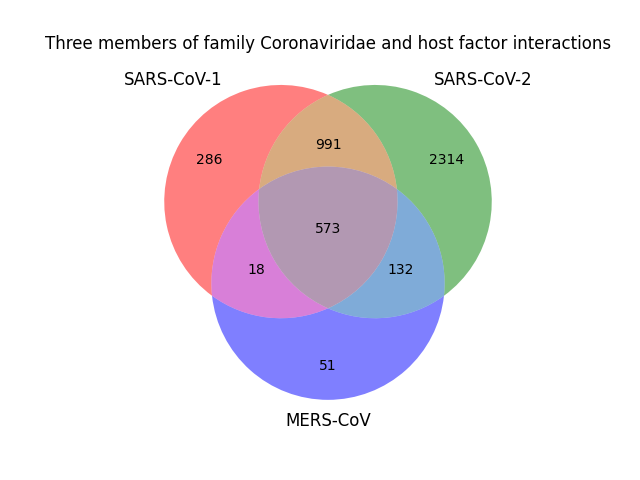
\includegraphics[height=4.5in]{figs/covid2hf.png}
    \par\end{centering}}
    \caption[Coronaviridae and host factor intersections]{\label{Fig_covid_2hf} The intersection between 3 members of the family Coronaviridae and the text-mined host factor interactions from CORD-19}
\end{figure}

\begin{figure}[!h]
    {\begin{centering}
    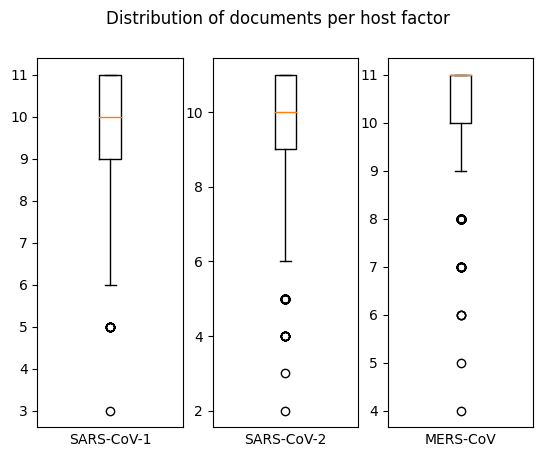
\includegraphics[height=4.5in]{figs/boxplot_hit.png}
    \par\end{centering}}
    \caption[Distribution of documents to host factor]{\label{Fig_dist_hf} The distribution of documents to host factor identified through I2E text-mining with an average of 10 documents per host factor.}
\end{figure}

\subsection{Knowledgebased discovering molecular mechanisms of long-covid}

Long-COVID, or post-COVID syndrome is a range of symptoms experienced by patients four months beyond the initial SARS-CoV-2 infection\cite{raveendran_long_2021}. The current range of symptoms of post-covid symptoms includes many of the symptoms experienced in the initial infection with additional mental and cognitive symptoms, along with symptoms that increase with physical exertion\cite{aiyegbusi_symptoms_2021}. A cursory glance at the literature reveals many pathways that may result in experiencing these symptoms after infection.

There are several possible routes to generate a hypothesis around long-covid molecular mechanisms. As the symptoms are broad and seemingly disconnected, we began the knowledgebase search with known symptoms unique to long-covid (Figure \ref{lc_analysis}. This search revealed a set of 29 phenotypic nodes from 9 symptoms (Appendix Table \ref{tab:lcphen}). These phenotypic nodes alone are linked with 218 pathways and 36,369 gene nodes. There are 1,453 genes in the intersection of the text-mined host factors linked to SARS-CoV-2 in the CDkb and the genes connected with these 29 phenotypic nodes.

\begin{sidewaysfigure}[!h]
    {\begin{centering}
    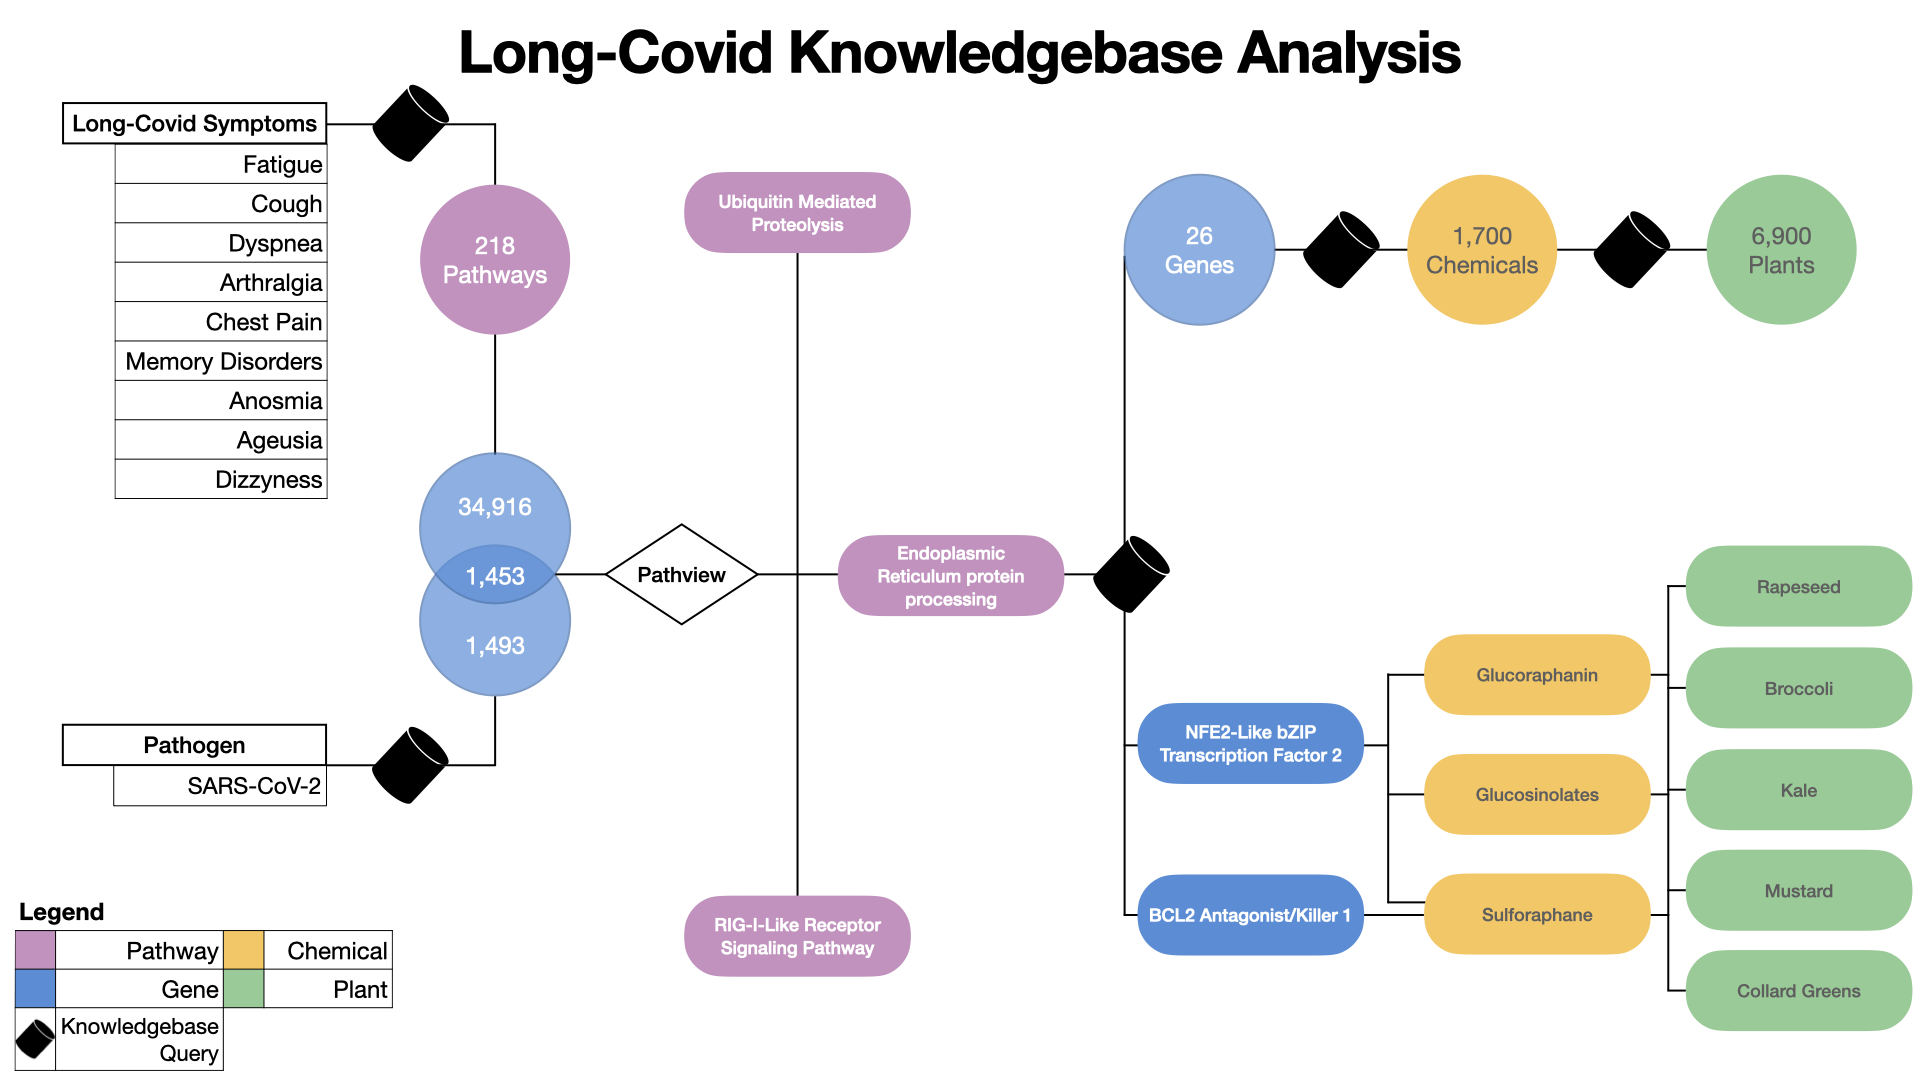
\includegraphics[height=5in]{figs/long_covid_knowledgebase_analysis.png}
    \par\end{centering}}
    \caption[Long-Covid Knowledgebase Analysis]{\label{lc_analysis} The high-level overview of the knowledgebase analysis around long-covid and the hypothesised plants and phytochemicals with possible alleviation}
\end{sidewaysfigure}

With the filtered genes from the knowledgebase, we performed a Pathview pathway analysis with the calculated TF*IDF scores from text-mining \cite{luo_pathview_2013}. Using automatic pathway selection which filters KEGG pathways to the most relevant pathways between the 3 Coronaviridae types. This analysis produced three KEGG pathway maps: Ubiquitin Mediated Proteolysis (Appendix Figure \ref{Fig:Pathview_ub}), Protein Processing in Endoplasmic Reticulum (Figure \ref{Fig:Pathview_pro}), and RIG-I-Like Receptor Signaling Pathway (Appendix Figure \ref{Fig:Pathview_rig}). Each map indicates the genes identified through text-mining with the TF*IDF scores providing color. Additionally, gene blocks are segmented by coronaviridae in order (left to right): SARS-CoV-1, SARS-CoV-2, MERS-CoV. One specific pathway of interest from the Pathview analysis is the Endoplasmic Reticulum Protein Processing pathway. This pathway is involved in protein folding within the cell.

\begin{sidewaysfigure}[!h]
    {\begin{centering}
    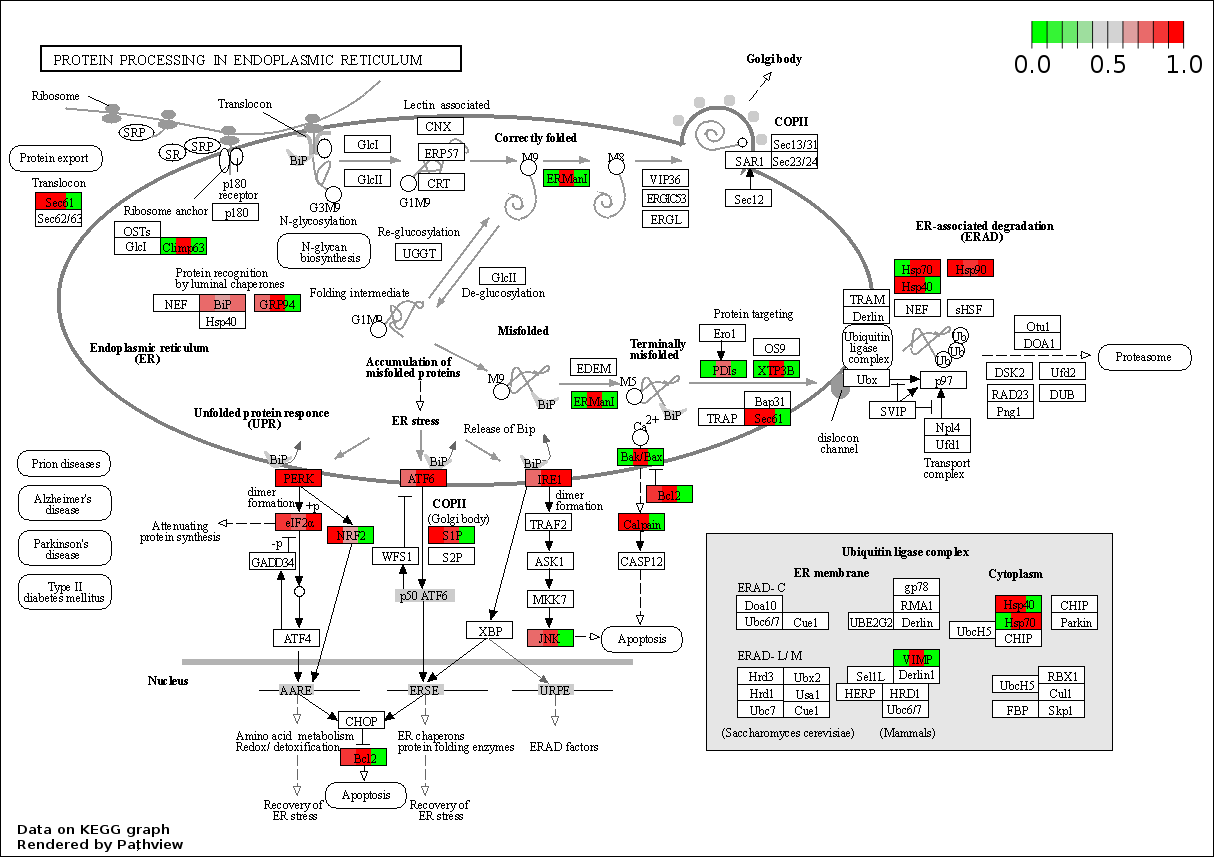
\includegraphics[height=6in]{figs/hsa04141.png}
    \par\end{centering}}
    \caption[Pathview Protein Processing in Endoplasmic Reticulum and TM Hits]{\label{Fig:Pathview_pro} The hits from the pathview analysis with TF*IDF scores providing color values with the 3 coronaviridae. Colored gene boxes from left to right are: SARS-CoV-1,SARS-CoV-2,MERS-CoV}
\end{sidewaysfigure}

Synthesized proteins are exported through the Endoplasmic Reticulum (ER) for cutting, folding, shaping and other modifications \cite{stevens_protein_1999}. These modifications are facilitated by a set of molecular chaperones and enzymes that ensure correct protein folding and export the protein to the golgi body for any additional post-translational modifications \cite{braakman_protein_2013}. The ER employs a series of accuracy checks before exporting the protein which ensures that the protein has been folded, folded properly, or needs to be degraded. ER stress is caused by a multiplicity of factors. Under stress, cascading pathways lead to either the adjustment of ER processing, stimulation of endoribonuclease activity, attenuation of cell translation, or signaling apoptosis of the cell \cite{adams_structure_2019}. From the Pathview analysis, there are several genes in these cascading pathways highlighted under protein stress, which is expected given the mechanism of viral production. Three genes of interest are eukaryotic translation initiation factor 2 alpha kinase 3 (PERK), endoplasmic reticulum to nucleus signaling 1 (IRE1), and activating transcription factor 6 (ATF6). 

Traditional myalgias include Chronic Widespread Pain (CWP) and Fibromyalgia Syndrome FMS \cite{olausson_protein_2015}. These are considered syndromes due to there being no clear disease pathway identified and the broad spectrum of symptoms that are selectively experienced by patients. Many of the symptoms experienced by patients with myalgias are also experienced in long-covid patients. In one study, myalgia patients have been found to experience severe pain hypersensitivity which is linked to widespread production of advanced oxidative protein products, formed in response to oxidative stress that lead to cellular apoptosis \cite{ding_advanced_2017}. One specific gene drawn out from that study is the mitogen-activated protein kinase 8 (JNK) gene, highlighted in the graph and downstream from the IRE1 mediated cascade. Links between myalgias, blood coagulation pathways, and immunity pathways have also been shown \cite{wahlen_plasma_2018}. Other evidence shows that microclots are found in long-covid patients, which mirrors what is known of apoptotic cells and the affect on procoagulation pathways\cite{yang_procoagulant_2017, pretorius_persistent_2021}. Therefore, it is possible that a high level of infection, leading to ER stress and widespread apoptosis, facilitated by increased IRE1 gene activation, causes long-term symptomatic periods for patients following SARS-CoV-2 infection. As syndromes like CWP and FMS have no definitive test to confirm diagnoses, testing for increases in clotting factors or microclots may provide a path forward for diagnosing patients.

\subsection{Knowledgebased discovery of nutritional myalgia-like symptom mediation in long-covid patients}

Mediation and reduction of long-covid symptoms that mirror myalgia symptoms often follows a course of Selective Serotonin Reuptake Inhibitor (SSRI) drugs in conjunction with pain reduction drugs like Tylenol or Ibu-profen \cite{oskotsky_mortality_2021}. However there may be nutritive pathways that alleviate the underlying molecular mechanisms driving the experience of symptoms. Using the identified genes in the ER protein processing pathway as initial start points, a knowledgebase query was developed to identify possible nutriceutical phytochemicals.

There are over 1,700 phytochemicals linked to over 6,900 plants in the Covid to Diet Knowledgebase. As the links between leafy green vegetables, and members of the brassica family, to heart health is well established, we started with those. Two of the genes in this pathway that lead to apoptosis are linked with glucosinolates, and sulforaphane (Figure \ref{cov_gene2chem}). These compounds are found in vegetables in the brassica family like Broccoli, Collard Greens, and Cabbage. Sulforaphane has been found to affect seratonin release, which increases the strength of this connection \cite{mastrangelo_serotonin_2008}. If widespread systemic cellular ER stress causes experience of myalgia symptoms in long-covid patients, the CDkb indicates that increased consumption of glucosinolate vegetables may provide relief through the mentioned molecular mechanisms. This connection should be explored further. 

\begin{sidewaysfigure}[!h]
    {\begin{centering}
    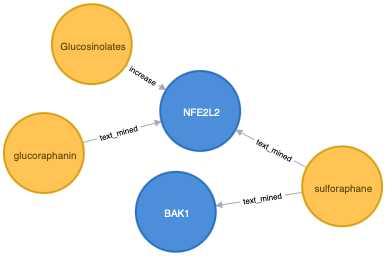
\includegraphics[height=5in]{figs/cov_gene2chem.png}
    \par\end{centering}}
    \caption[Pathview Protein Processing in Endoplasmic Reticulum and TM Hits]{\label{cov_gene2chem} The hits from the pathview analysis with TF*IDF scores providing color values with the 3 coronaviridae. Colored gene boxes from left to right are: SARS-CoV-1,SARS-CoV-2,MERS-CoV}
\end{sidewaysfigure}

\section{Discussion}

Knowledge based discovery has many application pathways. Here we demonstrated one pathway using the ABCkb 1.0 with text-mining from preprinted articles to extract knowledge and produce a new knowledgebase, CDkb. From this, we provide hypotheses around molecular mechanisms of possible nutriceutical phytochemicals to alleviate myalgia symptoms in long-covid patients. We also explored using a common tool, Pathview, to filter out pathways and view gene hits between the three coronaviridae strains. There are a few limitations to this approach.

This approach assumes all text-mined data is of the same quality. Mentioned previously, one of the drawbacks of utilizing pre-print articles is that some erroneous conclusions may come through, which would likely be identified in the peer-review process. Those utilizing this method would need to fully understand where the data was coming from, investigate, and deal with any spurious conclusions. Our weighting metric allows us to calculate TF*IDF scores to mitigate any of these conclusions. In addition, this method assumes that journals are willingly allowing text-mining of their content. Acquiring text-mining permissions can be a significant challenge to overcome, which may be a hurdle for future studies. If journals are unwilling to allow full-text mining, asking permission from the author is a secondary method to consider.

Additional information that may prove useful is the incorporation of Single Nucleotide Polymorphisms (SNP). These positions in patients have provided insights otherwise unavailable through traditional experiment methods. Many of these SNPs found in GWAS studies have been found in non-coding regions \cite{cano-gamez_gwas_2020}. The collection of SNP to disease data reveals a path for future nutriceutical studies to examine and explain the molecular mechanisms behind complex diseases with no singular cause. The CDkb does not incorporate this data as it was out of the scope of this research. 

\section{Conclusion}

As the world grows more interconnected, pandemics will likely become more frequent. By using preprinted articles with knowledgebased discovery, the coordinated efforts of scientists around the globe can provide insights leading to faster hypothesis generation, and hope for expedited discovery of new and better treatments.

\chapter{Conclusions}

There are three knowledgebases that have been generated as a result of this work. The first knowledgebase developed, ABCkb 1.0 is a cleaned up, slimmed down, updated version of the knowledgebase produced by Dr. Richard Linchangco \cite{linchangco_semantics_2018}. Additionally, a simple interface was created to browse the contents and perform open-discovery without the use of Cypher Query Language. The second knowledgebase (ABCkb 2.0) adds microbiome connections from full-text text-mining along with duplicate node collapsing from separate sources. Two applications of discovery are provided, and the interface was updated to include the microbiome information. Finally, the third knowledgebase applies this method to a pathogen of pandemic proportions and utilizes knowledge-discovery to provide possible links to alleviate long-covid symptoms from dietary phytochemical sources. This knowledgebase is ready to be deployed to a team of individuals and move from the theoretical exploratory phase, to full-scale production. 

\section{Build a Support Team}

The ABCkb is now large enough that it requires a multidisciplinary team to support the future development and use of the resource. There are several areas of support that will be required. An IT support team, web developers, machine learning and linguistics specialists. Additionally it would greatly benefit the future of this knowledgebase to partner with a nutrition lab, industrial or academic, for examining produced nutritive connections.

\subsection{IT Support}

This knowledgebase will require the support of IT professionals experienced in managing large databases. On Amazon Web Services (AWS), this knowledgebase is considered as a large storage bucket because of the size of the input data. Future IT work on this resource should consider building a custom server for management and migration away from AWS. Additionally, a hybrid approach between graph and relational databases may provide a more performant resource.

\subsection{Web Interface}

The web interface built for this knowledgebase is a simple resource to browse the data without users needing to learn a new query language. More work is left to do on the interface. There are three primary considerations for the future interface: a closed-discovery method, links to external resources, and graph building.

\subsubsection{Closed-Discovery Browsing}

Currently the only type of discovery supported by the interface is open-discovery. This is defined as the process of graph exploration from a known start node to any number of end nodes. This can be defined as a number of jumps, or to an end type. The goal is primarily to explore the endpoints and the connections between. In contrast, closed-discovery is primarily concerned with finding connections between specific start and end nodes. The interface should support selection of a number of end nodes and then provide the pathways in-between

\subsubsection{External Resource Linking}

As of now, the ABCkb 2.0 browser provides node names, but links are stored as properties of the individual nodes. A fully-supported interface should provide links to external resources for further knowledge discovery. This would enable researchers to connect additional information from the connected resources and further elucidate diet to disease molecular mechanisms.

\subsubsection{Visualization of Results}

The future interface should support integrated graph building for visualization and sharing of data. D3 is the Javascript library used by Neo4J in the provided GUI, however this library can become problematic. Often the spring constant that gives a bounce effect to nodes in a graph can crash a browser window and cause it to become non-responsive as the number of nodes increases. This greatly hinders graph exploration. Another option that should be explored is graphviz \cite{ellson_graphviz_2004}. This library is a well made graph application built in C with support for python, command-line, and many other languages. Graphviz can create static graphs as necessary with custom parameters. This would enhance the visibility of the ABCkb by enabling graph sharing in publications, presentations, and posters. Visualization of search results is necessary for the ABCkb to proceed into the next chapter.

\subsection{Machine Learning and Linguistics}

Currently, with the ABCkb 2.0, I2E is the sole generator of text-mined diet to disease connections. I2E is a rule and dictionary based method that works well to index and mine through large literature sources. However, as language changes, the rules and dictionaries must also change. There are several Machine Learning modeling options for generating these connections that should be explored. Researchers using both supervised and unsupervised mathematical models have seen success in vectorizing the text and discovering connections using these vectors, specifically in chemical compound detection and property prediction \cite{galushka_prediction_2021, jaeger_mol2vec_2018}. I2E indexes can take a week or longer to complete and as science is constantly updated, one week is a long time. The expediency of query results is negated by index time length.


\section{Ranking Algorithm}

Future work on the KB should improve the efficiency for researchers developing testable hypotheses; therefore, a knowledgebase utilized for this purpose will only be as useful as the results returned by a query. Many implementations for ranking graphs have been devised and utilized in other domains such as PageRank, HITS, HeteSim, and HetERel \cite{kleinberg_web_1999,page_pagerank_1998,shi_hetesim_2013}. These algorithms derive their strengths from utilizing links with an assumption that an increase in links indicates an increase in accuracy or relevance. A drawback of these methods is that citation counts do not infer the accuracy of an article. For instance, according to the Web of Science, the infamous redacted Andrew Wakefield MMR vaccine paper has been cited over 1,300 times and is ranked in the top 0.04\% of papers published in 1998 when ordered by number of citations. An algorithm may incorrectly judge the accuracy of relationships extracted from this paper if based on the number of citations. There are several ways to improve the output of a query including removing false positive matches, limiting returned nodes, and ordering by importance or relevance.

\subsection{Previous ranking methods}

Significant work has been done in the past to produce algorithms calculating semantic value of predicates between two nodes in the context of many domains. HeteSim was developed as a measure to calculate similarity scores using a pairwise random walk strategy based on the theory that relevant objects reference each other\cite{shi_hetesim_2013}. Richard Linchangco, who generated the original diet to disease KB, also developed an algorithm to calculate an edge-adjusted relevance of heterogeneous objects, HetERel, based on the same theory\cite{linchangco_semantics_2018}. There are three steps to the HetERel algorithm. The first is Kulczynski Product Edge Weight (KPEW) calculation, which calculates the value of each predicate connected to each node extracted from text mining. Then the object relationships are converted to weighted adjacency matrices, with KPEW scores as weights, and are normalized across row vectors to produce Transition Probability Matrices (TPM). Finally a normalized score is calculated which provides a metric for relevance between nodes. The formula to calculate a normalized HetERel score is defined in equation \ref{eq:her} where \(a\) is the start node, \(c\) is the target node and \(U_P(n,:)\) is the \(n\)'th row in the transition probability matrix. Though HetERel calculates relevance between nodes within heterogeneous networks, it does not provide ranking metrics for query results in the scope of hypothesis generation and must be run at query time which increases the time and computational resource cost for each user.

\begin{equation}
HetERel(a,c|P) = \frac{U_{AB}(a,:)*U_{BC}(c,:)}{||U_{AB}(a,:)||_2*||U_{BC}(c,:)||_2}
\label{eq:her}
\end{equation}

\section{Heuristically Evaluating Weighting Metrics}

Successful implementation of a weighting metric will accomplish a few goals. As previously mentioned, the metric will need to be calculated at knowledgebase build time to reduce the time complexity of knowledgebase queries. In addition, a bounded metric between 0 and 1 will expedite relationship weight calculation. Finally, a query should reduce generic, vague, or arbitrary results. To determine if the metric is successful, standard test queries should be utilized and run against current ranking standards, the HetERel and HetESim metrics. Ideally, they should encompass jumps of various lengths to ensure that the algorithm is successfully portable as the knowledgebase grows and incorporates more data types.

\subsection{Items for Algorithmic Consideration}

\subsubsection{Calculating Accuracy of Extracted Relationships}

The accuracy of a text mined knowledgebase query depends on two factors, the extracted relationship from the source, and the accuracy of the source material. Evaluating the accuracy of extracted relationships through NLP queries are performed through manual efforts or automatic systems. Limitations of manual evaluations include the subjectivity of what is classified a "good" result by each individual, user background experience, and time\cite{clark_handbook_2010}. Automatic methods derive their strength from good training and test data sets. NLP is by nature a classification problem for which multiple forms of accuracy detection have been developed and utilized in other domains. The standard accuracy measure for text mining queries is a F-measure, which is the harmonic mean of precision and recall. Weighting precision and recall equally however is not always an optimal solution. To remedy this, the F-measure can be adjusted by a factor \(\beta\) to weight precision to recall accordingly to improve the evaluation of a NLP query as seen in equation \ref{eq:fbetameas}. Let \(\beta > 1\) for a higher emphasis on recall, and \(\beta < 1\) for an emphasis on precision.

\begin{equation}
    F_\beta = (1 + \beta) * \frac{PPV * TPR}{(\beta * PPV) + TPR}
    \label{eq:fbetameas}
\end{equation}

With sample data shown in table \ref{tab:exconfmatrix}, the calculated F\(_1\)-measure is: 0.84, the F\(_{0.5}\)-measure is: 0.85, and the F\(_2\)-measure is: 0.82. The threshold for an acceptable F-measure is 0.85. Object identification, text mining nodes should place a greater emphasis on precision and relationship extraction should place a greater emphasis on recall. This will yield more overall relationships which can be filtered for quality later on through a confidence value.

\begin{table}[H]
\begin{centering}
    \centering
    {\small{}}%
    \begin{tabular}{|c|c|c|}
    \hline
    {} & {\small{}Condition Positive} & {\small{}Condition False}\tabularnewline
    \hline
    \hline
    {\small{}Predicted Positive} & {\small{}85} & {\small{}20}\tabularnewline
    \hline
    {\small{}Predicted Negative} & {\small{}12} & {\small{}50}\tabularnewline
    \hline
    \end{tabular}
    
\par\end{centering}{\small \par}
\caption[Example confusion matrix with sample data.]{\label{tab:exconfmatrix} Sample confusion matrix}
    
\end{table}

A confidence value for extracted relationships is traditionally defined in the context of graphs as a weight. Identifying which weight is appropriate for the graph can be performed heuristically by comparing current algorithms that have been applied in various domains. An important feature to consider is calculating weights at knowledgebase build time rather than at query time, as mentioned previously. This will greatly expedite hypothesis generation and increase the research value of the knowledgebase and will lead into the generation of a question answering system.

\section{Question Answering Systems}

The final stage of future development for the knowledgebase is a question-answer system. The largest barrier to incorporating public databases in hypothesis generation is learning each query language. Structured Query Language (SQL) databases are the standard choice to house data. Access through an interface where users can explore the database contents is a common method with prebuilt, fill-in-the-blank queries. An example of this is the Comparative Toxicogenomics Database\cite{davis_comparative_2019}. The drawback to this method are the jumps required to connect diet with disease through multiple resources. This poses two main problems, reproducibility and productivity. Reproducibility is difficult to maintain when interacting with various interfaces, as the underlying data changes which affects outputted query results. This has largely been solved in other domains, namely computer science with version control, and these solutions can be incorporated into an interface. The other issue is productivity, which is ultimately affected by the need to jump from databases and resources to generate a hypothesis from a research question. A well designed interface can solve these problems by merging databases and developing a Query Development system (QD) to write cypher queries, and lead to a Question Answering system (QandA).

The most common example of a QandA system is Watson from IBM which is an open-domain QandA system\cite{ferrucci_watson_2013}. Open-domain systems are intended to produce answers to questions formed in Natural Language about any topic, in contrast to closed-domain systems which provide answers to limited domains. Watson was designed to take questions in Natural Language form, determine the entities requested, and produce an answer. Both open and closed domain QandA systems rely on ontologies to detect requested entities, similar to the ontologies used for text mining in I2E. Other examples of QandA systems include many of the personal assistants in phones and call-center answering machines which have an additional layer of abstraction to interpret vocal sounds. The first step in any QandA system is to interpret the question asked. Limiting the system to answering questions in English narrows the problem space.

\subsection{Develop a Question Answering System}

Two primary components of interpreting questions are answer type determination, and the type of entity asked, which Watson denotes Lexical Answer Type (LAT)\cite{gelbukh_question_2015}. Determining the type of answer required is more complicated than interrogating the initial word in the question and will require the use of a lexical dictionary such as, WordNet. An open-source WordNet solution is available with the Natural Language ToolKit in Python. Entity recognition is a large task in NLP systems and requires the use of ontologies. Many of the ontologies utilized for text mining should be used for this task. An additional step for interpreting questions is entity recognition. AllenAI has several machine learning models available for entity recognition \cite{gardner_allennlp_2018}. The complete library is available in python and is open source (https://github.com/allenai/allennlp).

\subsection{Provide Answers}

Answers should be produced by querying the KB utilizing the interpretation of each question. Queries can either be prewritten with substitution from detected entities or developed dynamically. A drawback to prewritten queries is the limitation to answerable questions. In this case, the questions asked must fit into a limited range of queries. In contrast, dynamically developed queries may prove more useful as the KB expands to cover a wider range of data. 

\section{Conclusion}

This work was motivated by a desire to provide molecular mechanisms and discover the bidirectional connections between microbiota and diet. There are many directions available for the knowledgebase to expand and increase utility of the tool. One hindrance has been the lack of a testable use-case from hypothesis generation to a clinical trial or bench-top study. Any further improvements to the knowledgebase will require the collaboration of partners willing to participate in the analysis of the generated hypotheses. In addition, the knowledgebase has grown to a point where a multidisciplinary support team for maintaining and updating source information is required. As the rates of non-communicable, diet-related diseases rise, the knowledgebase will facilitate development of nutritive solutions with molecular mechanistic explanations. This will lead to novel solutions that are nonsynthetic, natural, reduce the medical burdens of patients suffering from these diseases, and improve the quality of life for these patients. 


% \subsubsection{Calculating the Accuracy of the Source}

% A persistent issue facing researchers is understanding how much weight to give conclusions derived from a study, especially in the context of hypothesis generation. There are objective study features across domains that give a study veracity. Sample size, microbiome host, sequencing methods, coverage and depth, and study design are all examples of variable factors in microbiome studies. Discovering how many of these factors, if any, will add to the accuracy and usability of the knowledgebase is one of the goals of this aim.

% \chapter{DEVELOPMENT OF AN ALGORITHM TO RANK KNOWLEDGEBASE QUERY RESULTS}



% Our second criteria for success is that the KB improves the efficiency for researchers developing testable hypotheses with IBS and IBD as a target disease; therefore, a knowledgebase utilized for this purpose will only be as useful as the results returned by a query. As previously stated, many implementations for ranking graphs have been devised and utilized in other domains such as PageRank, HITS, HeteSim, and HetERel. These algorithms derive their strengths from utilizing links with an assumption that an increase in links indicates an increase in accuracy or relevance. A drawback of these methods is that citation counts do not infer the accuracy of an article. For instance, according to the Web of Science, the infamous redacted Andrew Wakefield MMR vaccine paper has been cited over 1,300 times and is ranked in the top 0.04\% of papers published in 1998 when ordered by number of citations. An algorithm may incorrectly judge the accuracy of relationships extracted from this paper if based on the number of citations. There are several ways to improve the output of a query including removing false positive matches, limiting returned nodes, and ordering by importance or relevance.

% \section{Previous ranking methods}

% Significant work has been done in the past to produce algorithms calculating semantic value of predicates between two nodes in the context of many domains. HeteSim was developed as a measure to calculate similarity scores using a pairwise random walk strategy based on the theory that relevant objects reference each other\cite{shi_hetesim:_2013}. Richard Linchangco, who generated the original diet to disease KB, also developed an algorithm to calculate an edge-adjusted relevance of heterogeneous objects, HetERel, based on the same theory\cite{linchangco_semantics_2018}. There are three steps to the HetERel algorithm. The first is Kulczynski Product Edge Weight (KPEW) calculation, which calculates the value of each predicate connected to each node extracted from text mining. Then the object relationships are converted to weighted adjacency matrices, with KPEW scores as weights, and are normalized across row vectors to produce Transition Probability Matrices (TPM). Finally a normalized score is calculated which provides a metric for relevance between nodes. The formula to calculate a normalized HetERel score is defined in equation \ref{eq:her} where \(a\) is the start node, \(c\) is the target node and \(U_P(n,:)\) is the \(n\)'th row in the transition probability matrix. Though HetERel calculates relevance between nodes within heterogeneous networks, it does not provide ranking metrics for query results in the scope of hypothesis generation and must be run at query time which increases the time cost for each user. Clearly, a better solution is required.

% \begin{equation}
% HetERel(a,c|P) = \frac{U_{AB}(a,:)*U_{BC}(c,:)}{||U_{AB}(a,:)||_2*||U_{BC}(c,:)||_2}
% \label{eq:her}
% \end{equation}

% \section{Heuristically Evaluating Weighting Metrics}

% Successful implementation of a weighting metric will accomplish a few goals. As previously mentioned, the metric will need to be calculated at knowledgebase build time to reduce the time complexity of knowledgebase queries. In addition, a bounded metric between 1 and 0 will be used as the weight for relationships. Finally, a query should reduce generic, vague, or arbitrary results. For example in a query of the chemicals connected to \textit{Glycine max}, results like soybean oils or carbon are not useful in the context of hypothesis generation. To determine if the metric is successful, test queries will be developed and run against current standards, the HetERel and HetESim metrics. Ideally, they should encompass jumps of various lengths to ensure that the algorithm is successfully portable.

% \section{Items for Algorithmic Consideration}

% \subsection{Calculating Accuracy of Extracted Relationships}

% The accuracy of a text mined knowledgebase query depends on two factors, the extracted relationship from the source, and the accuracy of the source material. Of those two factors, we can control the first and mitigate the effects of the second. Evaluating the accuracy of an NLP query is performed through manual efforts or automatic systems. Limitations of manual evaluations include the subjectivity of what is classified a "good" result by each individual, user background experience, and time\cite{clark_handbook_2010}. Automatic methods derive their strength from good training and test data sets. NLP is by nature a classification problem for which multiple forms of accuracy detection have been developed and utilized in other domains. For our purposes, we are interested in the semantic value of the predicates, along with the accuracy of the microbiome species and families extracted from the text. Commonly text mining queries utilize a F-measure which is the harmonic mean of precision and recall. Critics of this method point out the weighting of both precision and recall equally, where real-world cases valuate precision and recall based on the specifics of each scenario. To remedy this, the F-measure can be adjusted by a factor \(\beta\) to weight precision to recall accordingly to improve the evaluation of the Linguamatics query as seen in equation \ref{eq:fbetameas}. Let \(\beta > 1\) for a higher emphasis on recall, and \(\beta < 1\) for an emphasis on precision.

% \begin{equation}
%     F_\beta = (1 + \beta) * \frac{PPV * TPR}{(\beta * PPV) + TPR}
%     \label{eq:fbetameas}
% \end{equation}

% With sample data shown in table \ref{tab:exconfmatrix}, the calculated F\(_1\)-measure is: 0.84, the F\(_{0.5}\)-measure is: 0.85, and the F\(_2\)-measure is: 0.82. The threshold for an acceptable F-measure is 0.85. For our purposes, when text mining nodes, we will place a greater emphasis on precision, and when mining the relationships, we will place a greater emphasis on recall. This will allow us to filter out unacceptable relationships in a later step. 

% \begin{table}[H]
% \begin{centering}
%     \centering
%     {\small{}}%
%     \begin{tabular}{|c|c|c|}
%     \hline
%     {} & {\small{}Condition Positive} & {\small{}Condition False}\tabularnewline
%     \hline
%     \hline
%     {\small{}Predicted Positive} & {\small{}85} & {\small{}20}\tabularnewline
%     \hline
%     {\small{}Predicted Negative} & {\small{}12} & {\small{}50}\tabularnewline
%     \hline
%     \end{tabular}
    
% \par\end{centering}{\small \par}
% \caption[Example confusion matrix with sample data.]{\label{tab:exconfmatrix} Sample confusion matrix}
    
% \end{table}

% Extracted relationships can be given a confidence value, or more traditionally defined in the context of graphs, a weight. We propose this can be performed heuristically by comparing current algorithms that have been applied in various domains. However, a feature that should be considered is a value that is calculated at knowledgebase build time rather than at query time, as mentioned previously. 

% \subsection{Calculating the Accuracy of the Source}

% A persistent issue facing researchers is understanding how much weight to give conclusions derived from a study, especially in the context of hypothesis generation. There are objective study features across domains that give a study veracity. Sample size, microbiome host, sequencing methods, coverage and depth, and study design are all examples of variable factors in microbiome studies. Discovering how many of these factors, if any, will add to the accuracy and usability of the knowledgebase is one of the goals of this aim.


% \chapter{DEVELOPMENT OF A QUERY DEVELOPMENT QUESTION-ANSWER KNOWLEDGEBASE INTERFACE}

% The largest barrier to incorporating public databases in hypothesis generation is learning each query language. Commonly, a SQL-like database is used to hold the data and accessed through an interface where users can browse data held within. An example of this is the Comparative Toxicogenomics Database\cite{davis_comparative_2019}. The drawback to this method, as mentioned in previous chapters, are the jumps often required to connect diet with disease. This poses two main problems, reproducibility and productivity. Reproducibility is difficult to maintain when interacting with various interfaces, as the underlying data changes which affects outputted query results. This has largely been solved in other domains, namely computer science with version control, and these solutions can be incorporated into an interface. The other issue is productivity, which is ultimately affected by the need to jump from databases to generate a hypothesis. A well designed interface can solve these problems by merging databases and developing a Query Development system (QD) to write cypher queries, and in the lead to a Question Answering system (QandA).

% \section{Question Answering Systems}

% The most common example of a QandA system is Watson from IBM which is an open-domain QandA system\cite{ferrucci_watson:_2013}. Open-domain systems are intended to produce answers to questions formed in Natural Language about any topic, in contrast to closed-domain systems which provide answers to limited domains. Watson was designed to take questions in Natural Language form, determine the entities requested, and produce an answer. Both open and closed domain QandA systems rely on ontologies to detect requested entities, similar to the ontologies used for text mining. Other examples of QandA systems include many of the personal assistants in phones, and call-center answering machines which have an additional layer of abstraction to interpret vocal sounds. The first step in any QandA system is to interpret the question asked. Our focus will be on answering questions in English which narrows the problem space.

% \section{Develop a Question Answering System}

% The two primary components of interpreting questions are answer type determination, and the type of entity asked, which Watson denotes Lexical Answer Type (LAT)\cite{gelbukh_question_2015}. Determining the type of answer required is more complicated than interrogating the initial word in the question and will require the use of a lexical dictionary such as, WordNet. An open-source WordNet solution is available with the Natural Language ToolKit in Python, and will be utilized during this project. Entity recognition is a large task in NLP systems and requires the use of ontologies. Many of the ontologies utilized for text mining will be used for this task. 

% \subsection{Provide Answers}

% Answers will be produced by querying the KB utilizing the interpretation of each question. Queries can either be prewritten with substitution from detected entities or developed dynamically. A drawback to prewritten queries is the limitation to answerable questions. In contrast, dynamically developed queries may prove more useful as the KB expands to cover a wider range of data. Where applicable, answers provided should utilize the ranking metric developed from Aim 2.

% \section{Develop an Interface}

% The QandA system should be wrapped in a user-friendly interface containing several features. First, the interface should accept logins from google accounts. This may be limited to University accounts and expanded later. Second, to support reproducibility, user question history should be saved with results cached in the browser or otherwise noted as to which version of the KB was used to produce the answer. Third, the interface should return results in table format with the ability to build a graph from the results. Graphviz will be used to build graphs. Finally, the interface will utilize Golang or Flask with Python, Javascript, and HTML. 

%\chapter{APPLICATION OF A DIET TO DISEASE KNOWLEDGEBASE}

%Nutrition based solutions for microbiome deficiencies linked to various conditions are ubiquitous in literature \cite{valdes_role_2018}. Irritable Bowel Syndrome can be grouped into two categories based on patient symptoms, Diarrhea (IBS-D) and Constipation (IBS-C). A restrictive diet to treat IBS, commonly the Low Fermentable Olio, Di, Mono, And Polysaccharide (FODMAP), is prescribed to alleviate symptoms. It has been shown that FODMAPs increase intestinal water and gas content which may contribute to the development of the disease\cite{murray_differential_2014}. However, many FODMAP compounds, fructans and galacto-oligosaccharides specifically, are considered prebiotic compounds \cite{hill_controversies_2017}. Restricting the intake of these creates a nutrient deficiency for beneficial microbiome taxa which can lead to dysbiosis. These are especially seen in the reduction of Butyrate Producing Bacteria (BPB) and an increase of mucus degrading bacteria\cite{halmos_diets_2015}. Gut dysbiosis has been linked to many immunological, mental, and physical conditions. Given that our diets influence the composition of our microbial communities, tailoring the diet to reduce IBS symptoms while retaining beneficial bacteria is of pertinent interest. For this third and final aim, there are two options.

%\section{Option A: Utilize the Knowledgebase to develop a hypothesis for an outside partner to test}

%e have many outside partners that maintain lab facilities; Standard Process is one of them. They produce plant-based supplements. They have a vested interest in producing plant-based supplements for the treatment of symptoms surrounding IBS. There are three types of supplements for gut microbiota, probiotics, prebiotics, and synbiotics. Prebiotics are compounds that benefit or feed beneficial bacteria. Probiotics are FDA-approved bacterial cultures. Synbiotic supplements are a combination of prebiotic compounds with probiotic bacteria. Standard Process' current synbiotic contains inulin, a compound beneficial to the microbiome but linked to increased intestinal gas content\cite{murray_differential_2014}. After the knowledgebase is built and query results are ranked, we will provide candidates to Standard Process for testing with a goal of supporting healthy microbiota while limiting symptoms experienced by IBS patients. This will enable us to develop a hypothesis that is mutually beneficial, utilize their facilities and resources to test that hypothesis, and provide an nutritive answer to those suffering from IBS.

%\section{Option B: Predicting novel nutritive discoveries}

%Time is a factor in any experiment, and as evidenced by the experiences of many students, hinging the completion of a degree on an experiment driven by an outside entity is unwise. Option B exists to remedy the scenario where Standard Process experiment fails to complete, elongates, or is otherwise unfruitful. The goal is to determine if we could have predicted a nutritive discovery with papers published before that discovery. A materials science paper recently published in nature letters sought to connect thermoelectric materials similarly utilizing Natural Language Processing\cite{tshitoyan_unsupervised_2019}. As a method of validation, they predicted novel thermoelectric materials removing data from papers published after the discovery of that material while providing additional targets for future study. For instance, it is well known that broccoli contains glucosinolates and isothiocyanates that have chemoprotective properties\cite{shapiro_chemoprotective_2001}. Broccoli glucosinolates are converted to the more bioavailable isothiocyanates by myrosinase, or in the human gut by bacterial microbiota\cite{dinkova-kostova_glucosinolates_2012}. In cases where the gut microflora is reduced, like IBS and IBD, this conversion is reduced to negligible amounts which may lead to a increase in GI cancers in these patients\cite{shapiro_human_1998}. Certain lactic acid bacteria have been linked to myrosinase like activity within the gut\cite{tian_microbiota:_2018}. Predicting which bacteria are linked to metabolism of plant phytochemicals, would provide therapeutic targets for developing new probiotic strains or dietary advice for IBS and IBD patients.

%\section{Option C: Development of an interface for hypothesis generation}

%Plant phytonutrients are known to affect the composition of gut flora. While the KB will be full of information and hidden associations to discover, this requires an understanding of Cypher, the primary query language of Neo4j. A browsable interface will increase accessibility to scientists attempting to answer questions surrounding plant phytonutrients and their effects on microbiota. The interface will use predeveloped queries that users may select specific taxa or phytonutrients and explore the associations which should output results in a table utilizing the ranking metric developed from the second aim.

\fbmatterchapterformat

\bibliographystyle{ieeetr}
\typeout{}
\bibliography{references}



\newpage{}\uncctocformat{chapter}{0pt}{350pt}{\appendixname~\thecontentslabel:~}
\renewcommand{\chaptertitlename}{APPENDIX}

%
% The default setting for appendices excludes sections, subsections, etc. from
% the TABLE OF CONTENTS.
% If you want these in the TABLE OF CONTENTS, increase the number in the line below:
% 1 - Appendices, Sections / 2 - Appendices, Sections, Subsections / 3 - etc 
%
\addtocontents{toc}{\protect\setcounter{tocdepth}{0}}

\appendix

%\chapter{Glossary}

%\printglossary

\chapter{KB Code}
This project utilizes Python heavily to Extract, Transform, and Load source data. Linguamatics queries were developed to mine through abstracts and full-text articles. Docker was used to build and run instances of the Knowledgebase and interface. This allows for standardizing systems regardless of user hardware. All code written for this project can be found at the following url: \href{https://github.com/atrautm1/Dissertation}{https://github.com/atrautm1/Dissertation}.


\chapter{Research Timeline}

\begin{table}[H]
\begin{centering}
    \centering
    {\small{}}%
    \begin{tabular}{|c|c|c|}
    \hline
    {\small{}Aim} & {\small{}Task} & {\small{}Est. Duration (days)}\tabularnewline
    \hline
    \hline
    {\small{}1.1} & {\small{}Develop a method to Auto Download Source Data} & {\small{}90}\tabularnewline
    \hline
    {\small{}1.2} & {\small{}Update source data} & {\small{}120}\tabularnewline
    \hline
    {\small{}1.3} & {\small{}Containerize the knowledgebase} & {\small{}90}\tabularnewline
    \hline
    {\small{}1.4} & {\small{}Load Data into KB} & {\small{}60}\tabularnewline
    \hline
    {\small{}1.5} & {\small{}Develop an interface for exploration} & {\small{}60}\tabularnewline
    \hline
    {\small{}2.1} & {\small{}Identify relevant Full Text (FT) articles} & {\small{}30}\tabularnewline
    \hline
    {\small{}2.2} & {\small{}Acquire permissions for text mining FT articles} & {\small{}45}\tabularnewline
    \hline
    {\small{}2.3} & {\small{}Download FT articles} & {\small{}45}\tabularnewline
    \hline
    {\small{}2.4} & {\small{}Index FT articles in I2E} & {\small{}45}\tabularnewline
    \hline
    {\small{}2.5} & {\small{}Develop Text Mining Queries} & {\small{}90}\tabularnewline
    \hline
    {\small{}2.6} & {\small{}Source structured microbiome data} & {\small{}90}\tabularnewline
    \hline
    {\small{}2.6} & {\small{}Connect ABCkb 2.0 to interface} & {\small{}90}\tabularnewline
    \hline
    {\small{}3.1} & {\small{}Get quarantined} & {\small{}60}\tabularnewline
    \hline
    {\small{}3.2} & {\small{}Download Cord-19 subset} & {\small{}45}\tabularnewline
    \hline
    {\small{}3.3} & {\small{}Index Cord-19 subset} & {\small{}45}\tabularnewline
    \hline
    {\small{}3.4} & {\small{}Develop Text mining queries} & {\small{}45}\tabularnewline
    \hline
    {\small{}3.5} & {\small{}Connect text mined data to ABCkb} & {\small{}30}\tabularnewline
    \hline
    {\small{}3.5} & {\small{}Pathview analysis} & {\small{}30}\tabularnewline
    \hline
    
    \end{tabular}
    
\par\end{centering}{\small \par}
\caption[Research timeline]{\label{tab:timeline} The timeline for all research aims.}
    
\end{table}

\chapter{CDkb Long-Covid Nodes}

\begin{center}
\begin{longtable}{|l|l|l|}
\caption[CDkb Phenotypic Nodes connected to common long-covid symptoms]{These are the phenotype nodes from the CDkb that are connected with 9 common symptoms of long-covid.} \label{tab:lcphen} \\

\hline \multicolumn{1}{|c|}{\small{Source ID}} & \multicolumn{1}{c|}{\small{Node Name}} & \multicolumn{1}{c|}{\small{Long Covid Symptom}} \\ \hline 
\endfirsthead

\multicolumn{3}{c}%
{{\bfseries \tablename\ \thetable{} -- continued from previous page}} \\
\hline \multicolumn{1}{|c|}{\small{Source ID}} & \multicolumn{1}{c|}{\small{Node Name}} & \multicolumn{1}{c|}{\small{Long Covid Symptom}}\\ \hline 
\endhead

\hline \multicolumn{3}{|r|}{{Continued on next page}} \\ \hline
\endfoot

\hline \hline
\endlastfoot
{\small{}D005221} & {\small{}Fatigue} & {\small{}Fatigue}\tabularnewline
\hline
{\small{}HP:0012378} & {\small{}Fatigue} & {\small{}Fatigue}\tabularnewline
\hline
{\small{}D005222} & {\small{}Mental Fatigue} & {\small{}Fatigue}\tabularnewline
\hline
{\small{}HP:0012432} & {\small{}Chronic fatigue} & {\small{}Fatigue}\tabularnewline
\hline
{\small{}DOID:8544} & {\small{}chronic fatigue syndrome} & {\small{}Fatigue}\tabularnewline
\hline
{\small{}NAL:918} & {\small{}cough} & {\small{}Cough}\tabularnewline
\hline
{\small{}D003371} & {\small{}Cough} & {\small{}Cough}\tabularnewline
\hline
{\small{}HP:0012735} & {\small{}Cough} & {\small{}Cough}\tabularnewline
\hline
{\small{}HP:0031246} & {\small{}Nonproductive cough} & {\small{}Cough}\tabularnewline
\hline
{\small{}D004417} & {\small{}Dyspnea} & {\small{}Dyspnea}\tabularnewline
\hline
{\small{}NAL:919} & {\small{}Dyspnea} & {\small{}Dyspnea}\tabularnewline
\hline
{\small{}HP:0002829} & {\small{}Arthralgia} & {\small{}Arthralgia}\tabularnewline
\hline
{\small{}D018771} & {\small{}Arthralgia} & {\small{}Arthralgia}\tabularnewline
\hline
{\small{}D002637} & {\small{}Chest Pain} & {\small{}Chest Pain}\tabularnewline
\hline
{\small{}HP:0100749} & {\small{}Chest Pain} & {\small{}Chest Pain}\tabularnewline
\hline
{\small{}NAL:204102} & {\small{}memory disorders} & {\small{}Memory Disorders}\tabularnewline
\hline
{\small{}HP:0002354} & {\small{}Memory impairment} & {\small{}Memory Disorders}\tabularnewline
\hline
{\small{}D008569} & {\small{}Memory Disorders} & {\small{}Memory Disorders}\tabularnewline
\hline
{\small{}HP:0000458} & {\small{}Anosmia} & {\small{}Anosmia}\tabularnewline
\hline
{\small{}MONDO:0010528} & {\small{}anosmia (disease)} & {\small{}Anosmia}\tabularnewline
\hline
{\small{}HP:0012247} & {\small{}Specific anosmia} & {\small{}Anosmia}\tabularnewline
\hline
{\small{}HP:0010633} & {\small{}Partial anosmia} & {\small{}Anosmia}\tabularnewline
\hline
{\small{}HP:0041051} & {\small{}Ageusia} & {\small{}Ageusia}\tabularnewline
\hline
{\small{}HP:0031249} & {\small{}Parageusia} & {\small{}Ageusia}\tabularnewline
\hline
{\small{}D004408} & {\small{}Dysgeusia} & {\small{}Ageusia}\tabularnewline
\hline
{\small{}D000370} & {\small{}Ageusia} & {\small{}Ageusia}\tabularnewline
\hline
{\small{}D004244} & {\small{}Dizziness} & {\small{}Dizziness}\tabularnewline
\hline
{\small{}D012678} & {\small{}Sensation Disorders} & {\small{}Dizziness}\tabularnewline
\hline
{\small{}HP:0002321} & {\small{}Vertigo} & {\small{}Dizziness}\tabularnewline
\hline
\end{longtable}
\end{center}


\chapter{Pathview Pathway Analysis with 3 Coronaviridae and Text-mining}

\begin{figure}[!h]
    {\begin{centering}
    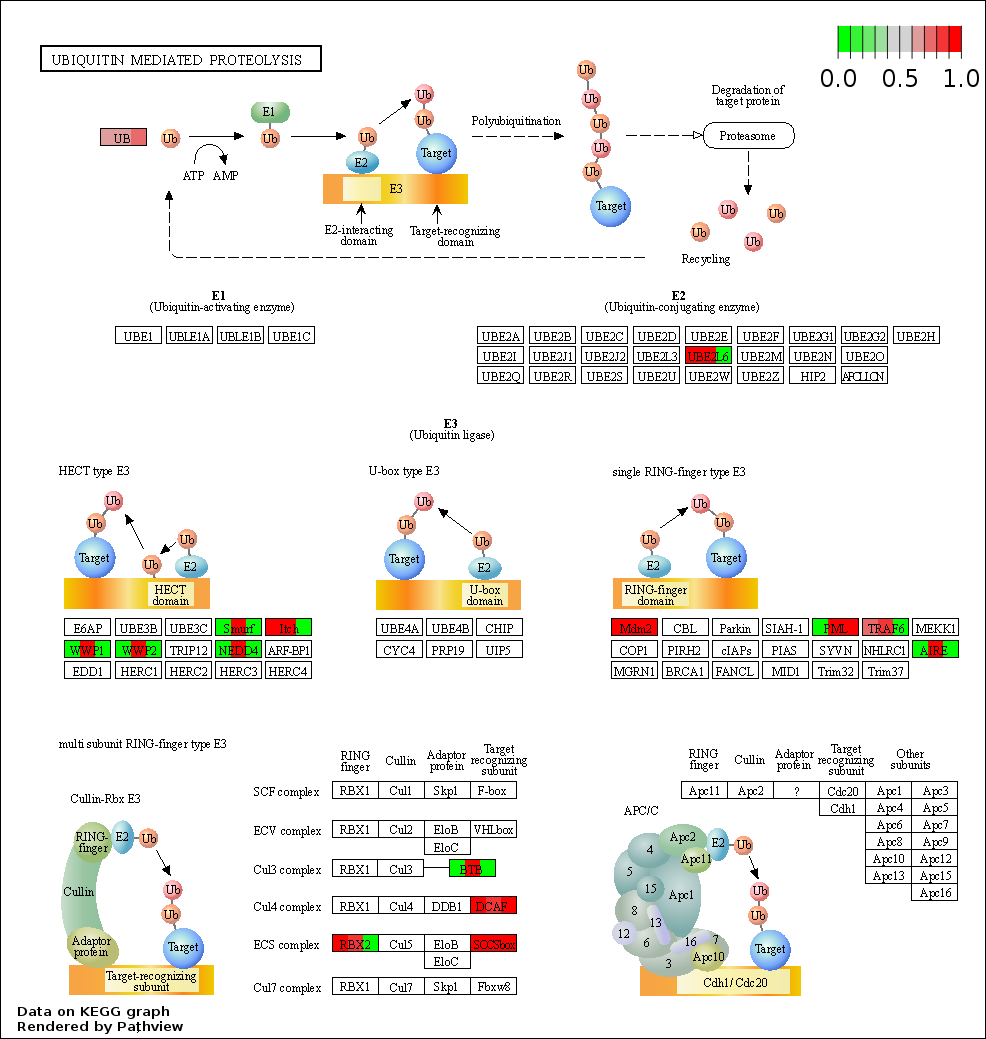
\includegraphics[height=6.3in]{figs/hsa04120.png}
    \par\end{centering}}
    \caption[Pathview Ubiquitin Mediated Proteolysis and TM Hits]{\label{Fig:Pathview_ub} The hits from the pathview analysis with TF*IDF scores providing color values with the 3 coronaviridae. Colored gene boxes from left to right are: SARS-CoV-1,SARS-CoV-2,MERS-CoV}
\end{figure}

\begin{sidewaysfigure}[!h]
    {\begin{centering}
    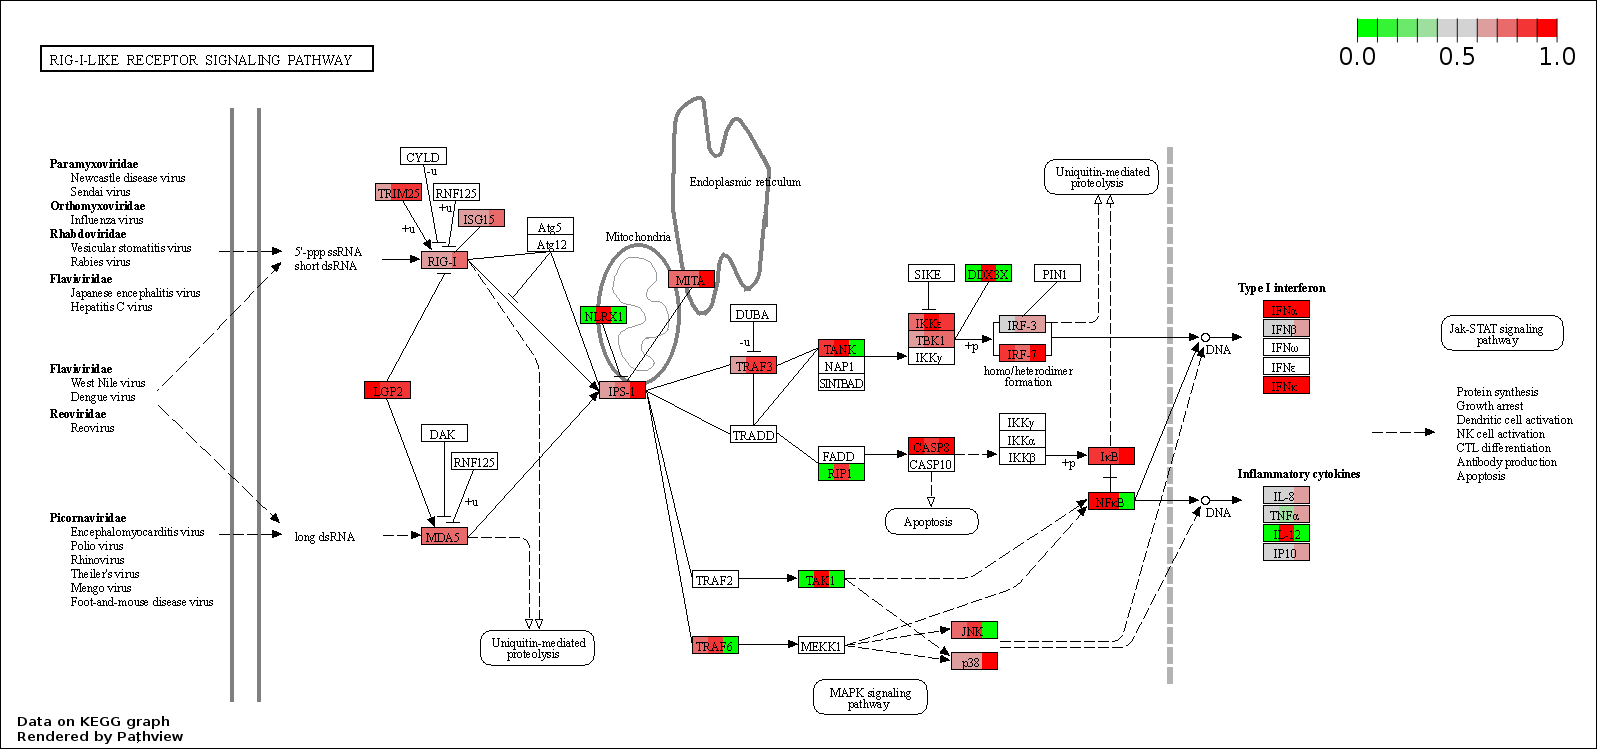
\includegraphics[height=4.2in]{figs/hsa04622.png}
    \par\end{centering}}
    \caption[Pathview RIG-I-Like Receptor Signaling Pathway and TM Hits]{\label{Fig:Pathview_rig} The hits from the pathview analysis with TF*IDF scores providing color values with the 3 coronaviridae. Colored gene boxes from left to right are: SARS-CoV-1,SARS-CoV-2,MERS-CoV}
\end{sidewaysfigure}


\end{document}